\documentclass[12pt,a4paper]{report}

% =============================================
% PACKAGES
% =============================================
\usepackage[utf8]{inputenc}
\usepackage[T1]{fontenc}
\usepackage[french]{babel}
\usepackage{csquotes}
\usepackage{tabularx}
\usepackage{geometry}
\geometry{
    top=2.5cm,
    bottom=2.5cm,
    left=2.5cm,
    right=2.5cm
}

% Graphiques et figures
\usepackage{graphicx}
\graphicspath{{figures/}}
\usepackage{float}
\usepackage{subcaption}

% Tableaux
\usepackage{booktabs}
\usepackage{array}
\usepackage{longtable}
\usepackage{multirow}
\usepackage{tabularx}

% Mathématiques
\usepackage{amsmath, amssymb, amsfonts}

% Couleurs et liens
\usepackage{xcolor}
\usepackage[hidelinks]{hyperref}

% Bibliographie
\usepackage[backend=biber, style=ieee, sorting=nyt]{biblatex}
\addbibresource{references.bib}

% Listings (code source)
\usepackage{listings}

% Définition du langage JSON pour listings
\lstdefinelanguage{json}{
  morestring=[b]",
  stringstyle=\color{orange!80!black},
  comment=[l]{//},
  commentstyle=\color{gray}\itshape,
  sensitive=false,
}

% Définition du langage JavaScript pour listings
\lstdefinelanguage{JavaScript}{
  keywords={break,case,catch,continue,debugger,default,delete,do,else,
    finally,for,function,if,in,instanceof,new,return,switch,this,throw,
    try,typeof,var,void,while,with,let,const,async,await,of,class,
    extends,import,export,from,require,module},
  keywordstyle=\color{blue}\bfseries,
  ndkeywords={true,false,null,undefined,NaN,Infinity},
  ndkeywordstyle=\color{teal},
  sensitive=true,
  comment=[l]{//},
  morecomment=[s]{/*}{*/},
  commentstyle=\color{gray}\itshape,
  stringstyle=\color{orange!80!black},
  morestring=[b]',
  morestring=[b]",
  morestring=[b]`
}

\usepackage{color}
\definecolor{gray}{rgb}{0.5,0.5,0.5}
\definecolor{orange}{rgb}{1,0.5,0}
\definecolor{teal}{rgb}{0,0.5,0.5}

\lstset{
    basicstyle=\ttfamily\footnotesize,
    breaklines=true,
    breakatwhitespace=false,
    frame=single,
    numbers=left,
    numberstyle=\tiny\color{gray},
    captionpos=b,
    keepspaces=true,
    showspaces=false,
    showstringspaces=false,
    tabsize=2,
    extendedchars=true,
    literate=
      {é}{{\'e}}1 {è}{{\`e}}1 {ê}{{\^e}}1 {ë}{{\"e}}1
      {à}{{\`a}}1 {â}{{\^a}}1 {ä}{{\"a}}1
      {î}{{\^i}}1 {ï}{{\"i}}1
      {ô}{{\^o}}1 {ö}{{\"o}}1
      {ù}{{\`u}}1 {û}{{\^u}}1 {ü}{{\"u}}1
      {ç}{{\c{c}}}1 {œ}{{\oe}}1 {æ}{{\ae}}1
      {É}{{\'E}}1 {È}{{\`E}}1 {Ê}{{\^E}}1
      {À}{{\`A}}1 {Â}{{\^A}}1
      {Î}{{\^I}}1 {Ô}{{\^O}}1 {Ù}{{\`U}}1 {Û}{{\^U}}1
      {Ç}{{\c{C}}}1
      {—}{{\textemdash}}1 {–}{{\textendash}}1
}

% TikZ
\usepackage{tikz}
\usetikzlibrary{arrows.meta, positioning, shapes.geometric, shapes.multipart, decorations.pathreplacing, calc}


% Pifont (pour \ding)
\usepackage{pifont}

% Glossaire / Acronymes
\usepackage[acronym,nonumberlist]{glossaries}
\renewcommand{\glsnamefont}[1]{\textbf{\large #1}}
\makeglossaries

% Profondeur de la table des matières
\setcounter{tocdepth}{3}
\setcounter{secnumdepth}{3}

% =============================================
% ACRONYMES
% =============================================
\newacronym{ddos}{DDoS}{Distributed Denial of Service}
\newacronym{dos}{DoS}{Denial of Service}
\newacronym{bgp}{BGP}{Border Gateway Protocol}
\newacronym{coap}{CoAP}{Constrained Application Protocol}
\newacronym{dtls}{DTLS}{Datagram Transport Layer Security}
\newacronym{dots}{DOTS}{DDoS Open Threat Signaling}
\newacronym{p2p}{P2P}{Pair-à-Pair}
\newacronym{dht}{DHT}{Distributed Hash Table}
\newacronym{spof}{SPOF}{Single Point of Failure}
\newacronym{dpi}{DPI}{Deep Packet Inspection}
\newacronym{gre}{GRE}{Generic Routing Encapsulation}
\newacronym{iot}{IoT}{Internet of Things}
\newacronym{fai}{FAI}{Fournisseur d'Accès Internet}
\newacronym{waf}{WAF}{Web Application Firewall}
\newacronym{acl}{ACL}{Access Control List}
\newacronym{cbor}{CBOR}{Concise Binary Object Representation}
\newacronym{nlri}{NLRI}{Network Layer Reachability Information}
\newacronym{as}{AS}{Autonomous System}
\newacronym{jwt}{JWT}{JSON Web Token}
\newacronym{tls}{TLS}{Transport Layer Security}
\newacronym{mtls}{mTLS}{Mutual Transport Layer Security}
\newacronym{wsm}{WSM}{Weighted Sum Model}
\newacronym{ahp}{AHP}{Analytic Hierarchy Process}
\newacronym{orm}{ORM}{Object-Relational Mapping}
\newacronym{rsa}{RSA}{Rivest-Shamir-Adleman}
\newacronym{api}{API}{Application Programming Interface}
\newacronym{rest}{REST}{Representational State Transfer}
\newacronym{uuid}{UUID}{Universally Unique Identifier}
\newacronym{rtt}{RTT}{Round-Trip Time}

% =============================================
% DEBUT DU DOCUMENT
% =============================================
\begin{document}

% ----- Pages préliminaires -----
\pagenumbering{roman}
\renewcommand{\thepage}{\textbf{\Roman{page}}}

\cleardoublepage
\thispagestyle{empty}
\chapter*{Dédicace}
\addcontentsline{toc}{chapter}{Dédicace}

\vspace*{2cm}
\begin{flushright}
\itshape

À mes très chers parents, qui ont toujours été les piliers de ma vie,\\
guidant mes pas avec une patience infinie et un amour incommensurable.\\[1.5em]

À ma mère, qui a cru en moi avant même que je ne sache ce qu'était un rêve.\\
Pour tes prières quotidiennes, ta tendresse de chaque instant\\
et ton soutien inconditionnel qui ont été mon refuge\\
et ma plus grande source de motivation tout au long de ce parcours universitaire.\\[1.5em]

À mon père, pour m'avoir inculqué le goût de l'effort,\\
la valeur du travail et la persévérance.\\
Tes sacrifices silencieux, tes précieux conseils et ta confiance absolue\\
en mes capacités m'ont donné le courage de me dépasser\\
et de mener à bien ce projet d'études.\\[1.5em]

À mes amis, mes compagnons de route,\\
qui ont partagé mes doutes, mes fous rires et mes longues nuits de révision.\\
Merci pour votre présence rassurante, vos encouragements constants\\
et pour avoir rendu ces années de formation si précieuses et inoubliables.\\[1.5em]

Enfin, à toutes les personnes qui ont cru en moi et m'ont soutenu de près ou de loin.\\
Que ce mémoire soit le fruit de votre bienveillance,\\
le reflet de vos efforts combinés aux miens,\\
et l'expression de ma profonde et éternelle gratitude.\\[2em]

\normalfont\textbf{Rania}
\end{flushright}


\cleardoublepage
\chapter*{Remerciements}
\addcontentsline{toc}{chapter}{Remerciements}

Je tiens à exprimer ma sincère gratitude à mon encadrant, M. ANANE Mohamed, et à mon promoteur, M. NAÏT-ABDESSELAM Farid, pour leur disponibilité, leurs conseils avisés et leur accompagnement tout au long de ce travail.

Je remercie les membres du jury d'avoir accepté d'évaluer ce mémoire. Leur expertise et le temps qu'ils y consacrent sont pour moi un véritable honneur.

Je tiens aussi à remercier l'École Nationale Supérieure d'Informatique pour ces cinq années de formation enrichissante, tant sur le plan académique qu'humain. Les connaissances acquises, les rencontres faites et les expériences vécues au sein de cet établissement ont profondément marqué mon parcours. Je remercie également mes camarades de promotion pour la solidarité et l'entraide qui ont marqué ces années d'études.

Enfin, j'adresse mes remerciements à ma famille et à mes amis pour leur soutien et leurs encouragements tout au long de ce parcours.



\cleardoublepage
% =======================================
% RÉSUMÉ (Français) + ABSTRACT (Anglais) 
% =======================================


% ----- Résumé français -----
\chapter*{Résumé}
\addcontentsline{toc}{chapter}{Résumé}
\markboth{Résumé}{Résumé}

Les attaques par déni de service distribué (\gls{ddos}) constituent l'une des menaces les plus critiques pour la disponibilité des services numériques modernes. Face à l'augmentation exponentielle de leur volume et de leur sophistication, les approches de mitigation centralisées montrent leurs limites~: points de défaillance uniques, coûts élevés et absence de coordination entre acteurs indépendants.

Ce mémoire a pour objectif de concevoir et d'implémenter un système distribué de mitigation collaborative des attaques \gls{ddos}, reposant sur une coalition pair-à-pair de n\oe{}uds de protection hétérogènes. Pour ce faire, le système intègre un mécanisme de confiance fondé sur le modèle PeerTrust avec crédibilité historique par session, un algorithme de sélection multicritère des pairs basé sur le Weighted Sum Model avec pondération \gls{ahp}, ainsi qu'un protocole de coordination P2P structuré en quatre phases permettant à un n\oe{}ud victime de solliciter, négocier et clore une session d'aide sans coordinateur central.

Le prototype a été développé en Node.js avec PostgreSQL et évalué sur une coalition simulée à différentes échelles. Les tests confirment la tenue en charge du système ainsi que la gestion correcte des cycles d'aide de bout en bout, depuis la détection de l'attaque jusqu'au recalcul des scores de confiance.

\medskip
\noindent\textbf{Mots-clés~:} DDoS, mitigation collaborative, pair-à-pair, confiance, PeerTrust, Weighted Sum Model, mTLS, JWT, sécurité réseau.

\newpage

% ----- Abstract anglais -----
\chapter*{Abstract}
\addcontentsline{toc}{chapter}{Abstract}
\markboth{Abstract}{Abstract}

Distributed Denial of Service (DDoS) attacks represent one of the most critical threats to the availability of modern digital services. As their volume and sophistication grow exponentially, centralized mitigation approaches show their limitations~: single points of failure, high costs, and lack of coordination between independent actors.

This thesis aims to design and implement a distributed collaborative DDoS mitigation system based on a peer-to-peer coalition of heterogeneous protection nodes. The system incorporates a trust mechanism based on the PeerTrust model with per-session historical credibility, a multi-criteria peer selection algorithm using the Weighted Sum Model with AHP weighting, and a P2P coordination protocol structured in four phases enabling a victim node to request, negotiate and close a help session without any central coordinator.

The prototype was developed in Node.js with PostgreSQL and evaluated on a simulated coalition at various scales. Tests confirm the system's ability to handle load and correctly manage end-to-end help cycles, from attack detection through trust score recalculation.

\medskip
\noindent\textbf{Keywords~:} DDoS, collaborative mitigation, peer-to-peer, trust, PeerTrust, Weighted Sum Model, mTLS, JWT, network security.

\newpage


\tableofcontents
\addcontentsline{toc}{chapter}{Table des matières}
\cleardoublepage

\printglossary[type=\acronymtype, title=Liste des acronymes]
\addcontentsline{toc}{chapter}{Liste des acronymes}
\cleardoublepage

\chapter*{Liste des abréviations}
\addcontentsline{toc}{chapter}{Liste des abréviations}

\begin{center}
\renewcommand{\arraystretch}{1.4}
\begin{longtable}{|>{\bfseries}c|l|}
\hline
\textbf{Abréviation} & \multicolumn{1}{c|}{\textbf{Signification}} \\
\hline
\endfirsthead
\hline
\textbf{Abréviation} & \multicolumn{1}{c|}{\textbf{Signification}} \\
\hline
\endhead
\hline
\endfoot
ACL   & Access Control List \\
\hline
AHP   & Analytic Hierarchy Process \\
\hline
API   & Application Programming Interface \\
\hline
AS    & Autonomous System \\
\hline
BGP   & Border Gateway Protocol \\
\hline
CBOR  & Concise Binary Object Representation \\
\hline
CoAP  & Constrained Application Protocol \\
\hline
DDoS  & Distributed Denial of Service \\
\hline
DHT   & Distributed Hash Table \\
\hline
DoS   & Denial of Service \\
\hline
DOTS  & DDoS Open Threat Signaling \\
\hline
DPI   & Deep Packet Inspection \\
\hline
DTLS  & Datagram Transport Layer Security \\
\hline
FAI   & Fournisseur d'Accès Internet \\
\hline
GRE   & Generic Routing Encapsulation \\
\hline
IoT   & Internet of Things \\
\hline
JWT   & JSON Web Token \\
\hline
mTLS  & Mutual Transport Layer Security \\
\hline
NLRI  & Network Layer Reachability Information \\
\hline
ORM   & Object-Relational Mapping \\
\hline
P2P   & Pair-à-Pair \\
\hline
REST  & Representational State Transfer \\
\hline
RSA   & Rivest-Shamir-Adleman \\
\hline
RTT   & Round-Trip Time \\
\hline
SPOF  & Single Point of Failure \\
\hline
TLS   & Transport Layer Security \\
\hline
UUID  & Universally Unique Identifier \\
\hline
WAF   & Web Application Firewall \\
\hline
WSM   & Weighted Sum Model \\
\hline
\end{longtable}
\end{center}

\cleardoublepage

\listoffigures
\addcontentsline{toc}{chapter}{Liste des figures}
\cleardoublepage

\listoftables
\addcontentsline{toc}{chapter}{Liste des tableaux}
\cleardoublepage

% ----- Corps du mémoire -----
\pagenumbering{arabic}
\setcounter{page}{1}

\chapter*{Introduction générale}
\addcontentsline{toc}{chapter}{Introduction générale}
\markboth{Introduction générale}{Introduction générale}

% -------------------------------------------------------
% Accroche et contexte général
% -------------------------------------------------------

La transformation numérique massive des organisations, l'essor du cloud et de l'Internet des objets (\gls{iot}) ont profondément renforcé la dépendance aux infrastructures réseau et aux systèmes d'information. La disponibilité continue des services numériques est devenue une exigence fondamentale, tant pour les acteurs économiques que pour les institutions et les utilisateurs. Dans cet environnement fortement interconnecté, toute interruption de service peut engendrer des conséquences opérationnelles, financières et réputationnelles significatives.

Les attaques par déni de service distribué (\gls{ddos}) constituent aujourd'hui l'une des principales menaces affectant la disponibilité des services numériques. Ces attaques consistent à générer un volume massif de trafic malveillant, distribué à partir de multiples sources, dans le but de saturer les ressources d'une cible et d'entraîner une indisponibilité partielle ou totale du service. Leur simplicité conceptuelle contraste avec leur efficacité opérationnelle, notamment lorsqu'elles exploitent des infrastructures distribuées à grande échelle et des botnets composés de milliers, voire de millions de dispositifs compromis.

Selon le rapport Cloudflare sur les menaces \gls{ddos} au premier trimestre 2025, 20,5~millions d'attaques ont été identifiées, soit une augmentation de 358\,\% par rapport à l'année précédente \cite{cloudflare2025}. Certains incidents récents ont atteint des volumes dépassant plusieurs térabits par seconde, illustrant la capacité des attaquants à mobiliser des botnets massifs et des infrastructures distribuées à grande échelle.

Les secteurs les plus ciblés incluent notamment la finance, les télécommunications, les services en ligne à forte disponibilité, ainsi que les infrastructures publiques et les plateformes de commerce électronique. Les attaques multi-vecteurs, combinant saturation volumétrique, exploitation de protocoles réseau et ciblage applicatif (couche~7), représentent désormais une part significative des incidents observés, rendant les mécanismes de défense traditionnels plus difficiles à maintenir efficaces.

Les solutions actuelles reposent majoritairement sur des architectures centralisées, telles que les \textit{scrubbing centers} ou les services de mitigation cloud. Bien que ces solutions offrent une capacité de traitement élevée, elles présentent des limites structurelles~: dépendance à un point unique de décision, latence due à la redirection du trafic, coûts élevés et absence de coordination dynamique entre acteurs indépendants.

Face à ces limites, une nouvelle approche émerge~: la \textbf{défense collaborative distribuée}. Plutôt que de traiter les attaques de manière isolée, plusieurs entités autonomes peuvent coopérer afin de partager des informations, synchroniser leurs actions et renforcer leur résilience collective. C'est dans ce cadre que s'inscrit ce projet de fin d'études \textbf{}, visant à concevoir une infrastructure de coordination inter-n\oe{}uds pour la défense collaborative contre les attaques \gls{ddos}.

% -------------------------------------------------------
% Contexte
% -------------------------------------------------------

\section*{Contexte}
\addcontentsline{toc}{section}{Contexte}

Les solutions classiques de mitigation \gls{ddos} reposent majoritairement sur des architectures centralisées, telles que des centres de nettoyage du trafic (\textit{scrubbing centers}) ou des services cloud spécialisés. Ces approches permettent d'absorber de forts volumes de trafic malveillant et d'appliquer des mécanismes de filtrage avancés. Toutefois, elles présentent plusieurs limites structurelles.

D'une part, la centralisation introduit des points de concentration critiques, susceptibles de devenir eux-mêmes des goulots d'étranglement ou des cibles d'attaque. D'autre part, les coûts associés à ces services peuvent être significatifs, ce qui limite leur accessibilité pour certaines organisations, notamment les PME et les collectivités. Enfin, la latence induite par la redirection du trafic vers des infrastructures distantes peut impacter la qualité de service.

Parallèlement, l'évolution des menaces complexifie la détection et la coordination des réponses. Les attaques modernes exploitent des botnets massifs, des vulnérabilités applicatives et des techniques d'évasion sophistiquées. Elles peuvent évoluer dynamiquement en fonction des contre-mesures mises en place. Face à ces attaques adaptatives, une simple réaction locale et isolée montre rapidement ses limites.

Dans ce cadre, l'idée d'une défense collaborative et distribuée --- reposant sur la coordination entre plusieurs n\oe{}uds de protection capables d'échanger des informations en temps réel et de mutualiser leurs ressources --- apparaît comme une piste pertinente et innovante.

% -------------------------------------------------------
% Problématique
% -------------------------------------------------------

\section*{Problématique}
\addcontentsline{toc}{section}{Problématique}

Les attaques \gls{ddos} atteignent aujourd'hui des volumes et une complexité qui dépassent les capacités de mitigation d'infrastructures isolées. Face à cette menace, les organisations utilisent principalement des solutions centralisées~: \textit{scrubbing centers} ou services cloud de mitigation.

Ces architectures présentent plusieurs limitations techniques~:
\begin{itemize}
    \item dépendance aux prestataires externes~;
    \item coûts élevés pour les PME et collectivités~;
    \item latence due à la redirection du trafic~;
    \item points uniques de défaillance (\gls{spof})~;
    \item absence de mutualisation des ressources de défense.
\end{itemize}

De plus, la défense reste individuelle. Les mécanismes actuels se limitent au partage d'informations, sans mutualisation opérationnelle des capacités de mitigation ni coordination des contre-mesures. En cas d'attaque distribuée touchant plusieurs cibles simultanément, chaque organisation réagit de son côté, ce qui réduit l'efficacité globale.

% -------------------------------------------------------
% Objectifs
% -------------------------------------------------------

\section*{Objectifs}
\addcontentsline{toc}{section}{Objectifs}

L'objectif principal de ce projet est de concevoir et d'implémenter un mécanisme de coordination inter-n\oe{}uds destiné à renforcer la défense collaborative contre les attaques \gls{ddos}.

Pour atteindre cet objectif, le travail consiste à~:
\begin{enumerate}
    \item Réaliser une étude approfondie des attaques \gls{ddos}, des mécanismes de mitigation existants et des approches collaboratives en environnement distribué.

    \item Analyser les limites des solutions centralisées actuelles et identifier les besoins en matière de coordination et de partage de ressources entre n\oe{}uds autonomes.

    \item Définir les principaux cas d'usage de coordination entre n\oe{}uds de protection, notamment l'alerte, l'entraide et la redirection de trafic.

    \item Concevoir un protocole distribué d'échange inter-n\oe{}uds précisant les règles de communication et de prise de décision.

    \item Développer un prototype permettant l'échange sécurisé de métadonnées d'attaque et la synchronisation des actions de mitigation entre plusieurs n\oe{}uds.

    \item Mettre en place un environnement de test simulant un réseau de n\oe{}uds coopérants afin d'évaluer la robustesse, la latence et la cohérence des mécanismes proposés.

    \item Réaliser une documentation technique détaillant l'architecture et le fonctionnement du système développé.
\end{enumerate}

% -------------------------------------------------------
% Organisation du rapport
% -------------------------------------------------------

\section*{Organisation du rapport}
\addcontentsline{toc}{section}{Organisation du rapport}

Le présent mémoire est structuré comme suit~:

\begin{itemize}
    \item \textbf{Chapitre~1~: Contexte et concepts fondamentaux.}
    Ce chapitre présente les fondements théoriques des attaques \gls{ddos}, la taxonomie des vecteurs d'attaque et les mécanismes de mitigation existants (\textit{scrubbing centers}, techniques de redirection, pipeline de filtrage), ainsi que les principes des architectures pair-à-pair applicables à la coordination inter-n\oe{}uds.

    \item \textbf{Chapitre~2~: État de l'art.}
    Ce chapitre propose un état de l'art des approches collaboratives et distribuées en matière de défense contre les \gls{ddos}. Cinq systèmes représentatifs sont analysés en profondeur~: \gls{dots}, DDoS Clearing House, NaWas/NBIP et DefCOM. Une synthèse comparative identifie les lacunes motivant notre contribution.

    \item \textbf{Chapitre~3~: Modélisation du système.}
    Ce chapitre décrit le modèle du système  et formalise les hypothèses retenues, les cas d'usage de coordination et les exigences fonctionnelles et non fonctionnelles.

    \item \textbf{Chapitre~4~: Conception.}
    Ce chapitre détaille la conception du protocole distribué de coordination inter-n\oe{}uds et de l'architecture d'API sécurisée pour l'échange de métadonnées d'attaque.

    \item \textbf{Chapitre~5~: Implémentation.}
    Ce chapitre présente l'implémentation du prototype  et l'environnement expérimental mis en place pour la validation.

    \item \textbf{Chapitre~6~: Résultats et évaluation.}
    Ce chapitre expose les résultats expérimentaux obtenus et leur analyse en termes de temps de réponse, de passage à l'échelle et de résilience.
\end{itemize}

Enfin, une \textbf{conclusion générale} synthétise les contributions du travail et propose des perspectives d'évolution.
% =============================================
% CHAPITRE 1 : Contexte et concepts fondamentaux
% =============================================
\chapter{Contexte et concepts fondamentaux}
\label{chap:fondamentaux}

\section{Introduction}

La sécurité des infrastructures réseau est aujourd'hui l'un des enjeux majeurs de l'informatique moderne. Parmi les menaces les plus dévastatrices, les attaques par déni de service distribué (\gls{ddos}) occupent une place prépondérante, en raison de leur capacité à paralyser des services critiques en saturant les ressources d'un ou plusieurs systèmes cibles.

Face à l'augmentation en volume et en sophistication de ces attaques, les approches de mitigation centralisées montrent rapidement leurs limites. Il devient alors indispensable d'envisager des mécanismes de défense collaborative et distribuée, où plusieurs n\oe{}uds de protection --- notamment des \textit{scrubbing centers} --- coordonnent leurs actions en temps réel pour détecter, analyser et contrer ces menaces de manière collective.

Ce chapitre a pour objectif de poser les bases conceptuelles nécessaires à la compréhension du travail présenté dans ce mémoire. Nous abordons successivement la nature et la classification des attaques \gls{ddos}, les mécanismes d'infrastructure de mitigation existants, puis les principes des systèmes distribués appliqués à la coordination inter-n\oe{}uds.

% --------------------------------------------------
\section{Les attaques par déni de service distribué (DDoS)}
\label{sec:ddos}

\subsection{Définition }

Une attaque par déni de service (\gls{dos}) désigne toute action malveillante visant à rendre un service informatique indisponible pour ses utilisateurs légitimes, en épuisant les ressources du système cible (bande passante, mémoire, CPU, connexions). Lorsque cette attaque est menée simultanément depuis un grand nombre de machines distribuées, on parle d'attaque \gls{ddos} \cite{mirkovic2004taxonomy}.

Mirkovic et Reiher définissent une attaque \gls{ddos} comme~: \og une tentative explicite d'un attaquant de nier aux utilisateurs légitimes l'utilisation d'un service réseau, en submergeant la cible ou son infrastructure intermédiaire avec du trafic illégitime \fg{} \cite{mirkovic2005dward}.


\subsection{Architecture d'une attaque DDoS}

Une attaque \gls{ddos} repose sur une architecture à plusieurs niveaux impliquant différents acteurs (voir Figure~\ref{fig:ddos_archi})~:
\begin{itemize}
    \item \textbf{L'attaquant (\textit{handler})~:} l'entité malveillante qui orchestre l'attaque depuis une machine maîtresse.
    \item \textbf{Le réseau de commande et contrôle (C\&C)~:} infrastructure permettant à l'attaquant de coordonner les agents d'attaque à distance, souvent dissimulée via des protocoles légitimes (IRC, HTTP, \gls{p2p}).
    \item \textbf{Les agents (\textit{zombies} / \textit{bots})~:} machines compromises (ordinateurs, serveurs, objets connectés \gls{iot}) qui exécutent les instructions reçues du C\&C et génèrent le trafic malveillant.
    \item \textbf{La cible (victime)~:} le système dont on cherche à épuiser les ressources --- serveur web, infrastructure DNS, routeurs de transit, etc.
\end{itemize}

\begin{figure}[htbp]
\centering
\begin{tikzpicture}[
    node distance=1.8cm and 1.6cm,
    box/.style={
        rectangle,
        draw,
        rounded corners,
        minimum width=2.2cm,
        minimum height=1cm,
        align=center,
        font=\small
    },
    arr/.style={-{Stealth[length=3mm]}, thick},
    lab/.style={font=\scriptsize}
]

\node[box, fill=red!10]    (att)  {Attaquant\\(\textit{handler})};
\node[box, fill=gray!15,   right=of att]  (cc)   {Serveur C\&C};
\node[box, fill=orange!15, right=1.8cm of cc]   (bots) {Botnet\\(zombies)};
\node[box, fill=blue!15,   right=1.8cm of bots] (vic)  {Victime\\(serveur cible)};

\draw[arr] (att) -- node[lab, above]{ordres} (cc);
\draw[arr] (cc)  -- node[lab, above]{contrôle} (bots);
\draw[arr, red!70!black] (bots) -- node[lab, above]{trafic} node[lab, below]{malveillant} (vic);

\end{tikzpicture}
\caption{Architecture générale d'une attaque DDoS.}
\label{fig:ddos_archi}
\end{figure}

Specht et Lee \cite{specht2004ddos} soulignent que la compromission de milliers voire de millions de machines forme des botnets dont la puissance agrégée dépasse largement la capacité de réponse d'un seul n\oe{}ud de défense, justifiant ainsi l'intérêt d'une défense distribuée et collaborative.

\subsection{Classification des attaques DDoS}
\label{subsec:classif_ddos}

La littérature propose plusieurs taxonomies des attaques \gls{ddos} \cite{mirkovic2004taxonomy, zargar2013survey}. Nous adoptons ici la classification en trois grandes catégories, largement répandue dans les travaux académiques et industriels. Le Tableau~\ref{tab:classif_ddos} en offre une synthèse comparative.

\subsubsection{Attaques volumétriques}

Ces attaques visent à saturer la bande passante du lien réseau de la victime ou de son \gls{fai}. Elles constituent la catégorie la plus répandue et la plus facile à générer avec un botnet. On distingue notamment~:
\begin{itemize}
    \item \textbf{UDP Flood~:} envoi massif de paquets UDP vers des ports aléatoires de la cible. L'effet principal réside dans la saturation de la bande passante par le volume brut du trafic entrant \cite{mirkovic2004taxonomy}.
    \item \textbf{ICMP Flood (\textit{Ping Flood})~:} saturation par des requêtes ICMP Echo Request en volume.
    \item \textbf{Attaques par amplification/réflexion~:} exploitation de serveurs tiers (DNS, NTP, memcached) pour amplifier le volume du trafic. L'attaquant envoie des requêtes à adresse source \textit{spoofée} (celle de la victime) vers des serveurs ouverts, qui répondent avec des paquets de taille bien supérieure. Selon Rossow \cite{rossow2014amplification}, le facteur d'amplification DNS peut atteindre 28$\times$ à 54$\times$, et celui de NTP jusqu'à 556$\times$. Les attaques via memcached ont démontré des facteurs dépassant 50\,000$\times$ \cite{chua2018memcrashed}.
\end{itemize}

\subsubsection{Attaques sur les protocoles réseau}

Ces attaques exploitent des faiblesses dans les protocoles de communication (TCP, ICMP) pour épuiser les ressources de traitement des équipements réseau intermédiaires.
\begin{itemize}
    \item \textbf{SYN Flood~:} exploitation du mécanisme de \textit{handshake} TCP en trois voies. L'attaquant envoie des paquets SYN avec adresses source \textit{spoofées}, forçant le serveur à maintenir en mémoire des connexions semi-ouvertes jusqu'à épuisement de la table d'état (\textit{backlog}). Eddy \cite{eddy2007syn} décrit en détail les vulnérabilités du protocole TCP exploitées par ce type d'attaque.
    \item \textbf{Smurf Attack~:} envoi de requêtes ICMP \textit{broadcast} avec adresse source \textit{spoofée} (celle de la victime), générant une avalanche de réponses vers la cible.
\end{itemize}

\noindent\textit{Note historique~:} Le \textit{Ping of Death}, qui consistait à envoyer des paquets ICMP de taille supérieure au maximum autorisé, a constitué une menace dans les années 1990 mais est aujourd'hui corrigé.

\subsubsection{Attaques applicatives (couche~7)}

Ces attaques ciblent la couche application du modèle OSI et sont particulièrement difficiles à distinguer du trafic légitime, car elles utilisent des requêtes HTTP, HTTPS, DNS valides du point de vue syntaxique \cite{zargar2013survey}.
\begin{itemize}
    \item \textbf{HTTP Flood~:} envoi massif de requêtes HTTP GET ou POST vers un serveur web, saturant sa capacité de traitement sans nécessiter un volume de trafic important.
    \item \textbf{Slowloris~:} maintien d'un maximum de connexions HTTP ouvertes vers le serveur cible en envoyant des en-têtes partiels à faible débit, empêchant le serveur d'accepter de nouvelles connexions légitimes.
    \item \textbf{DNS Query Flood~:} envoi massif de requêtes DNS valides pour épuiser les ressources des serveurs de noms.
\end{itemize}

\begin{table}[htbp]
\centering
\caption{Synthèse comparative des catégories d'attaques DDoS.}
\label{tab:classif_ddos}
\small

\renewcommand{\arraystretch}{1.3}

\begin{tabularx}{\textwidth}{|l|X|X|X|}
\hline
\textbf{Caractéristique} & \textbf{Volumétrique} & \textbf{Protocole} & \textbf{Applicative (L7)} \\
\hline

Couche OSI ciblée & 3--4 (Réseau~/Transport) & 3--4 (Réseau~/Transport) & 7 (Application) \\
\hline

Objectif principal & Saturer la bande passante & Épuiser les tables d'état & Épuiser les ressources applicatives \\
\hline

Volume requis & Très élevé (Gbps--Tbps) & Modéré & Faible à modéré \\
\hline

Difficulté de détection & Faible (anomalie volumétrique) & Moyenne & Élevée (trafic légitime en apparence) \\
\hline

Exemples & UDP Flood, Amplification & SYN Flood, Smurf & HTTP Flood, Slowloris \\
\hline

Mitigation typique & Filtrage, \textit{blackholing} & SYN cookies, \textit{rate limiting} & Analyse comportementale, \gls{waf} \\
\hline

\end{tabularx}
\end{table}

\subsection{Impact et données statistiques}

Les attaques \gls{ddos} engendrent des pertes économiques considérables. Selon le rapport NETSCOUT Threat Intelligence Report 2023, plus de 7,9~millions d'attaques \gls{ddos} ont été enregistrées sur la seule première moitié de l'année 2023, soit une moyenne de plus de 44\,000 attaques par jour \cite{netscout2023}. Zargar et al. \cite{zargar2013survey} estiment que le coût moyen d'une attaque \gls{ddos} pour une entreprise peut dépasser 50\,000~dollars par heure d'interruption de service, incluant les pertes commerciales directes, les coûts de mitigation et les dommages réputationnels.

% --------------------------------------------------
\section{Infrastructure de mitigation DDoS}
\label{sec:mitigation}

La mitigation des attaques \gls{ddos} repose sur un ensemble d'infrastructures et de techniques déployées à différents niveaux du réseau. Cette section présente les principales solutions existantes, leurs mécanismes de fonctionnement et leurs limites respectives.

\subsection{Les \textit{scrubbing centers}~: définition et rôle}

Un \textit{scrubbing center} (ou centre de nettoyage du trafic) est une infrastructure spécialisée dont la mission est d'analyser le trafic réseau entrant, de filtrer les paquets malveillants, puis de renvoyer uniquement le trafic légitime vers la destination finale. Ce mécanisme est souvent désigné sous le terme de \og \textit{clean pipe} \fg{} \cite{mahajan2002controlling}.

Le processus de mitigation via \textit{scrubbing center} se déroule en plusieurs étapes distinctes (voir Figure~\ref{fig:scrubbing})~:
\begin{enumerate}
    \item \textbf{Détection~:} une anomalie dans le trafic déclenche une alerte (analyse NetFlow/sFlow, seuils de bande passante, corrélation multi-sources).
    \item \textbf{Redirection~:} le trafic destiné à la victime est redirigé vers le \textit{scrubbing center} via des mécanismes de routage (\gls{bgp}, DNS).
    \item \textbf{Analyse et filtrage~:} le centre analyse le trafic en appliquant un pipeline de traitement multi-couches (empreintes, comportement, limitation de débit).
    \item \textbf{Réinjection~:} le trafic nettoyé est retransmis à la victime via un tunnel \gls{gre} ou MPLS pour éviter les boucles de routage.
\end{enumerate}
\begin{figure}[htbp]
\centering
\begin{tikzpicture}[
    node distance=0.8cm,
    stp/.style={
        rectangle, draw, rounded corners,
        minimum width=2.4cm,
        minimum height=1.1cm,
        align=center, font=\small
    },
    arr/.style={-{Stealth[length=3mm]}, thick}
]

\node[stp, fill=blue!10]   (det) {1. Détection\\Anomalie};
\node[stp, fill=orange!15, right=of det] (red) {2. Redirection\\BGP / DNS};
\node[stp, fill=red!10,    right=of red] (fil) {3. Filtrage\\DPI, Rate limit};
\node[stp, fill=green!15,  right=of fil] (rei) {4. Réinjection\\GRE / MPLS};

\draw[arr] (det) -- (red);
\draw[arr] (red) -- (fil);
\draw[arr] (fil) -- (rei);

\draw[arr, red!70, dashed] ($(det.west)+(-1.5,0)$) -- (det.west)
    node[midway, above, font=\scriptsize] {Trafic}
    node[midway, below, font=\scriptsize] {entrant};

\draw[arr, green!60!black, dashed] (rei.east) -- ++(1.5,0)
    node[midway, above, font=\scriptsize] {Trafic}
    node[midway, below, font=\scriptsize] {légitime};

\end{tikzpicture}
\caption{Processus de mitigation via un \textit{scrubbing center}.}
\label{fig:scrubbing}
\end{figure}

Parmi les principaux fournisseurs de \textit{scrubbing centers}, on trouve des acteurs comme Arbor Networks (Sightline/TMS), Akamai (Prolexic), Radware (DefensePro) et A10 Networks (Thunder TPS). Ces solutions offrent des capacités de traitement allant de quelques dizaines de Gbps à plusieurs Tbps selon l'infrastructure déployée.

% ----- NOUVELLE SOUS-SECTION -----
\subsection{Les réseaux de diffusion de contenu (CDN) comme bouclier anti-DDoS}

Les \textbf{CDN} (\textit{Content Delivery Networks}) tels que Cloudflare, Akamai et AWS CloudFront constituent une autre ligne de défense majeure contre les attaques \gls{ddos}. Leur principe repose sur la \textbf{distribution géographique} du contenu et du traitement du trafic à travers un réseau mondial de points de présence (PoP).

Le mécanisme de protection d'un CDN fonctionne comme suit~:
\begin{enumerate}
    \item \textbf{Interception par DNS~:} les enregistrements DNS de la victime sont modifiés pour pointer vers les serveurs du CDN. Tout le trafic entrant transite donc par le réseau du CDN avant d'atteindre le serveur d'origine.
    \item \textbf{Absorption volumétrique~:} grâce à la technique \textbf{Anycast}, le même préfixe IP est annoncé depuis des centaines de PoP répartis mondialement. Le trafic est automatiquement dirigé vers le PoP le plus proche géographiquement, ce qui \textbf{distribue naturellement} la charge d'une attaque volumétrique sur l'ensemble du réseau.
    \item \textbf{Filtrage en bordure~:} chaque PoP applique des règles de filtrage (limitation de débit, \gls{waf}, challenges JavaScript/CAPTCHA) pour bloquer le trafic malveillant avant qu'il n'atteigne le serveur d'origine.
    \item \textbf{Transmission du trafic légitime~:} seul le trafic validé est transmis au serveur d'origine via un canal sécurisé (HTTPS).
\end{enumerate}

\begin{figure}[htbp]
\centering
\begin{tikzpicture}[
    node distance=1.5cm and 2cm,
    box/.style={
        rectangle, draw, rounded corners,
        minimum width=2cm,
        minimum height=0.8cm,
        align=center, font=\small
    },
    arr/.style={-{Stealth[length=3mm]}, thick}
]
    \node[box, fill=red!15]    (att) {Attaquants};
    \node[box, fill=gray!10,   right=of att] (dns) {DNS\\Anycast};
    \node[box, fill=orange!15, right=of dns, yshift=0.8cm]  (pop1) {PoP Europe};
    \node[box, fill=orange!15, right=of dns]                (pop2) {PoP Asie};
    \node[box, fill=orange!15, right=of dns, yshift=-0.8cm] (pop3) {PoP USA};
    \node[box, fill=blue!15,   right=2.5cm of pop2] (origin) {Serveur\\d'origine};

    \draw[arr, red] (att) -- (dns);
    \draw[arr] (dns) -- (pop1);
    \draw[arr] (dns) -- (pop2);
    \draw[arr] (dns) -- (pop3);
    \draw[arr, green!60!black] (pop1) -- (origin);
    \draw[arr, green!60!black] (pop2) -- (origin);
    \draw[arr, green!60!black] (pop3) -- (origin);

    \node[font=\scriptsize\itshape, text=red!60, below=0.3cm of dns] {Trafic distribué};
    \node[font=\scriptsize\itshape, text=green!50!black, above=0.1cm of origin] {Trafic propre};
\end{tikzpicture}
\caption{Principe de protection anti-DDoS par un CDN avec Anycast.}
\label{fig:cdn_protection}
\end{figure}

Cependant, les CDN présentent des limites~:
\begin{itemize}
    \item \textbf{Protection limitée à la couche applicative (HTTP/HTTPS)~:} les CDN protègent principalement les services web. Les attaques ciblant d'autres protocoles (DNS autoritaire, VoIP, jeux en ligne, VPN) ne bénéficient pas de cette protection.
    \item \textbf{Dépendance à un fournisseur tiers~:} l'ensemble du trafic transite par l'infrastructure du CDN, créant une dépendance forte et un risque de confidentialité.
    \item \textbf{Coûts variables~:} la tarification au volume peut devenir prohibitive lors d'attaques massives prolongées.
\end{itemize}

% ----- NOUVELLE SOUS-SECTION -----
\subsection{Les pare-feu et systèmes de prévention d'intrusion (IPS)}

Les \textbf{pare-feu} (\textit{firewalls}) et les \textbf{systèmes de prévention d'intrusion} (\textit{Intrusion Prevention Systems} --- IPS) constituent la première ligne de défense déployée en périphérie du réseau de l'organisation.

\subsubsection{Pare-feu traditionnels et nouvelle génération (NGFW)}

Les pare-feu filtrent le trafic réseau en fonction de règles prédéfinies basées sur les adresses IP, les ports et les protocoles. Les \textbf{pare-feu de nouvelle génération} (NGFW --- \textit{Next-Generation Firewall}) ajoutent des capacités d'inspection applicative~:
\begin{itemize}
    \item \textbf{Inspection à états (\textit{stateful inspection})~:} suivi des connexions TCP pour détecter les anomalies (SYN Flood, connexions incomplètes).
    \item \textbf{Inspection applicative (couche~7)~:} analyse du contenu des paquets pour identifier les requêtes malveillantes (injections SQL, requêtes HTTP anormales).
    \item \textbf{Limitation de débit (\textit{rate limiting})~:} restriction du nombre de connexions par source IP et par unité de temps.
\end{itemize}

\subsubsection{Systèmes de prévention d'intrusion (IPS)}

Les IPS analysent le trafic en temps réel pour détecter et bloquer les comportements malveillants en se basant sur~:
\begin{itemize}
    \item \textbf{Signatures~:} correspondance avec une base de signatures d'attaques connues (similaire aux antivirus).
    \item \textbf{Anomalies~:} détection de déviations par rapport à un profil de trafic normal (\textit{baseline}).
    \item \textbf{Heuristiques~:} analyse comportementale combinant plusieurs indicateurs pour détecter des attaques inconnues (\textit{zero-day}).
\end{itemize}

\textbf{Limites face aux attaques DDoS~:} les pare-feu et IPS sont dimensionnés pour le volume de trafic \textit{normal} de l'organisation. Lors d'une attaque volumétrique, le pare-feu lui-même devient un goulot d'étranglement~: sa capacité de traitement (mesurée en paquets par seconde --- pps) est rapidement dépassée, ce qui peut provoquer l'effondrement de l'ensemble du périmètre de sécurité. De plus, les pare-feu à états consomment de la mémoire pour chaque connexion suivie, les rendant particulièrement vulnérables aux attaques d'épuisement de tables d'état (SYN Flood, TCP connection exhaustion).

% ----- NOUVELLE SOUS-SECTION -----
\subsection{Le \textit{blackholing} et le RTBH (\textit{Remote Triggered Black Hole})}

Le \textbf{\textit{blackholing}} est une technique de dernier recours qui consiste à rediriger l'intégralité du trafic destiné à une adresse IP attaquée vers une route nulle (\texttt{null0} / \textit{bit bucket}), supprimant ainsi tout le trafic --- légitime et malveillant --- vers cette destination.

Le mécanisme \textbf{RTBH} (\textit{Remote Triggered Black Hole}, RFC~5635 \cite{kumari2009rtbh}) permet d'automatiser ce processus via \gls{bgp}~:
\begin{enumerate}
    \item Le réseau victime annonce le préfixe attaqué avec une \textbf{communauté BGP spéciale} (ex.~: \texttt{AS:666}) à ses fournisseurs de transit.
    \item Les routeurs des fournisseurs de transit, configurés pour reconnaître cette communauté, redirigent le trafic vers \texttt{null0}.
    \item Le trafic d'attaque est ainsi éliminé \textit{en amont}, avant qu'il ne sature les liens du réseau victime.
\end{enumerate}

\begin{figure}[htbp]
\centering
\begin{tikzpicture}[
    node distance=2cm and 2.8cm,
    box/.style={
        rectangle, draw, rounded corners,
        minimum width=2.5cm, minimum height=1cm,
        align=center, font=\small
    },
    arr/.style={-{Stealth[length=3mm]}, thick},
    lab/.style={font=\scriptsize}
]

% --- Nœuds ---
\node[box, fill=red!10]   (att)     {Attaquants};
\node[box, fill=gray!10,  right=of att]     (transit) {FAI Transit};
\node[box, fill=blue!10,  right=of transit] (victim)  {Victime};
\node[box, fill=black!10, below=2.5cm of transit] (null)
    {\texttt{null0}\\(Black hole)};

% 1. Trafic d'attaque → FAI Transit
\draw[arr, red] (att) -- 
    node[lab, above] {trafic d'attaque} (transit);

% 2. Acheminement normal sans RTBH (chemin supérieur)
\draw[arr, red, dashed] (transit.15) -- 
    node[lab, above] {sans RTBH} (victim.165);

% 3. Avec RTBH : drop vers null0
\draw[arr, orange] (transit.south) -- 
    node[lab, left, align=center] {avec RTBH\\drop} (null.north);

% 4. Signalisation BGP : victime → transit (chemin inférieur)
\draw[arr, blue, dashed] (victim.-165) -- 
    node[lab, below, align=center, inner sep=2pt] 
    {Annonce BGP\\communauté RTBH (\texttt{AS:666})} 
    (transit.-15);

\end{tikzpicture}
\caption{Mécanisme de RTBH via BGP~: la victime annonce un préfixe 
avec une communauté RTBH, et le FAI redirige le trafic correspondant 
vers \texttt{null0}.}
\label{fig:rtbh}
\end{figure}

\textbf{Avantage~:} le \textit{blackholing} est extrêmement efficace pour protéger l'infrastructure réseau (les liens ne sont plus saturés).

\textbf{Inconvénient majeur~:} il constitue une \textbf{victoire de l'attaquant}. En supprimant tout le trafic vers la cible --- y compris le trafic légitime ---, le \textit{blackholing} produit exactement le résultat recherché par l'attaque~: le déni de service. C'est pourquoi cette technique n'est utilisée qu'en dernier recours, lorsque le sacrifice d'un service est préférable à l'effondrement de l'infrastructure complète.

% ----- NOUVELLE SOUS-SECTION -----
\subsection{Les services de mitigation cloud (\textit{Cloud-based DDoS Protection})}

Les \textbf{services de mitigation cloud} sont proposés par des fournisseurs spécialisés (Cloudflare, AWS Shield, Azure DDoS Protection, Google Cloud Armor) qui disposent d'une infrastructure mondiale massive pour absorber les attaques \gls{ddos}.

Le fonctionnement repose sur le même principe que les \textit{scrubbing centers}, mais avec deux différences majeures~:
\begin{itemize}
    \item \textbf{Capacité élastique~:} les fournisseurs cloud disposent de capacités de traitement pouvant dépasser 100~Tbps en cumulé sur l'ensemble de leurs PoP, ce qui leur permet d'absorber les attaques les plus volumétriques.
    \item \textbf{Modèle \textit{as-a-Service}~:} la mitigation est proposée sous forme d'abonnement, évitant à l'organisation d'investir dans une infrastructure physique dédiée.
\end{itemize}

Le Tableau~\ref{tab:services_cloud} compare les principaux services de mitigation cloud disponibles sur le marché.

\begin{table}[htbp]
\centering
\caption{Comparaison des principaux services de mitigation cloud.}
\label{tab:services_cloud}
\small
\renewcommand{\arraystretch}{1.4}
\begin{tabularx}{\textwidth}{|l|X|X|X|}
\hline
\textbf{Service} & \textbf{Capacité} & \textbf{Couches protégées} & \textbf{Activation} \\
\hline
Cloudflare       & 348~Tbps (réseau global) & L3/L4 + L7 (WAF intégré) & Always-on (automatique) \\
\hline
AWS Shield Advanced & Élastique (infra AWS) & L3/L4 + L7 (avec WAF) & Always-on + sur demande \\
\hline
Azure DDoS Protection & Élastique (infra Azure) & L3/L4 & Always-on \\
\hline
Google Cloud Armor & Élastique (infra Google) & L7 (HTTP/HTTPS) & Always-on \\
\hline
Akamai Prolexic  & 20+ Tbps (scrubbing dédié) & L3/L4 + L7 & On-demand (BGP redirect) \\
\hline
\end{tabularx}
\end{table}

\textbf{Limites des services cloud~:}
\begin{itemize}
    \item \textbf{Dépendance au fournisseur~:} l'organisation confie l'intégralité de son trafic à un tiers, ce qui soulève des questions de confidentialité, de souveraineté des données et de \textit{vendor lock-in}.
    \item \textbf{Coûts récurrents~:} les abonnements premium (ex.~: AWS Shield Advanced à 3\,000~\$/mois + coûts de transfert de données) peuvent être prohibitifs pour les petites structures.
    \item \textbf{Latence additionnelle~:} le reroutage du trafic via le réseau du fournisseur ajoute une latence (typiquement 5 à 30~ms selon la distance au PoP le plus proche).
    \item \textbf{Absence de coordination inter-fournisseurs~:} chaque service opère de manière isolée. Il n'existe pas de mécanisme standardisé pour que Cloudflare, AWS et Akamai coordonnent leurs actions face à une attaque ciblant simultanément plusieurs de leurs clients.
\end{itemize}

% ----- NOUVELLE SOUS-SECTION -----
\subsection{Techniques de redirection du trafic}

La redirection du trafic vers une infrastructure de mitigation (qu'il s'agisse d'un \textit{scrubbing center}, d'un CDN ou d'un service cloud) est une opération critique. Plusieurs techniques sont utilisées en pratique~:
\begin{itemize}
    \item \textbf{\gls{bgp} Blackholing et BGP Flowspec~:} Le protocole \gls{bgp} (RFC~4271 \cite{rekhter2006bgp}) permet d'annoncer des préfixes IP pour rediriger le trafic. Le BGP Flowspec (RFC~5575 \cite{marques2009flowspec}) étend cette capacité en distribuant des règles de filtrage fin (correspondance sur les champs source/destination IP, port, protocole, taille de paquet, fragment) sous forme de \gls{nlri} multi-champs, permettant aux routeurs de bordure d'appliquer des actions (\texttt{discard}, \texttt{rate-limit}, \texttt{redirect} vers VRF) sans intervention manuelle.
    \item \textbf{DNS Redirection~:} Modification des enregistrements DNS de la victime pour pointer vers l'infrastructure de mitigation. Technique utilisée par les CDN (Cloudflare, Akamai) et les services cloud.
    \item \textbf{Anycast~:} Déploiement du même préfixe IP sur plusieurs n\oe{}uds distribués géographiquement, permettant une absorption distribuée naturelle. Le trafic est dirigé vers le n\oe{}ud le plus proche selon la topologie \gls{bgp}.
    \item \textbf{Tunnel GRE/MPLS~:} Encapsulation du trafic nettoyé pour le renvoyer à la victime via un chemin distinct (\textit{clean-return path}), évitant les boucles de routage.
\end{itemize}

% ----- NOUVELLE SOUS-SECTION -----
\subsection{Synthèse et comparaison des infrastructures de mitigation}

Le Tableau~\ref{tab:comparaison_infra} compare les différentes infrastructures de mitigation présentées dans cette section selon plusieurs critères clés.

\begin{table}[htbp]
\centering
\caption{Comparaison des infrastructures de mitigation DDoS.}
\label{tab:comparaison_infra}
\small
\renewcommand{\arraystretch}{1.4}
\begin{tabularx}{\textwidth}{|l|X|X|X|X|}
\hline
\textbf{Solution} & \textbf{Couches} & \textbf{Capacité} & \textbf{Avantage principal} & \textbf{Limite principale} \\
\hline
Scrubbing center & L3/L4/L7 & Élevée (Tbps) & Filtrage fin multi-couches & Coût, latence de redirection \\
\hline
CDN (Anycast)    & L7 (HTTP) & Très élevée & Distribution géographique & Limité au trafic web \\
\hline
Pare-feu / IPS   & L3/L4/L7 & Limitée (Gbps) & Proximité, contrôle local & Goulot d'étranglement \\
\hline
RTBH Blackholing & L3 & Illimitée & Protège l'infrastructure & Supprime le trafic légitime \\
\hline
Service cloud    & L3/L4/L7 & Élastique & Capacité massive, as-a-Service & Dépendance, coût, confidentialité \\
\hline
\end{tabularx}
\end{table}

% ----- SOUS-SECTION EXISTANTE ENRICHIE -----
\subsection{Limites des approches centralisées}

Bien que les solutions présentées ci-dessus offrent chacune des capacités de mitigation significatives, elles partagent un trait commun~: elles opèrent de manière \textbf{centralisée et isolée}. Chaque organisation déploie ses propres défenses ou souscrit à un service individuel, sans mécanisme de coordination avec les autres entités potentiellement touchées par la même attaque.

Cette approche présente plusieurs limites fondamentales \cite{douligeris2004ddos}~:
\begin{itemize}
    \item \textbf{Point de défaillance unique (\gls{spof})~:} que ce soit le \textit{scrubbing center}, le contrôleur SDN ou le fournisseur cloud, toute architecture centralisée introduit un point critique dont la défaillance compromet l'ensemble de la protection.
    \item \textbf{Latence de redirection~:} le reroutage du trafic vers une infrastructure distante introduit une latence additionnelle (10 à 50~ms) qui dégrade la qualité de service pour les applications sensibles (VoIP, jeux en ligne, trading haute fréquence).
    \item \textbf{Capacité finie~:} même les plus grandes infrastructures ont une capacité maximale. Face à une attaque dépassant cette capacité, la solution centralisée est elle-même submergée.
    \item \textbf{Visibilité locale~:} chaque solution n'observe que le trafic qui lui est redirigé. Elle ne peut pas corréler ses observations avec celles d'autres infrastructures pour détecter des attaques coordonnées ciblant simultanément plusieurs victimes.
    \item \textbf{Absence de mutualisation~:} les ressources de mitigation de différentes organisations ne sont pas partagées. Un \textit{scrubbing center} sous-utilisé ne peut pas venir en aide à un voisin surchargé.
    \item \textbf{Coûts prohibitifs~:} le dimensionnement d'une infrastructure capable d'absorber les attaques les plus volumétriques (multi-Tbps) représente un investissement considérable, inaccessible aux PME et aux petites collectivités.
\end{itemize}

Ces limitations convergent vers un constat~: \textbf{la défense isolée ne suffit plus}. La réponse aux attaques \gls{ddos} modernes nécessite une approche \textbf{collaborative et distribuée}, où plusieurs entités autonomes coordonnent leurs actions en temps réel pour mutualiser leurs capacités de détection, d'analyse et de filtrage. C'est cette approche que nous développons dans ce mémoire.
% --------------------------------------------------
\section{Architecture pair-à-pair pour la coordination inter-n\oe{}uds}
\label{sec:p2p}

\subsection{Définition et pertinence du modèle pair-à-pair}

Une architecture \gls{p2p} est un modèle de système distribué dans lequel les n\oe{}uds (ou pairs) sont logiquement équivalents et peuvent assumer simultanément les rôles de client et de serveur. Contrairement aux architectures centralisées traditionnelles, aucun n\oe{}ud ne joue le rôle d'autorité de contrôle unique \cite{tanenbaum2017distributed}. Chaque pair peut ainsi fournir des services aux autres tout en consommant leurs ressources.

Dans le contexte de la mitigation des attaques \gls{ddos}, ce modèle apparaît particulièrement pertinent pour répondre aux limites des architectures centralisées identifiées précédemment (cf. section~1.3.8). En structurant différents mécanismes de défense — tels que les \textit{scrubbing centers}, les pare-feu ou les systèmes de détection — au sein d'un réseau logique superposé (\textit{overlay network}), l'architecture \gls{p2p} permet de répartir les capacités de détection et de filtrage entre plusieurs entités autonomes.

Une telle organisation repose sur trois principes fondamentaux :

\begin{itemize}
    \item \textbf{Décentralisation :} l'absence de point de contrôle central élimine les points de défaillance uniques (\gls{spof}) et renforce la résilience globale de l'infrastructure de défense.
    
    \item \textbf{Autonomie et coopération :} chaque n\oe{}ud conserve la maîtrise de ses ressources locales tout en participant à un mécanisme de défense collectif, permettant de mutualiser les capacités de détection et de mitigation.
    
    \item \textbf{Symétrie des rôles :} un même pair peut signaler une attaque lorsqu'il est victime et contribuer simultanément à la mitigation en appliquant des règles de filtrage ou en relayant des informations vers d'autres pairs.
\end{itemize}

Cette approche ouvre la voie à des mécanismes de défense collaborative où plusieurs organisations peuvent coordonner leurs actions afin de limiter l'impact d'attaques distribuées à grande échelle.

\subsection{Topologies et protocoles P2P applicables à la mitigation}

Les systèmes \gls{p2p} peuvent adopter différentes formes d'organisation, dont l'efficacité varie selon les objectifs et les contraintes du système distribué \cite{tanenbaum2017distributed}. Dans le cadre d'une infrastructure de défense collaborative, plusieurs modèles sont particulièrement pertinents.

\begin{itemize}

\item \textbf{P2P non structuré :}  
Dans ce modèle, les n\oe{}uds établissent des connexions de manière ad hoc sans structure globale prédéfinie. La recherche d'information ou la diffusion d'alertes s'effectue généralement par inondation (\textit{flooding}). Bien que cette approche soit très robuste face à la disparition de pairs, elle entraîne une surcharge réseau importante et devient difficilement scalable dans des environnements comportant un grand nombre de participants.

\item \textbf{P2P structuré (\gls{dht}) :}  
Les architectures structurées reposent sur une topologie logique déterministe, souvent implémentée à l'aide d'une table de hachage distribuée (\gls{dht}). Des systèmes tels que Chord \cite{stoica2001chord} permettent de localiser une information en $O(\log N)$ sauts. Dans le contexte de la défense \gls{ddos}, une \gls{dht} peut être utilisée pour maintenir une base de données distribuée contenant des indicateurs de compromission, des signatures d'attaques ou des listes d'adresses IP malveillantes partagées entre participants.

\item \textbf{P2P hybride :}  
Les architectures hybrides introduisent la notion de \textit{super-pairs}. Certains n\oe{}uds disposant de capacités importantes (par exemple des \textit{scrubbing centers} ou des n\oe{}uds c\oe{}ur de réseau d'un \gls{fai}) jouent un rôle de coordination ou d'agrégation, tandis que des n\oe{}uds périphériques participent à l'échange d'informations avec des capacités plus limitées. Ce modèle permet d'améliorer l'efficacité du routage des messages tout en conservant un degré de décentralisation.

\item \textbf{Protocoles épidémiques (\textit{gossip}) :}  
Les protocoles \textit{gossip} reposent sur une diffusion probabiliste de l'information. Chaque n\oe{}ud transmet périodiquement son état ou une alerte à un sous-ensemble aléatoire de ses voisins. Cette approche offre une forte tolérance aux pannes et permet une propagation rapide des informations, généralement en $O(\log N)$ cycles de communication. Dans le cadre d'une défense collaborative, les mécanismes \textit{gossip} sont particulièrement adaptés pour diffuser rapidement des alertes d'attaque ou des règles de mitigation sans saturer le réseau de communication.

\end{itemize}

\subsection{Défis du P2P appliqué à la sécurité réseau}

Malgré ses avantages, l'application d'un modèle distribué à la coordination d'infrastructures de défense appartenant à des entités indépendantes soulève plusieurs défis majeurs.

\begin{itemize}

\item \textbf{Gestion de la confiance :}  
Dans un système décentralisé, l'absence d'autorité centrale complique la validation de l'identité et de la fiabilité des pairs. Un n\oe{}ud compromis pourrait diffuser de fausses alertes afin de provoquer un blocage injustifié du trafic légitime (\textit{blackholing} offensif) ou créer de multiples identités afin d'influencer les décisions collectives (attaque \textit{Sybil}). La mise en place de mécanismes d'authentification forte ou de systèmes de réputation devient alors indispensable.

\item \textbf{Latence de convergence :}  
Les attaques \gls{ddos} volumétriques peuvent saturer les ressources d'une cible en quelques secondes. La propagation des alertes et la synchronisation des mécanismes de filtrage entre pairs doivent donc être extrêmement rapides afin que la mitigation distribuée puisse être effective avant l'effondrement du service attaqué.

\item \textbf{Problème du passager clandestin (\textit{free-rider}) :}  
La mitigation d'attaques distribuées nécessite des ressources importantes en bande passante et en capacité de traitement. Dans un système coopératif ouvert, certains participants pourraient bénéficier de la protection collective sans contribuer réellement à l'effort de mitigation. Des mécanismes d'incitation à la coopération, tels que des quotas de contribution ou des systèmes de réputation, peuvent être nécessaires pour limiter ce comportement.

\item \textbf{Passage à l'échelle sous contrainte réseau :}  
Lors d'une attaque de grande ampleur, le plan de données du réseau peut subir une congestion importante. Le réseau de coordination \gls{p2p} — qui constitue le plan de contrôle du système — doit donc rester opérationnel même en présence de pertes de paquets élevées ou de fortes variations de latence.

\end{itemize}

Ces défis expliquent pourquoi la mise en œuvre de mécanismes de défense véritablement distribués reste complexe dans la pratique. Les approches existantes tentant d'exploiter ces principes seront analysées dans le chapitre suivant à travers l'étude de plusieurs systèmes représentatifs de la littérature.
% --------------------------------------------------
\section{Conclusion}

Ce chapitre a posé les fondements nécessaires à la compréhension du travail présenté dans ce mémoire. Nous avons défini les attaques \gls{ddos} et leurs catégories (volumétriques, protocolaires, applicatives), décrit l'infrastructure de mitigation actuelle (\textit{scrubbing centers}) et ses limites centralisées, puis introduit l'architecture \gls{p2p} comme solution potentielle de coordination entre n\oe{}uds de défense.

Le chapitre suivant analyse les principales approches existantes en matière de défense collaborative contre les attaques DDoS.
% =============================================
% CHAPITRE 2 : Étude bibliographique
% =============================================
\chapter{Étude bibliographique}
\label{chap:etat_art}

\section{Introduction}

La défense collaborative contre les attaques \gls{ddos} a donné lieu à une littérature académique riche ainsi qu'à plusieurs déploiements institutionnels et industriels. Ce chapitre analyse quatre contributions majeures, sélectionnées pour leur représentativité des différentes approches existantes~:
\begin{itemize}
    \item un standard de signalisation inter-domaines (\gls{dots}),
    \item une coalition nationale de partage de métadonnées (DDoS Clearing House),
    \item une mutualisation opérationnelle de \textit{scrubbing centers} (NaWas/NBIP),
    \item un overlay coopératif distribué (DefCOM).
\end{itemize}

Pour chaque travail, nous décrivons le contexte de sa conception, son architecture technique détaillée, ses mécanismes protocolaires et ses limites identifiées. Une synthèse comparative clôt le chapitre et identifie les lacunes que notre contribution vise à combler.

% --------------------------------------------------
\section{DOTS --- DDoS Open Threat Signaling}
\label{sec:dots}

\subsection{Contexte et motivation}

L'IETF a initié le groupe de travail \gls{dots} (\textit{DDoS Open Threat Signaling}) pour définir un protocole standardisé permettant à une entité attaquée de notifier automatiquement un prestataire de mitigation. Les exigences sont formalisées dans la RFC~8612 \cite{mortensen2019dots} et le canal de signalisation dans la RFC~8782 \cite{reddy2020dots}.

\subsection{Architecture et fonctionnement}

\gls{dots} repose sur une architecture client--serveur asymétrique comprenant un \textbf{DOTS client} (l'entité sous attaque) et un \textbf{DOTS server} (le prestataire de mitigation).

Le protocole s'appuie sur une pile technologique légère adaptée aux environnements contraints et congestionnés, divisée en deux canaux distincts (voir Figure~\ref{fig:dots_archi})~:


\begin{figure}[htbp]
\centering
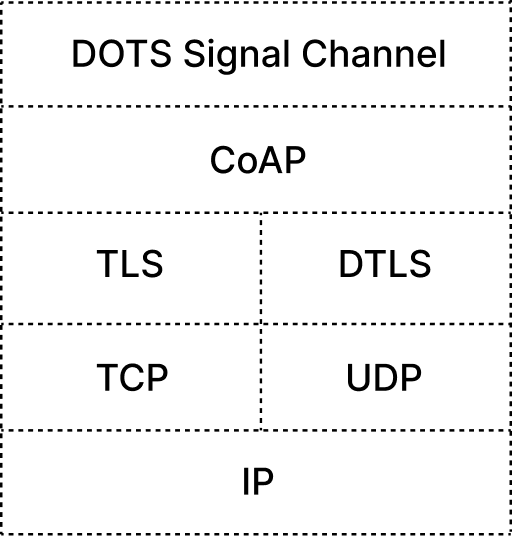
\includegraphics [height=0.45\textwidth]{do.png}

\caption{Architecture de référence du protocole \gls{dots} : séparation entre le canal de signalisation (CoAP/DTLS/UDP) et le canal de données (RESTCONF/HTTPS/TCP).}

\label{fig:dots_archi}
\end{figure}


\subsubsection{Canal de signalisation (\textit{Signal Channel})}

Ce canal utilise le protocole \gls{coap} (\textit{Constrained Application Protocol}, RFC~7252) sécurisé par \gls{dtls}~1.2 (RFC~6347) sur UDP. Ce choix est stratégique~: contrairement à TCP, UDP évite les délais de retransmission et le blocage de tête de ligne (\textit{Head-of-Line blocking}) fréquents lors d'une saturation de lien.

Concrètement, le client émet une requête CoAP \texttt{PUT} sur l'URI~:
\begin{center}
    \texttt{/dots/signal/\{cuid\}/\{mid\}}
\end{center}
contenant un objet \gls{cbor} (\textit{Concise Binary Object Representation}, RFC~8949) qui spécifie~:
\begin{itemize}
    \item les préfixes IP à protéger (\texttt{target-prefix}),
    \item les numéros de port (\texttt{target-port-range}),
    \item le protocole (\texttt{target-protocol}),
    \item la durée de mitigation souhaitée (\texttt{lifetime}).
\end{itemize}
Le serveur répond avec un code \texttt{2.01 Created} et un identifiant de mitigation (\texttt{mid}).

Ce canal gère le cycle de vie de la mitigation via une \textbf{machine à états à quatre transitions}~:
\[
\textit{idle} \longrightarrow \textit{mitigation\text{-}requested} \longrightarrow \textit{attack\text{-}mitigation\text{-}in\text{-}progress} \longrightarrow \textit{terminated}
\]

Un mécanisme de \textit{heartbeat} (messages CoAP \texttt{GET} périodiques, intervalle configurable via \texttt{heartbeat-interval}) vérifie la connectivité entre client et serveur. En l'absence de réponse après un nombre configurable de tentatives (\texttt{missing-hb-allowed}), le client déclenche une procédure de reprise (\textit{failover}).

\subsubsection{Canal de données (\textit{Data Channel})}

Basé sur \textbf{RESTCONF} (RFC~8040) via HTTPS (TLS~1.2+, TCP), il permet l'échange de configurations complexes et moins urgentes. Les données sont modélisées en YANG (RFC~7950). Ce canal sert à~:
\begin{itemize}
    \item Définir des \textbf{alias} (\textit{dots-alias}) regroupant plusieurs préfixes IP, ports et protocoles sous un identifiant unique, réduisant la taille des messages de signalisation en période d'attaque.
    \item Pré-configurer des \textbf{\glspl{acl}} en amont, modélisées selon le module YANG \texttt{ietf-dots-data-channel} (RFC~8783). Ces \glspl{acl} spécifient des règles de filtrage au format \texttt{ietf-access-control-list} incluant les critères de correspondance (5-tuple~: IP source/destination, port source/destination, protocole) et les actions (\texttt{permit}, \texttt{deny}, \texttt{rate-limit}).
    \item Récupérer les \textbf{télémétries} d'attaque (RFC~9244)~: bande passante entrante, nombre de paquets par seconde, distribution des protocoles d'attaque, \textit{top talkers} (sources les plus actives).
\end{itemize}




\subsection{Limites identifiées}

\begin{itemize}
    \item \textbf{Modèle hiérarchique strict~:} \gls{dots} est fondamentalement asymétrique (client $\rightarrow$ serveur). Il ne prévoit pas de coordination \textbf{horizontale} entre clients --- un client \gls{dots} ne peut pas signaler une attaque à un \textit{pair} \gls{dots} ni partager des métadonnées d'attaque avec d'autres victimes potentielles. Le protocole ne définit pas de mécanisme de \textit{peering} entre serveurs \gls{dots} de différents opérateurs.

    \item \textbf{Absence de mutualisation de capacité~:} \gls{dots} signale le \textit{besoin} de mitigation mais ne spécifie pas comment répartir la charge entre plusieurs mitigateurs. Si le serveur \gls{dots} est lui-même saturé, aucun mécanisme de délégation ou d'équilibrage n'est prévu par le standard.

    \item \textbf{Confiance limitée aux relations bilatérales~:} L'authentification repose sur des certificats X.509 ou PSK (\textit{Pre-Shared Key}) pré-provisionnés. Il n'existe pas de mécanisme dynamique pour évaluer la fiabilité d'un pair inconnu \cite{mortensen2019dots}, ce qui limite le déploiement à des relations contractuelles préétablies.

    \item \textbf{Pas de partage d'intelligence~:} \gls{dots} transmet des \textit{demandes} de mitigation, non des \textit{signatures} d'attaque. Un serveur \gls{dots} ne redistribue pas les caractéristiques techniques de l'attaque (vecteurs, TTL, taille de paquets) aux autres entités du réseau pour une protection proactive.
\end{itemize}

% --------------------------------------------------
\section{DDoS Clearing House --- Partage collaboratif de \textit{fingerprints}}
\label{sec:clearinghouse}

\subsection{Contexte et motivation}

Le projet DDoS Clearing House, développé par SIDN Labs dans le cadre du projet européen CONCORDIA (H2020), vise à briser le cloisonnement des informations sur les attaques \gls{ddos} entre opérateurs. Il permet le partage automatisé de \textit{fingerprints} (empreintes) d'attaques entre membres d'une coalition nationale \cite{sidnlabs2021clearinghouse}.

\subsection{Architecture et fonctionnement}

\subsubsection{Le \textit{DDoS Fingerprint}~: structure et contenu}

Le c\oe{}ur du système repose sur le \textbf{DDoS Fingerprint}, une structure de données standardisée décrivant les caractéristiques techniques observées d'une attaque, \textit{sans inclure de données personnelles identifiables} (PII). Chaque fingerprint contient~:
\begin{itemize}
    \item \textbf{Vecteur d'attaque~:} type identifié (ex.~: \texttt{DNS\_AMPLIFICATION}, \texttt{NTP\_AMPLIFICATION}, \texttt{SYN\_FLOOD}, \texttt{UDP\_FLOOD}).
    \item \textbf{Caractéristiques réseau~:} protocole de transport (TCP/UDP/ICMP), port(s) source et destination observés, préfixes source agrégés (anonymisés en /24 ou /16 pour préserver la vie privée).
    \item \textbf{Caractéristiques des paquets~:} taille moyenne et distribution des paquets, valeur TTL observée (indicateur de distance réseau des sources), flags TCP (pour les SYN floods), présence ou absence de fragmentation IP.
    \item \textbf{Métriques volumétriques~:} débit crête observé (pps et bps), durée de l'attaque, nombre estimé de sources uniques.
    \item \textbf{Horodatage~:} timestamp UTC de début et fin de l'attaque.
\end{itemize}

Les fingerprints sont sérialisés au format \textbf{JSON} et échangés via une \textbf{API REST} (HTTPS) entre les composants du système.

\subsubsection{Architecture logicielle}

Le système suit une architecture à trois composants (voir Figure~\ref{fig:ddos_clearing_house})~:

\begin{enumerate}
    \item \textbf{Module local de génération (\textit{DDoS DB local})~:} Déployé chez chaque membre participant, ce module se connecte aux outils de détection existants (NetFlow/IPFIX collectors, IDS type Suricata/Snort, ou plateformes \gls{ddos} dédiées). Il capture les métadonnées du trafic d'attaque via \textbf{DissecTor}, un outil d'analyse de captures PCAP développé par SIDN Labs, qui extrait automatiquement les champs du fingerprint à partir du trafic brut. Le module applique ensuite une \textbf{anonymisation} des adresses IP sources (troncature à /24) et supprime tout payload applicatif avant transmission.

    \item \textbf{Clearing House central (\textit{Hub})~:} Un serveur central reçoit les fingerprints via l'API REST, les \textbf{déduplique} (en identifiant les attaques observées par plusieurs membres simultanément grâce à la corrélation temporelle et aux vecteurs communs), les \textbf{enrichit} (ajout de métadonnées de réputation des préfixes sources via des bases comme Shodan ou Spamhaus) et les stocke dans une base de données centralisée. Le hub expose une API de consultation permettant aux membres d'interroger l'historique par vecteur d'attaque, période ou préfixe cible.

    \item \textbf{Module de consommation (\textit{Converter})~:} Chaque membre récupère les fingerprints pertinents et un module de conversion les traduit automatiquement en \textbf{règles de filtrage} opérationnelles adaptées à l'infrastructure locale~:
    \begin{itemize}
        \item Règles \texttt{iptables}/\texttt{nftables} pour le filtrage Linux.
        \item Règles \textbf{BGP Flowspec} (RFC~5575) pour distribution aux routeurs de bordure.
        \item Politiques pour \textit{scrubbing appliances} (ex.~: Arbor Sightline/TMS, A10 Thunder TPS).
    \end{itemize}
\end{enumerate}

\begin{figure}[htbp]
\centering

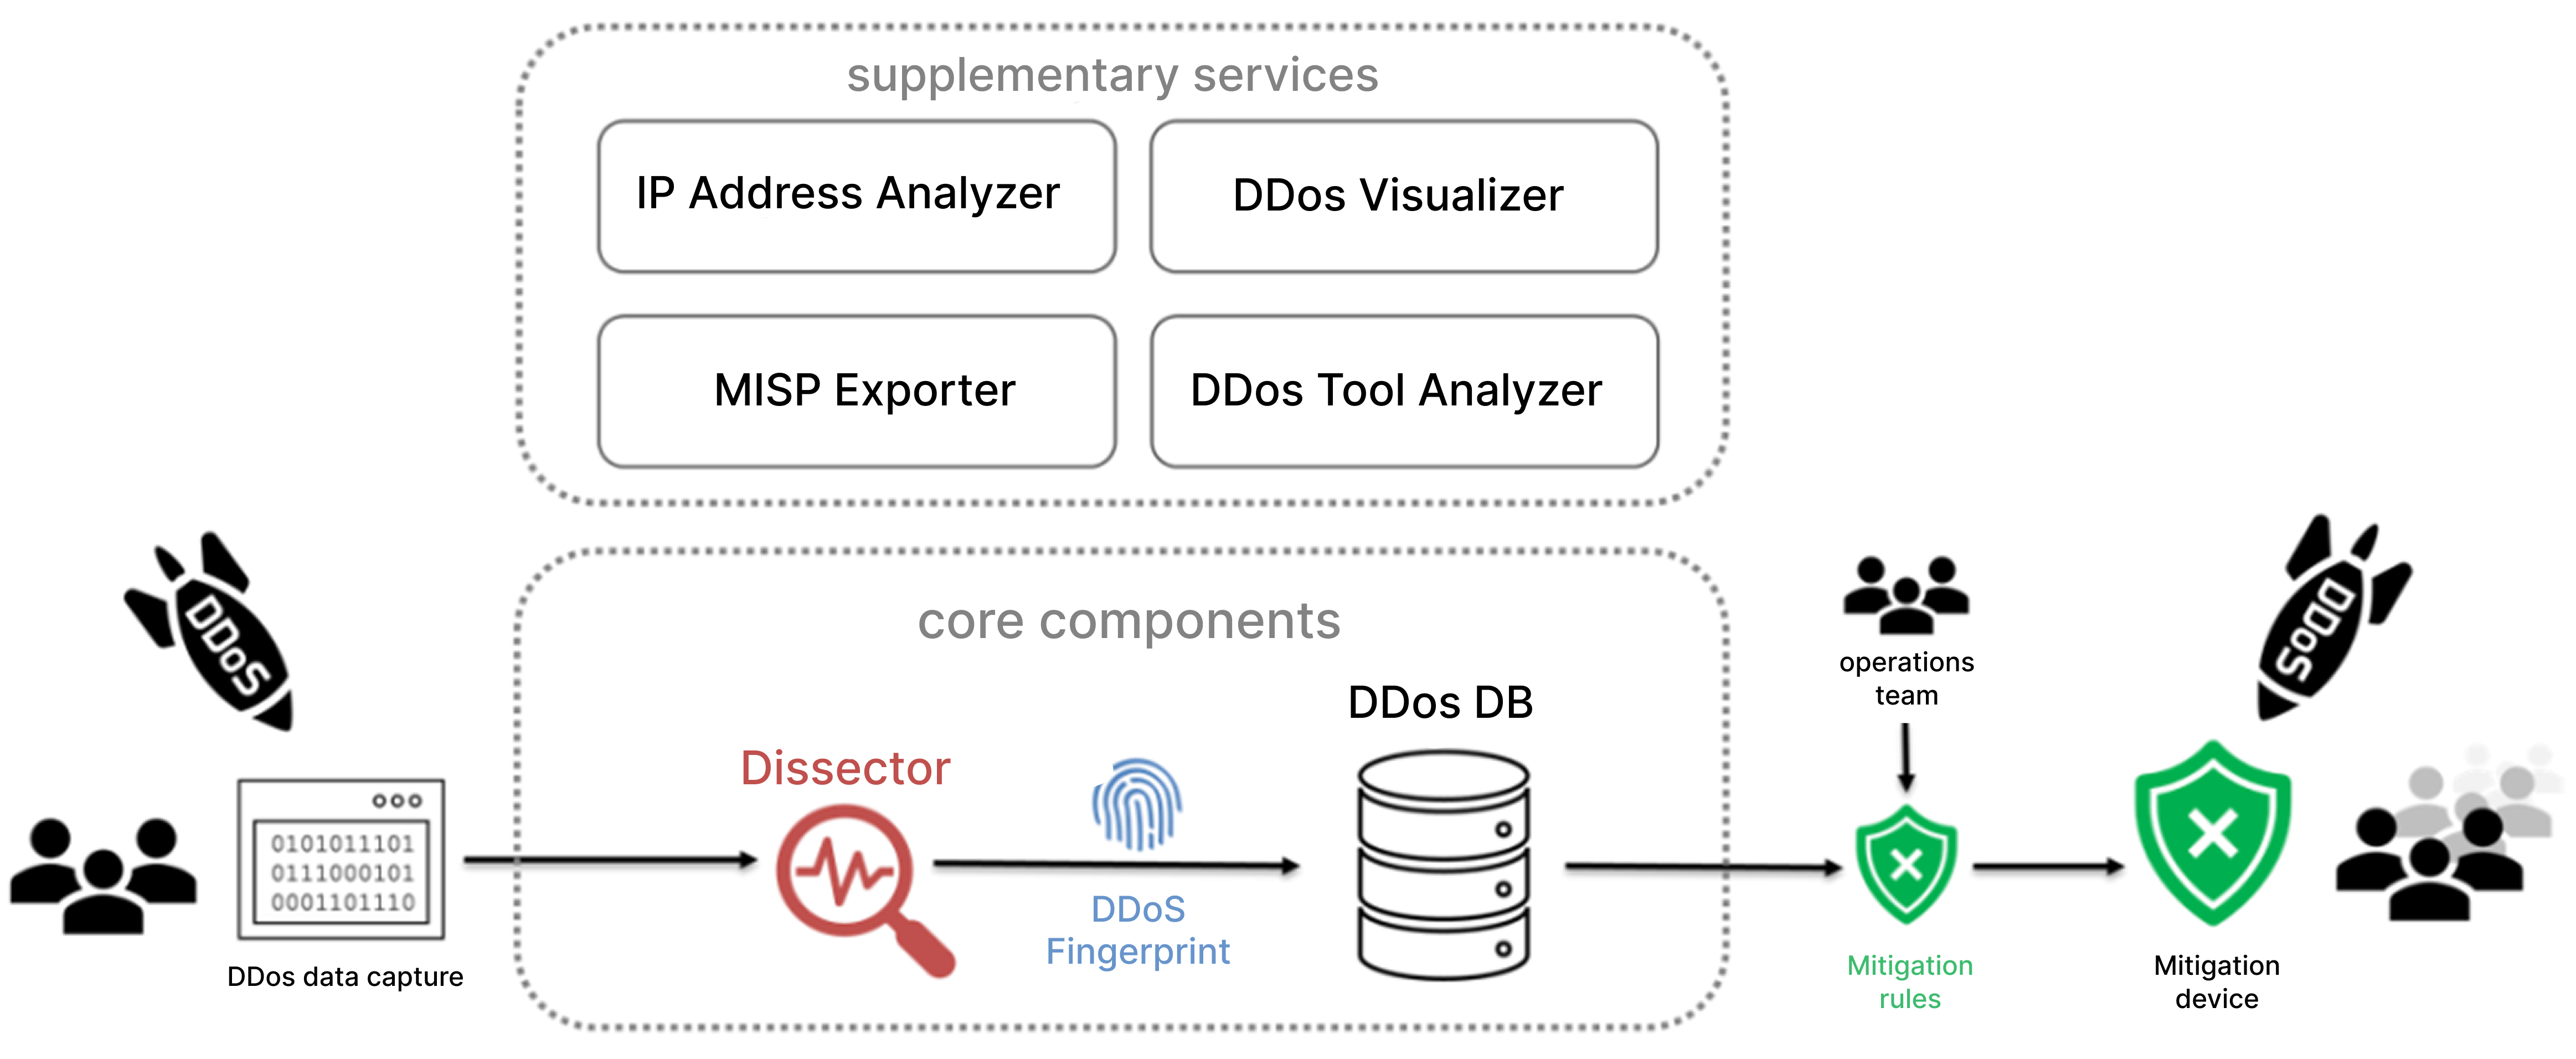
\includegraphics[width=1\textwidth]{clearing_house.png}


\caption{Architecture du \textit{DDoS Clearing House} : génération d'empreintes DDoS par le composant Dissector, stockage dans la base DDoS DB, puis utilisation par l'équipe opérationnelle pour générer des règles de mitigation.}

\label{fig:ddos_clearing_house}

\end{figure}

\subsection{Limites identifiées}

\begin{itemize}
    \item \textbf{Partage passif sans orchestration~:} Le système se limite au partage d'\textbf{intelligence} (\textit{Threat Intel}) sans orchestrer de réponse active. Il n'y a pas de mécanisme pour qu'un membre demande une mitigation distribuée aux autres --- chaque membre applique indépendamment les règles dérivées des fingerprints reçus.

    \item \textbf{Architecture centralisée (\gls{spof})~:} Le hub central constitue un point de défaillance unique~: s'il est indisponible (panne, attaque ciblée), la dissémination des fingerprints est interrompue. La déduplique et l'enrichissement dépendent entièrement de ce composant.

    \item \textbf{Partage \textit{a posteriori}~:} La génération d'un fingerprint nécessite l'analyse du trafic d'attaque \textit{après} sa détection. Le temps de traitement (capture PCAP $\rightarrow$ extraction DissecTor $\rightarrow$ upload API $\rightarrow$ déduplique $\rightarrow$ download par les membres $\rightarrow$ conversion en règles) introduit un \textbf{délai incompressible de l'ordre de plusieurs minutes} \cite{sidnlabs2021clearinghouse}, rendant le système inefficace contre les attaques éphémères (\textit{hit-and-run}, durée $<$~5~min).

    \item \textbf{Confiance implicite~:} Le système ne définit pas de mécanisme formel de vérification de la véracité d'un fingerprint soumis. Un membre compromis ou malveillant pourrait théoriquement injecter de faux fingerprints pour provoquer le blocage de trafic légitime chez les autres membres (\textit{poisoning attack}).
\end{itemize}

% --------------------------------------------------
\section{NaWas / NBIP --- Centre national de \textit{scrubbing} mutualisé}
\label{sec:nawas}

\subsection{Contexte et architecture}

NaWas (\textit{National Wasstraat}, littéralement \og station de lavage nationale \fg{}) est une initiative néerlandaise opérée par le NBIP (\textit{Nationale Beheersorganisatie Internet Providers}), un consortium à but non lucratif regroupant des \glspl{fai} néerlandais. Elle offre une infrastructure de \textit{scrubbing} mutualisée aux membres participants \cite{nbip2023nawas}.

\subsubsection{Mécanisme de redirection BGP}

L'activation de la protection NaWas repose sur le principe de l'\textbf{injection de routes plus spécifiques} via \gls{bgp}. En cas d'attaque (voir Figure~\ref{fig:nawas_bgp})~:

\begin{enumerate}
    \item Le membre annonce le préfixe IP attaqué (ex.~: \texttt{203.0.113.0/24}) à la plateforme NaWas via une session eBGP dédiée, en y attachant une \textbf{communauté BGP spécifique} (ex.~: \texttt{AS:666} ou une communauté étendue propriétaire) qui indique la demande de scrubbing.

    \item NaWas \textbf{réannonce} ce préfixe vers ses fournisseurs de transit (\textit{upstream providers}) avec un \textit{AS-path} plus court, attirant ainsi le trafic destiné au préfixe attaqué (\textit{traffic attraction} par spécificité de préfixe).

    \item Le trafic entrant est traité par des \textbf{\textit{scrubbing lanes}} (lignes de nettoyage) composées d'appliances matérielles et logicielles qui appliquent~:
    \begin{itemize}
        \item Un \textbf{filtrage basé sur signatures} (\gls{dpi}) pour les vecteurs d'attaque connus.
        \item Un \textbf{\textit{rate limiting}} adaptatif par source IP et par protocole.
        \item Une \textbf{analyse comportementale} (détection d'anomalies statistiques sur la distribution des tailles de paquets, TTL, flags TCP).
        \item Un \textbf{challenge cryptographique} (SYN cookies, JavaScript challenge pour HTTP) pour valider les connexions légitimes.
    \end{itemize}

    \item Le trafic nettoyé (\textit{clean traffic}) est renvoyé au membre via un \textbf{tunnel \gls{gre}} (RFC~2784) ou un \textbf{VLAN dédié} sur une interconnexion privée, contournant ainsi la saturation des liens publics du membre. Le routage de retour utilise un chemin distinct (\textit{clean-return path}) pour éviter les boucles de routage.
\end{enumerate}

\begin{figure}[htbp]
\centering
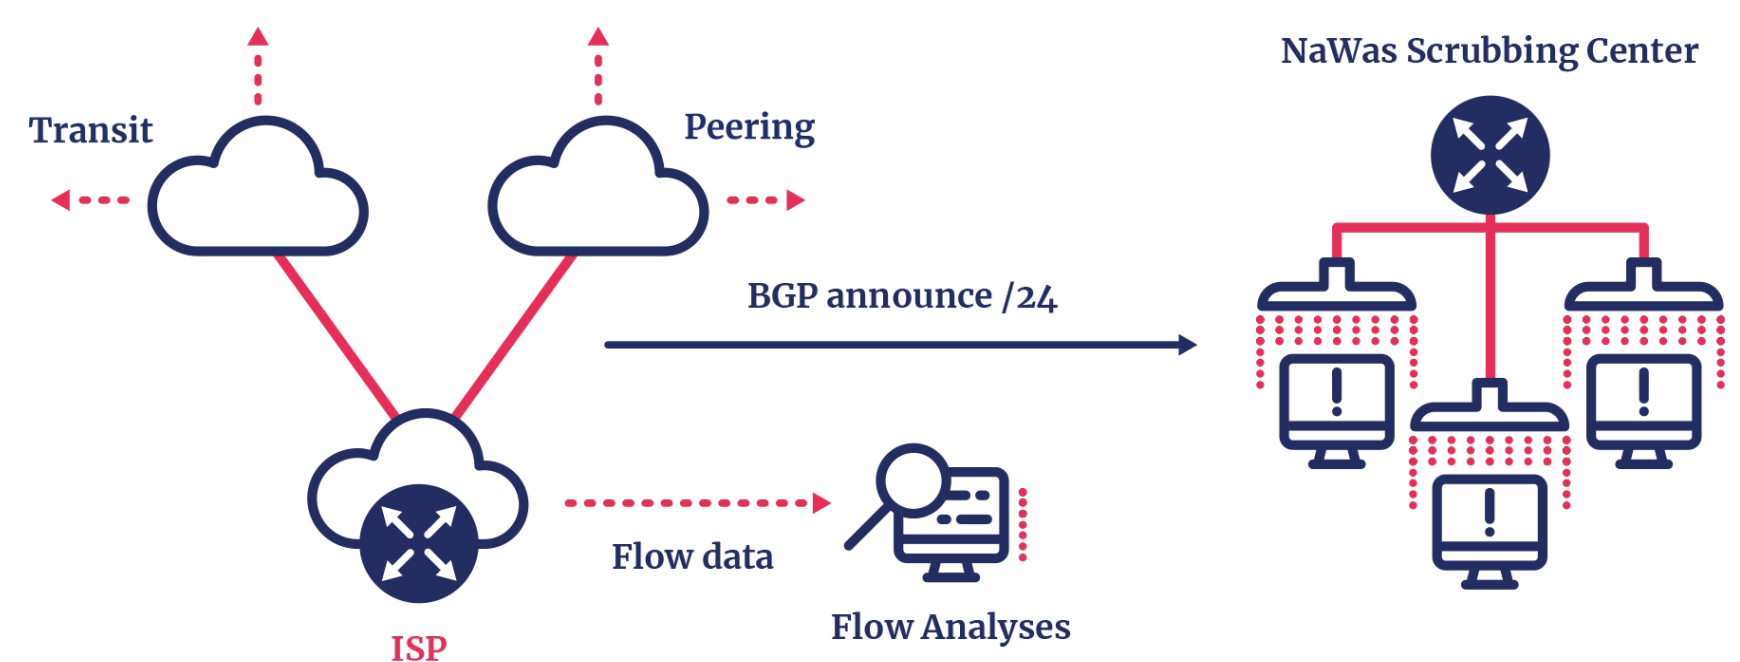
\includegraphics[width=0.85\textwidth]{nawas.png}

\caption{Architecture simplifiée du service NaWas : redirection du trafic vers un centre de scrubbing mutualisé via annonce BGP et analyse des flux avant application des mécanismes de mitigation.}

\label{fig:nawas_bgp}
\end{figure}

\subsection{Limites identifiées}

\begin{itemize}
    \item \textbf{Architecture semi-centralisée~:} Bien que mutualisée, l'infrastructure physique de NaWas est centralisée aux Pays-Bas (quelques PoP sur des IXP néerlandais --- AMS-IX, NL-ix). Un membre éloigné géographiquement subit une latence de redirection significative. Le \textit{scrubbing center} lui-même peut devenir un \gls{spof} en cas d'attaque ciblant directement l'infrastructure NaWas.

    \item \textbf{Activation semi-manuelle~:} L'injection de la route \gls{bgp} avec la communauté de scrubbing nécessite typiquement une \textbf{intervention de l'opérateur} du membre (commande CLI sur le routeur de bordure ou via un portail web). Il n'y a pas de mécanisme de détection et d'activation entièrement automatisé intégré au protocole --- l'automatisation dépend de l'intégration locale chez chaque membre.

    \item \textbf{Absence de coordination horizontale inter-membres~:} Les membres NaWas n'échangent pas de métadonnées d'attaque entre eux ni ne coordonnent leurs actions de filtrage. Chaque membre interagit uniquement avec la plateforme centrale. Il n'y a pas de partage d'intelligence comparable au Clearing House.

    \item \textbf{Capacité finie~:} La capacité totale de scrubbing est dimensionnée pour le volume agrégé moyen des attaques ciblant les membres. En cas d'attaque volumétrique massive ($>$~1~Tbps) ciblant un seul membre, la capacité mutualisée peut être insuffisante sans mécanisme de débordement (\textit{overflow}) vers des tiers.
\end{itemize}

% --------------------------------------------------
\section{DefCOM --- \textit{Distributed Cooperative Overlay Defense}}
\label{sec:defcom}

\subsection{Contexte et architecture}

Proposé par Mirkovic et al. \cite{mirkovic2003defcom}, DefCOM est un système de défense coopérative qui structure les n\oe{}uds de défense en un \textbf{réseau overlay logique} pour éviter les goulots d'étranglement centraux. C'est l'une des premières propositions académiques de défense \gls{ddos} véritablement distribuée.

\subsubsection{Topologie et rôles des n\oe{}uds}

DefCOM définit trois rôles fonctionnels pour les n\oe{}uds participants~:
\begin{itemize}
    \item \textbf{N\oe{}uds \textit{Victim-end} (V-nodes)~:} Déployés dans le réseau de la victime, ils \textbf{détectent} l'attaque en observant la surcharge locale (taux d'utilisation CPU, bande passante saturée, taux de paquets rejetés) et \textbf{initient} la réponse coopérative en classifiant les flux entrants comme légitimes (\textit{good}) ou suspects (\textit{bad}) à l'aide de statistiques locales et de listes blanches préétablies.

    \item \textbf{N\oe{}uds \textit{Core} (C-nodes)~:} Positionnés dans les réseaux intermédiaires (\glspl{fai} de transit), ils relayent les informations de contrôle et appliquent le \textbf{\textit{rate limiting}} sur les flux signalés comme suspects. Chaque C-node maintient un \textbf{classifieur de paquets} qui marque les paquets traversants via un champ de l'en-tête IP pour distinguer le trafic légitime du trafic suspect en aval.

    \item \textbf{N\oe{}uds \textit{Source-end} (S-nodes)~:} Déployés au plus proche des sources d'attaque, ils appliquent le filtrage le plus agressif sur les flux identifiés comme malveillants, en utilisant les informations reçues des V-nodes et C-nodes. Leur objectif est de \textbf{supprimer le trafic d'attaque au plus tôt} dans le chemin réseau, préservant ainsi la bande passante des liens intermédiaires.
\end{itemize}

\subsubsection{Mécanisme de \textit{Rate Limiting} coopératif}

L'architecture met en \oe{}uvre un mécanisme de \textbf{\textit{Rate Limiting} coopératif hiérarchique} (voir Figure~\ref{fig:defcom_tree}). Le protocole fonctionne comme suit~:

\begin{enumerate}
    \item Le V-node détecte une surcharge et calcule un \textbf{débit maximal acceptable} ($R_{max}$) pour le trafic entrant sur le préfixe attaqué.

    \item Il envoie un message de type \texttt{RATE\_LIMIT\_REQUEST} à ses C-nodes voisins dans l'overlay, contenant~: le préfixe cible, le débit maximal $R_{max}$, et une liste de préfixes sources classés comme suspects.

    \item Chaque C-node recevant ce message \textbf{répartit} la limite de débit $R_{max}$ proportionnellement entre ses liens amont~:
    \begin{equation}
        R_i = R_{max} \times w_i
        \label{eq:rate_limit}
    \end{equation}
    où $w_i$ est le poids du lien $i$ basé sur le volume de trafic observé, puis propage la demande vers les n\oe{}uds plus en amont.

    \item Ce processus forme un \textbf{arbre de limitation de débit} (\textit{rate-limiting tree}) où la contrainte se propage de la victime vers les sources, chaque n\oe{}ud intermédiaire appliquant sa part du budget de débit.

    \item Les S-nodes, en bout de chaîne, appliquent le \textbf{filtrage terminal}~: les flux dépassant leur budget alloué $R_i$ sont soit rejetés (\textit{drop}), soit soumis à un marquage probabiliste (\textit{probabilistic drop}) privilégiant les sources connues comme légitimes.
\end{enumerate}

\subsubsection{Protocole de communication overlay}

La communication entre les n\oe{}uds se fait via un \textbf{protocole de type \textit{gossip}} (épidémique). Chaque n\oe{}ud maintient une \textbf{table de voisinage} (liste de pairs connus) et diffuse périodiquement ses informations d'état (charge actuelle, débit traité, alertes actives) à un sous-ensemble aléatoire de ses voisins. Ce mécanisme assure~:
\begin{itemize}
    \item Une \textbf{convergence rapide}~: l'information atteint tous les n\oe{}uds en $O(\log N)$ rounds de gossip pour $N$ participants.
    \item Une \textbf{tolérance aux pannes}~: la perte d'un n\oe{}ud intermédiaire n'empêche pas la propagation, grâce à la redondance des chemins de diffusion.
\end{itemize}

La construction de l'overlay suit un mécanisme de \textbf{découverte initiale par traceroute}~: chaque n\oe{}ud participant exécute des \texttt{traceroute} vers les autres n\oe{}uds connus pour reconstruire la topologie Internet sous-jacente et positionner correctement les C-nodes sur le chemin entre sources et victimes.

\begin{figure}[htbp]
    \centering
     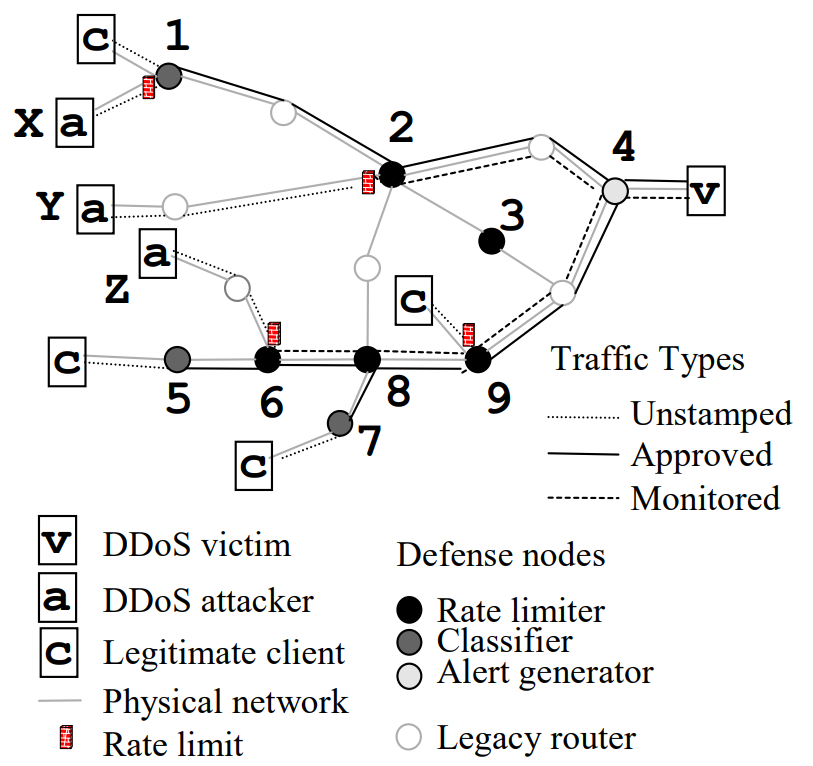
\includegraphics[width=0.75\textwidth]{defcom.png}
 
    \caption{Arbre de limitation de débit coopératif dans DefCOM~: propagation de la demande de la victime vers les sources.}
    \label{fig:defcom_tree}
\end{figure}

\subsection{Limites identifiées}

\begin{itemize}
    \item \textbf{Contribution purement académique~:} DefCOM est resté au stade de prototype évalué en simulation (ns-2). Aucun déploiement opérationnel à grande échelle n'a été documenté. Les évaluations publiées portent sur des topologies simulées de quelques dizaines de n\oe{}uds, loin des conditions réelles de l'Internet.

    \item \textbf{Absence de standards d'interopérabilité~:} Le protocole de communication overlay (format des messages, encodage, machine à états) n'est défini que dans les publications académiques, sans spécification formelle (pas de RFC, pas de schéma YANG, pas d'API standardisée). Cela rend l'interopérabilité entre implémentations différentes impossible en pratique.

    \item \textbf{Vulnérabilité aux n\oe{}uds compromis~:} Le modèle de confiance de DefCOM est \textbf{implicite}~: tout n\oe{}ud participant est considéré comme honnête. Un n\oe{}ud compromis pourrait~:
    \begin{itemize}
        \item Générer de \textbf{fausses alertes} (\texttt{RATE\_LIMIT\_REQUEST} avec des préfixes légitimes comme cibles) pour provoquer le blocage de trafic légitime (\textit{blackholing} offensif).
        \item \textbf{Ignorer} les demandes de \textit{rate limiting} reçues (\textit{free-riding}).
        \item \textbf{Manipuler} les poids de répartition pour rediriger le trafic légitime vers des liens saturés.
    \end{itemize}
    Aucun mécanisme de \textbf{réputation}, de \textbf{vérification cryptographique des messages}, ou de \textbf{détection de comportement byzantin} n'est intégré.

    \item \textbf{Hypothèse de déploiement incrémental~:} DefCOM suppose un \textbf{déploiement coopératif} par des \glspl{as} multiples, incluant des \glspl{fai} de transit. En pratique, l'incitation économique pour un \gls{fai} de transit à déployer un n\oe{}ud DefCOM (qui consomme des ressources pour protéger les clients d'un autre \gls{as}) est faible, posant un problème classique d'\textbf{externalité} en économie des réseaux.

    \item \textbf{Scalabilité de la découverte par traceroute~:} La reconstruction de la topologie overlay via \texttt{traceroute} génère un volume de trafic de sondage quadratique ($O(N^2)$ pour $N$ n\oe{}uds) et les résultats sont instables (asymétrie de routage, filtrage ICMP, load balancing).
\end{itemize}

% --------------------------------------------------
\section{Synthèse comparative}
\label{sec:synthese}

Le Tableau~\ref{tab:comparaison} compare les travaux analysés selon les critères clés de la coordination distribuée anti-\gls{ddos}.


\begin{table}[htbp]
\centering
\small
\renewcommand{\arraystretch}{1.3}

\resizebox{\textwidth}{!}{
\begin{tabular}{|l|l|c|c|c|c|}
\hline
\textbf{Système} & \textbf{Architecture} & \textbf{P2P} & \textbf{Partage méta.} & \textbf{Sync. actions} & \textbf{Mutualisation} \\
\hline
\gls{dots} (RFC~8612) & Client-serveur & $\times$ & $\checkmark$ (partiel) & $\checkmark$ & $\times$ \\
\hline
DDoS Clearing House & Centralisée & $\times$ & $\checkmark$ & $\times$ & $\times$ \\
\hline
NaWas / NBIP & Semi-centralisée & $\times$ & $\times$ & $\times$ & $\checkmark$ \\
\hline
DefCOM & P2P overlay & $\checkmark$ & $\checkmark$ (partiel) & $\checkmark$ (partiel) & $\times$ \\
\hline
\end{tabular}
}

\caption{Comparaison des systèmes de défense collaborative contre les attaques DDoS.}
\label{tab:comparaison}

\end{table}

L'analyse révèle qu'aucun système existant ne combine simultanément~:
\begin{enumerate}
    \item Une architecture \textbf{véritablement décentralisée} (\gls{p2p}) éliminant tout \gls{spof}.
    \item Un mécanisme de \textbf{partage de métadonnées d'attaque en temps réel} (et non \textit{a posteriori}).
    \item Une \textbf{orchestration coordonnée des actions de mitigation} entre les n\oe{}uds participants.
    \item Un \textbf{modèle de confiance dynamique} permettant de vérifier la fiabilité des pairs sans relation préétablie.
    \item Une \textbf{mutualisation effective des capacités} de scrubbing entre n\oe{}uds.
\end{enumerate}

% --------------------------------------------------
\section{Conclusion}

L'Étude bibliographique révèle une progression vers la défense collaborative~: \gls{dots} standardise la signalisation inter-domaines mais reste hiérarchique~; le Clearing House partage l'intelligence d'attaque mais sans orchestration active et avec un délai inhérent~; NaWas mutualise les ressources physiques mais sans coordination horizontale entre membres~; DefCOM propose une architecture overlay distribuée mais manque de mécanismes de confiance et d'interopérabilité.

\textbf{Aucun système ne combine pleinement} une architecture décentralisée (\gls{p2p}), une coordination d'actions en temps réel, un partage d'intelligence proactif et des mécanismes de confiance robustes. C'est précisément dans cet espace que s'inscrit la contribution présentée dans les chapitres suivants de ce mémoire.
% =============================================
% CHAPITRE 3 : Conception et Architecture du système
% =============================================
\chapter{Conception et Architecture du système}
\label{chap:conception}

\section{Introduction}

Les chapitres précédents ont mis en évidence deux constats~: les attaques \gls{ddos} modernes dépassent les capacités de défense individuelles, et les systèmes collaboratifs existants souffrent d'une centralisation résiduelle ou d'une absence de mécanisme de confiance formalisé. Ce chapitre présente la conception du système distribué de mitigation collaborative qui répond à ces lacunes.

Il est organisé en deux parties~: la \textbf{conception préliminaire} établit les exigences et l'architecture globale du système~; la \textbf{conception technique détaillée} formalise les modèles de données, les algorithmes et les protocoles de sécurité retenus.

% ==================================================
\section{Conception préliminaire}
\label{sec:conception_prelim}
% ==================================================

\subsection{Architecture générale}
\label{sec:architecture_gen}

\subsubsection{Topologie de la coalition}
La solution proposée adopte une architecture \gls{p2p} non structurée, dans laquelle chaque nœud maintient localement un registre des pairs qu'il connaît. Ce choix repose sur trois motivations principales. Premièrement, les participants de la coalition présentent une forte hétérogénéité en termes de ressources et de capacités ; une architecture plate permet ainsi d'éviter la désignation arbitraire de nœuds privilégiés ou de points de concentration. Deuxièmement, cette approche renforce la résilience du système : la défaillance ou le retrait d'un pair n'entraîne pas l'interruption du fonctionnement global du réseau, aucun nœud ne constituant un point central de dépendance. Enfin, elle favorise l'évolutivité de la coalition : de nouveaux participants peuvent rejoindre le réseau sans nécessiter de reconfiguration globale ni de coordination centralisée, permettant ainsi à l'infrastructure de s'adapter progressivement à l'augmentation du nombre de membres \cite{lua2005survey}.

\begin{figure}[H]
\centering
\begin{tikzpicture}[
    pair/.style={
        circle, draw, thick,
        minimum size=1.8cm,
        align=center, font=\small
    },
    lien/.style={<->, thick, gray!60}
]
\node[pair, fill=white]    (A) at (0,3.5)     {Pair A\\Université};
\node[pair, fill=white]   (B) at (4,4)       {Pair B\\Datacenter};
\node[pair, fill=white]  (C) at (7,1.5)     {Pair C\\FAI};
\node[pair, fill=white]  (D) at (5,-1.5)    {Pair D\\PME};
\node[pair, fill=white]     (E) at (1.5,-2)    {Pair E\\Gouvernement};
\node[pair, fill=white]  (F) at (-2,1)      {Pair F\\Université};
\node[pair, fill=white]    (G) at (2.5,1.5)   {Pair G\\Recherche};

\draw[lien] (A) -- (B);
\draw[lien] (B) -- (C);
\draw[lien] (C) -- (D);
\draw[lien] (D) -- (E);
\draw[lien] (E) -- (F);
\draw[lien] (F) -- (A);
\draw[lien] (A) -- (G);
\draw[lien] (B) -- (G);
\draw[lien] (G) -- (D);
\draw[lien] (G) -- (E);
\draw[lien] (F) -- (G);
\draw[lien] (C) -- (G);
\end{tikzpicture}
\caption{Exemple de coalition~: sept nœuds hétérogènes interconnectés en overlay \gls{p2p} plat non structuré.}
\label{fig:coalition}
\end{figure}

\subsubsection{Cycle de vie d'une session de mitigation}
\label{subsec:cycle_vie}

Le flux d'une session d'aide suit quatre phases distinctes~:

\begin{enumerate}
    \item \textbf{Détection et escalade~:} le nœud victime détecte un débordement de capacité et diffuse une demande d'aide à l'ensemble des membres actifs de la coalition, sans présélection ni allocation préalable.
    \item \textbf{Négociation~:} les pairs reçoivent la demande d'aide et acceptent ou rejettent en fonction de leur capacité disponible~; en cas d'acceptation, chaque pair déclare lui-même le volume qu'il peut offrir.
    \item \textbf{Allocation~:} une fois les réponses connues, le nœud victime calcule par l'algorithme WSM la répartition optimale du flux excédentaire parmi les seuls pairs ayant accepté.
    \item \textbf{Redirection active~:} le trafic excédentaire est redirigé vers les pairs acceptants via un tunnel (GRE, VXLAN ou IPIP), selon le plan d'allocation calculé.
    \item \textbf{Clôture~:} à la fin de l'attaque, le nœud victime notifie la clôture ({POST /attack/over}), capture les crédibilités réseau au moment de la session et recalcule les scores de confiance.
\end{enumerate}

\subsection{Périmètre du système}
\label{subsec:perimetre_redirection}

La Figure~\ref{fig:archi_redirection} présente l'architecture globale du système 
et délimite explicitement son périmètre. Le système gère l'intégralité de la 
coordination applicative~: diffusion des demandes d'aide \textbf{(1)}, collecte 
des réponses des pairs acceptants ou refusants \textbf{(2)} et émission du signal 
de redirection \textbf{(3)}. En revanche, la redirection physique du trafic reste 
hors périmètre et repose sur l'infrastructure réseau du nœud victime~: c'est elle qui achemine le trafic excédentaire vers les 
pairs aidants \textbf{(4)}, lesquels filtrent le trafic malveillant et renvoient 
le trafic propre vers cette même infrastructure \textbf{(5)}, avant qu'il ne soit 
agrégé et retransmis au nœud victime \textbf{(6)}.

\begin{figure}[H]
\centering
\figborder[\textwidth]{figures/archi_redirection.pdf}
\caption{Architecture globale du système ShieldNet~: périmètre applicatif et redirection réseau hors périmètre.}
\label{fig:archi_redirection}
\end{figure}

\subsection{Diagrammes de cas d'utilisation}
\label{subsec:uc}

Le système est décrit par trois diagrammes de cas d'utilisation complémentaires, couvrant respectivement le protocole de mitigation collaborative, le moteur de confiance PeerTrust et le rôle complet du nœud pair dans la coalition. Les trois acteurs impliqués sont~: le \textbf{nœud local} (victime en situation d'attaque) et le \textbf{nœud pair} (participant distant).
%et l'\textbf{administrateur} (responsable de la configuration locale).

% --------------------------------------------------
\subsubsection{Protocole de mitigation collaborative}
% --------------------------------------------------
La Figure~\ref{fig:uc_mitigation} détaille les interactions entre le nœud victime 
et le nœud pair lors d'une session de mitigation. Ce diagramme couvre le flux complet 
depuis l'envoi de la demande d'aide jusqu'au recalcul du score de confiance.

Le nœud victime initie la séquence en diffusant une demande d'aide à l'ensemble
des pairs actifs de la coalition, sans présélection ni allocation préalable.
Chaque nœud pair sollicité peut alors accepter ou rejeter la session ; en cas
d'acceptation, il déclare lui-même la capacité qu'il peut offrir. Une fois les
réponses connues, le nœud victime calcule la répartition optimale du flux parmi
les seuls pairs ayant accepté, via l'algorithme WSM : chaque pair accepteur est
évalué selon quatre critères pondérés (capacité déclarée à l'acceptation, latence
inversée, score de confiance et réciprocité). L'acceptation déclenche ensuite
l'activation de la mitigation, qui correspond au signal de démarrage de la
redirection au niveau applicatif. La clôture de l'attaque, initiée par le nœud
victime, inclut deux actions systématiques : la mise à jour des crédits de
réciprocité des deux nœuds dans leurs registres respectifs, et le recalcul du
score de confiance PeerTrust $T(u)$ du pair assistant.

\begin{figure}[H]
\centering
\figborder[\textwidth]{figures/uc_mitigation_collaborative1.pdf}

\caption{Diagramme de cas d'utilisation~: Protocole de mitigation collaborative.}
\label{fig:uc_mitigation}
\end{figure}

% --------------------------------------------------
\subsubsection{Moteur de confiance PeerTrust}
% --------------------------------------------------
La figure~\ref{fig:uc_trust} présente les cas d'utilisation du moteur
de confiance. L'acteur unique est le nœud local, qui peut
déclencher le recalcul du score à la clôture d'une session d'aide,
consulter le score d'un pair, ou forcer un recalcul manuel. Le
bannissement automatique est déclenché lorsque le score calculé
est inférieur à $0{,}20$, ou suite à la détection d'une violation
de comportement.


\begin{figure}[H]
\centering
\figborder[\textwidth]{figures/uc_moteur_confiance.pdf}
\caption{Diagramme de cas d'utilisation~: Moteur de confiance PeerTrust.}
\label{fig:uc_trust}
\end{figure}

% --------------------------------------------------
\subsubsection{Rôle du nœud pair dans la coalition}
% --------------------------------------------------

La Figure~\ref{fig:uc_pair} présente l'ensemble des actions qu'un \textbf{nœud pair} peut effectuer au sein de la coalition, organisées en quatre groupes fonctionnels.

Le groupe \textbf{Membership} couvre le cycle de vie complet du pair~: il s'enregistre, action qui inclut obligatoirement la publication de ses capacités de scrubbing; il peut ensuite découvrir des pairs disponibles et consulter la liste des pairs connus; il diffuse un heartbeat sur événement (adhésion, mise à jour de paramètres ou départ) pour signaler sa disponibilité et mettre à jour sa capacité déclarée~; enfin, il peut quitter proprement la coalition, ce qui met son statut à {INACTIVE} ou {MAINTENANCE}.

Le groupe \textbf{Session d'aide} couvre les deux modes de participation~: le pair peut recevoir une requête d'aide  et choisir de l'accepter  ou de la rejeter , ou bien proposer proactivement de l'aide  lorsque le flag {auto\_offer\_enabled} est activé dans sa politique locale~; une offre acceptée étend vers le même cas d'usage Accepter la session d'aide.

Le groupe \textbf{Confiance} contient un seul cas d'usage~: interroger la coalition sur sa réputation, qui correspond à la collecte de la crédibilité $Cr$ utilisée dans la formule PeerTrust.

Le groupe \textbf{Sécurité} couvre l'obtention d'un token, prérequis à tout appel API authentifié.

\begin{figure}[H]
\centering
\figborder[\textwidth]{figures/uc_role_pair.pdf}
\caption{Diagramme de cas d'utilisation~: Rôle du nœud pair dans la coalition (12 cas d'usage).}
\label{fig:uc_pair}
\end{figure}

% --------------------------------------------------
\subsection{Documentation des cas d'utilisation}
\label{subsec:cu_doc}
% --------------------------------------------------

Les tableaux suivants documentent les six principaux cas d'utilisation du système, issus des trois diagrammes présentés ci-dessus. Le Tableau~\ref{tab:cu_identification} en présente la synthèse.

\begin{comment}
\begin{table}[H]
\centering
\caption{Identification des cas d'utilisation.}
\label{tab:cu_identification}
\small
\renewcommand{\arraystretch}{1.35}
\begin{tabularx}{\textwidth}{|c|l|l|X|}
\hline
\textbf{ID} & \textbf{Nom} & \textbf{Acteur principal} & \textbf{Description courte} \\
\hline
CU~1 & Obtenir un token JWT RS256      & Nœud local / pair      & Authentification auprès de l'API via une clé privée RS256~; token valable 15~minutes. \\
\hline
CU~3 & Envoyer un heartbeat            & Nœud pair              & Signal périodique (30~s) transmettant la charge et la capacité disponible. \\
\hline
CU~4 & Envoyer une requête d'aide      & Nœud victime           & Sélection WSM des pairs et envoi de {POST /help/request}. \\
\hline
CU~5 & Accepter ou rejeter une session & Nœud pair              & Réponse à une requête d'aide selon la capacité disponible. \\
\hline
CU~6 & Clôturer l'attaque              & Nœud victime           & Fermeture des sessions, mise à jour des crédits et recalcul PeerTrust. \\
\hline
CU~7 & Recalculer le score PeerTrust   & Moteur de confiance    & Calcul de $T(u)$ et bannissement automatique si $T(u) < 0{,}20$. \\
\hline
\end{tabularx}
\end{table}
\end{comment}


\begin{table}[H]
\centering
\caption{Identification des cas d'utilisation.}
\label{tab:cu_identification}

\renewcommand{\arraystretch}{1.8}
\setlength{\tabcolsep}{5pt}

\begin{tabular}{|
>{\raggedright\arraybackslash}p{1.2cm}|
>{\raggedright\arraybackslash}p{3.5cm}|
>{\raggedright\arraybackslash}p{3.0cm}|
>{\raggedright\arraybackslash}p{5.0cm}|}
\hline

\textbf{ID} &
\textbf{Nom} &
\textbf{Acteur principal} &
\textbf{Description courte} \\
\hline

CU~1 &
Obtenir un token JWT RS256 &
Nœud local / pair &
Authentification auprès de l'API via une clé privée RS256 ; token valable 15~m. \\
\hline

CU~3 &
Envoyer un heartbeat &
Nœud pair &
Signal événementiel (adhésion, mise à jour ou départ) transmettant la charge et la capacité disponible. \\
\hline

CU~4 &
Envoyer une requête d'aide &
Nœud victime &
Sollicitation diffusée à tous les pairs actifs, sans allocation préalable. \\
\hline

CU~5 &
Accepter ou rejeter une session &
Nœud pair &
Réponse à une requête d'aide, avec déclaration de la capacité offerte. \\
\hline

CU~5bis &
Calculer l'allocation WSM &
Nœud victime &
Répartition optimale du flux entre les pairs ayant accepté. \\
\hline

CU~6 &
Clôturer l'attaque &
Nœud victime &
Fermeture des sessions, mise à jour des crédits et recalcul PeerTrust. \\
\hline

CU~7 &
Recalculer le score PeerTrust &
Moteur de confiance &
Calcul de $T(u)$ et bannissement automatique si $T(u) < 0{,}20$. \\
\hline

\end{tabular}

\end{table}



% ─── CU 1 ─────────────────────────────────────────────────────────────────────
\begin{table}[H]
\centering
\renewcommand{\arraystretch}{1.5}
\begin{tabular}{|p{3.5cm}|p{10.5cm}|}
\hline
\multicolumn{2}{|c|}{\textbf{CU~1 : Obtenir un token JWT RS256}} \\
\hline
\textbf{ID} & 1 \\
\hline
\textbf{Description} & Le nœud (local ou pair) demande un token JWT signé RS256 afin d'accéder aux routes protégées de l'API. Le token est valide exactement 15~minutes. \\
\hline
\textbf{Acteurs primaires} & Nœud local, nœud pair \\
\hline
\textbf{Acteurs secondaires} & Module d'authentification (composant interne du nœud cible) \\
\hline
\textbf{Préconditions} & La clé privée RSA du nœud ({node.key}) est présente sur le système de fichiers. \\
\hline
\textbf{Enchaînement principal} &
Ce CU démarre lorsque le nœud doit appeler une route protégée de l'API.\newline
\textbf{1.}\ Le nœud envoie {POST /api/v1/auth/token} avec son identifiant ({node\_id}).\newline
\textbf{2.}\ Le module d'authentification lit la clé privée RS256 stockée localement ({node.key}).\newline
\textbf{3.}\ Le système génère un JWT signé contenant {\{iss, node\_id, iat, exp\}} avec une durée de vie de 15~minutes.\newline
\textbf{4.}\ Le token est retourné au nœud appelant (HTTP~200).\newline
\textbf{5.}\ Le nœud inclut ce token dans l'en-tête {Authorization: Bearer <token>} pour toutes ses requêtes suivantes. \\
\hline
\textbf{Post-conditions} & Le nœud dispose d'un token RS256 valide pour 15~minutes. \\
\hline
\textbf{Enchaînements alternatifs} &
\textbf{Clé privée introuvable~:} le serveur retourne HTTP~500.\newline
\textbf{Token expiré lors d'un appel ultérieur~:} le serveur retourne HTTP~401 ; le nœud doit redemander un token via ce même CU. \\
\hline
\end{tabular}
\caption{Documentation du cas d'utilisation \textit{Obtenir un token JWT RS256}.}
\label{tab:cu1}
\end{table}


% ─── CU 3 ─────────────────────────────────────────────────────────────────────
\begin{table}[H]
\centering
\renewcommand{\arraystretch}{1.5}
\begin{tabular}{|p{3.5cm}|p{10.5cm}|}
\hline
\multicolumn{2}{|c|}{\textbf{CU~3 : Envoyer un heartbeat}} \\
\hline
\textbf{ID} & 3 \\
\hline
\textbf{Description} & Un nœud pair signale sa disponibilité et met à jour sa capacité déclarée auprès de ses pairs connus, sur événement uniquement~: aucun minuteur périodique n'envoie de signal en l'absence de changement. \\
\hline
\textbf{Acteurs primaires} & Nœud pair \\
\hline
\textbf{Acteurs secondaires} & Nœuds pairs connus (registres distants de la coalition) \\
\hline
\textbf{Préconditions} & Le nœud pair est enregistré (statut \texttt{ACTIVE}). \\
\hline
\textbf{Enchaînement principal} &
Ce CU est déclenché par l'un des trois événements suivants~: adhésion à la coalition, mise à jour de ses propres paramètres (capacité, charge) ou départ propre de la coalition.\newline
\textbf{1.}\ Le pair diffuse {POST /heartbeat} à chacun de ses pairs connus, avec~: son identifiant, son statut, sa charge courante ({reported\_load\_pct}) et sa capacité disponible ({reported\_available\_gbps}).\newline
\textbf{2.}\ Chaque pair destinataire met à jour le champ {last\_heartbeat} et la capacité déclarée de l'émetteur.\newline
\textbf{3.}\ Si une attaque est en cours côté destinataire, la réception du heartbeat déclenche une reconsidération de la coalition (cf.\ CU~5bis) afin de tenir compte de la capacité mise à jour.\newline
\textbf{4.}\ Le destinataire retourne HTTP~201 avec confirmation d'enregistrement. \\
\hline
\textbf{Post-conditions} & {last\_heartbeat} et la capacité déclarée du pair émetteur sont à jour chez chaque destinataire~; la coalition est reconsidérée si une attaque est en cours. \\
\hline
\textbf{Enchaînements alternatifs} &
\textbf{Pair banni ou inconnu~:} le nœud retourne HTTP~403 (Forbidden) ou 404.\newline
\textbf{Pair injoignable lors de la diffusion~:} l'échec est journalisé sans marquage automatique~; la détection de panne est réactive (cf.\ CU~4), déclenchée uniquement par l'échec d'une vraie sollicitation, jamais par l'absence de heartbeat. \\

\hline
\end{tabular}
\caption{Documentation du cas d'utilisation \textit{Envoyer un heartbeat}.}
\label{tab:cu3}
\end{table}

% ─── CU 4 ─────────────────────────────────────────────────────────────────────



\begin{table}[H]
\centering
\renewcommand{\arraystretch}{1.5}
\begin{tabular}{|p{3.5cm}|p{10.5cm}|}
\hline
\multicolumn{2}{|c|}{\textbf{CU~4 : Envoyer une requête d'aide (sollicitation diffusée)}} \\
\hline
\textbf{ID} & 4 \\
\hline
\textbf{Description} & Le nœud victime, confronté à une congestion dépassant sa capacité locale, sollicite l'ensemble des pairs actifs de la coalition~: à ce stade, aucune sélection ni allocation n'est encore calculée — la demande se limite à interroger la disponibilité de chacun. \\
\hline
\textbf{Acteurs primaires} & Nœud victime (nœud local sous attaque) \\
\hline
\textbf{Acteurs secondaires} & Nœuds pairs candidats \\
\hline
\textbf{Préconditions} & Le nœud victime est authentifié (CU~1)~; au moins un pair est en statut {ACTIVE} dans la coalition. \\
\hline
\textbf{Enchaînement principal} &
Ce CU démarre lorsque la congestion détectée dépasse la capacité de filtrage locale du nœud.\newline
\textbf{1.}\ Le nœud victime récupère la liste des pairs en statut {ACTIVE} ({GET /api/v1/peers}).\newline
\textbf{2.}\ Le nœud victime envoie {POST /api/v1/help/request} à \emph{chacun} de ces pairs, la requête se limite à {attack\_id} et {helping\_peer\_id}.\newline
\textbf{3.}\ La session passe immédiatement au statut {OFFERED} chez le pair. \\
\hline
\textbf{Post-conditions} & Une session est créée pour chaque pair sollicité, en statut {OFFERED}, {ACCEPTED} ou {REJECTED}~; aucune allocation n'est encore déterminée à ce stade. \\
\hline
\textbf{Enchaînements alternatifs} &
\textbf{Aucun pair {ACTIVE} dans la coalition~:} la liste est vide~; le nœud victime gère l'attaque seul.\newline
\textbf{Pair banni ou expulsé~:} la sollicitation est rejetée (HTTP~403) avant création de session. \\
\hline
\end{tabular}
\caption{Documentation du cas d'utilisation \textit{Envoyer une requête d'aide (sollicitation diffusée)}.}
\label{tab:cu4}
\end{table}

% ─── CU 5bis ──────────────────────────────────────────────────────────────────
\begin{table}[H]
\centering
\renewcommand{\arraystretch}{1.5}
\begin{tabular}{|p{3.5cm}|p{10.5cm}|}
\hline
\multicolumn{2}{|c|}{\textbf{CU~5bis : Calculer l'allocation WSM}} \\
\hline
\textbf{ID} & 5b \\
\hline
\textbf{Description} & Une fois les réponses des pairs sollicités connues, le nœud victime calcule la répartition optimale du flux excédentaire parmi les seuls pairs ayant accepté, à l'aide de l'algorithme WSM. \\
\hline
\textbf{Acteurs primaires} & Nœud victime \\
\hline
\textbf{Acteurs secondaires} & Aucun (calcul local, base de données uniquement) \\
\hline
\textbf{Préconditions} & Au moins une session est en statut {ACCEPTED} pour l'attaque considérée (CU~5). \\
\hline
\textbf{Enchaînement principal} &
Ce CU démarre lorsque le nœud victime juge avoir reçu suffisamment de réponses (CU~5) pour planifier la mitigation.\newline
\textbf{1.}\ Le nœud victime appelle {POST /api/v1/attack/\{id\}/allocate}.\newline
\textbf{2.}\ Le système restreint le calcul WSM aux seuls pairs en statut {ACCEPTED} pour cette attaque, en utilisant pour chacun la capacité qu'il a déclarée à l'acceptation ({accepted\_volume\_gbps}) comme critère $C_p$ — et non plus l'ancienne capacité issue du dernier heartbeat.\newline
\textbf{3.}\ Le système calcule pour chacun le score pondéré~:\newline
\quad $\text{Score}(p) = 0{,}545 \cdot C_p + 0{,}193 \cdot L_p + 0{,}193 \cdot T_p + 0{,}069 \cdot R_p$\newline
\textbf{4.}\ Le système calcule le poids $w_i = \text{Score}(p_i) / \sum_j \text{Score}(p_j)$ et l'allocation {allocation\_pct} de chaque session acceptée (Éq.~\ref{eq:alloc}).\newline
\textbf{5.}\ Le champ {allocation\_pct} de chaque session {ACCEPTED} est mis à jour avec le résultat. \\
\hline
\textbf{Post-conditions} & Chaque session {ACCEPTED} porte désormais une {allocation\_pct} calculée, prête pour l'activation (CU~6). \\
\hline
\textbf{Enchaînements alternatifs} &
\textbf{Aucune session {ACCEPTED}~:} le système retourne une liste vide ; le nœud victime gère l'attaque avec sa seule capacité locale.\newline
\textbf{Nouvelle acceptation après un premier calcul~:} ce CU peut être rappelé pour recalculer le plan sur l'ensemble mis à jour des accepteurs. \\
\hline
\end{tabular}
\caption{Documentation du cas d'utilisation \textit{Calculer l'allocation WSM}.}
\label{tab:cu5bis}
\end{table}






% ─── CU 5 ─────────────────────────────────────────────────────────────────────
\begin{table}[H]
\centering
\renewcommand{\arraystretch}{1.5}
\begin{tabular}{|p{3.5cm}|p{10.5cm}|}
\hline
\multicolumn{2}{|c|}{\textbf{CU~5 : Accepter ou rejeter une session d'aide}} \\
\hline
\textbf{ID} & 5 \\
\hline
\textbf{Description} & Un nœud pair, ayant reçu une requête d'aide (CU~4) sans volume ni allocation imposés, évalue sa propre disponibilité et accepte ou rejette la session en déclarant lui-même la capacité qu'il peut offrir. \\
\hline
\textbf{Acteurs primaires} & Nœud pair \\
\hline
\textbf{Acteurs secondaires} & Nœud victime \\
\hline
\textbf{Préconditions} & Une session d'aide en statut {OFFERED} est associée au pair~; le pair est authentifié (CU~1). \\
\hline
\textbf{Enchaînement principal} &
Ce CU démarre dès réception d'une requête {POST /help/request} par le nœud pair.\newline
\textbf{1.}\ Le pair consulte sa capacité disponible courante ({reported\_available\_gbps}) et sa charge actuelle ({reported\_load\_pct}) — la requête reçue ne lui impose aucun volume cible.\newline
\textbf{2.}\ S'il peut contribuer~:\newline
\quad \textbf{*}\ Le pair envoie {PUT /api/v1/help/\{id\}/accept} en déclarant lui-même la capacité qu'il offre ({accepted\_volume\_gbps})~; la session passe en statut {ACCEPTED}.\newline
\quad \textbf{*}\ Le nœud victime est notifié~; cette capacité servira de critère $C_p$ au calcul d'allocation WSM (CU~5bis).\newline
\textbf{3.}\ S'il ne peut pas contribuer~:\newline
\quad \textbf{*}\ Le pair envoie {PUT /api/v1/help/\{id\}/reject}~; la session passe en statut {REJECTED}.\newline
\quad \textbf{*}\ Le nœud victime est notifié du refus et poursuit avec les autres pairs sollicités. \\
\hline
\textbf{Post-conditions} & La session est en statut {ACCEPTED} (avec {accepted\_volume\_gbps} renseigné) ou {REJECTED}~; le nœud victime est informé de la décision. \\
\hline
\textbf{Enchaînements alternatifs} &
\textbf{Session déjà traitée (statut non {OFFERED})~:} le nœud retourne HTTP~409 (Conflict).\newline
\textbf{Token JWT expiré~:} le nœud retourne HTTP~401. \\
\hline
\end{tabular}
\caption{Documentation du cas d'utilisation \textit{Accepter ou rejeter une session d'aide}.}
\label{tab:cu5}
\end{table}

% ─── CU 6 ─────────────────────────────────────────────────────────────────────
\begin{table}[H]
\centering
\renewcommand{\arraystretch}{1.5}
\begin{tabular}{|p{3.5cm}|p{10.5cm}|}
\hline
\multicolumn{2}{|c|}{\textbf{CU~6 : Clôturer l'attaque}} \\
\hline
\textbf{ID} & 6 \\
\hline
\textbf{Description} & À la fin de l'attaque DDoS, le nœud victime clôture la session d'aide, met à jour les crédits de réciprocité des deux nœuds et déclenche le recalcul du score de confiance PeerTrust de chaque pair assistant. \\
\hline
\textbf{Acteurs primaires} & Nœud victime \\
\hline
\textbf{Acteurs secondaires} & Nœuds pairs assistants, moteur de confiance PeerTrust \\
\hline
\textbf{Préconditions} & Au moins une session d'aide est en statut \texttt{ACTIVE}~;
le nœud victime est authentifié (CU~1). \\

\hline
\textbf{Enchaînement principal} &
Ce CU démarre lorsque le nœud victime détecte la fin de l'attaque DDoS.\newline
\textbf{1.}\ Le nœud victime envoie {POST /api/v1/attack/over} avec le {session\_id} et le volume réellement traité par le pair ({actual\_volume\_gbps}).\newline
\textbf{2.}\ Le système calcule le ratio de satisfaction $S = \min(1{,}0,\ \textit{réel} / \textit{accepté})$ pour chaque pair assistant.\newline
\textbf{3.}\ Les crédits de réciprocité sont mis à jour dans les ledgers respectifs du nœud victime et du pair assistant.\newline
\textbf{4.}\ Le moteur de confiance recalcule le score PeerTrust $T(u)$ de chaque pair assistant (CU~7).\newline
\textbf{5.}\ La session est marquée {COMPLETED}. \\
\hline
\textbf{Post-conditions} & Session en statut {COMPLETED}~; scores de confiance et crédits de réciprocité mis à jour. \\
\hline
\textbf{Enchaînements alternatifs} &
\textbf{Session introuvable~:} le système retourne HTTP~404.\newline
\textbf{Volume réel nul ($S = 0$, pair n'a rien traité)~:} le score PeerTrust chute~; si $T(u) < 0{,}20$, le bannissement automatique est déclenché (CU~7). \\
\hline
\end{tabular}



\caption{Documentation du cas d'utilisation \textit{Clôturer l'attaque}.}
\label{tab:cu6}
\end{table}

% ─── CU 7 ─────────────────────────────────────────────────────────────────────
\begin{table}[H]
\centering
\renewcommand{\arraystretch}{1.5}
\begin{tabular}{|p{3.5cm}|p{10.5cm}|}
\hline
\multicolumn{2}{|c|}{\textbf{CU~7 : Recalculer le score PeerTrust (bannissement automatique)}} \\
\hline
\textbf{ID} & 7 \\
\hline
\textbf{Description} & Le moteur de confiance recalcule le score PeerTrust $T(u)$ d'un pair à partir de l'historique de ses interactions. Si $T(u) < 0{,}20$, le bannissement automatique est déclenché. \\
\hline
\textbf{Acteurs primaires} & Moteur de confiance (système) \\
\hline
\textbf{Acteurs secondaires} & Pair évalué. \\
\hline
\textbf{Préconditions} & Au moins une interaction du pair est enregistrée en base~; ce CU est inclus par CU~6 ou déclenché manuellement via {POST /api/v1/trust/\{id\}/recalculate}. \\
\hline
\textbf{Enchaînement principal} &
Ce CU démarre automatiquement à la clôture d'une session (CU~6) ou sur demande explicite.\newline
\textbf{1.}\ Le système lit l'historique des sessions complétées du pair en base.
La valeur $Cr_i$ de chaque session est lue depuis le champ \texttt{cr\_value}
enregistré à la clôture de cette session (CU~6).\newline

\textbf{2.}\ Le système calcule le score PeerTrust selon la formule de Xiong \& Liu~(2004)~:\newline
\quad $T(u) = \displaystyle\sum_i [S_i \cdot Cr_i \cdot D_i] \;\big/\; \displaystyle\sum_i [Cr_i \cdot D_i]$\newline
où $S_i = \min(1,\ \textit{réel}_i / \textit{accepté}_i)$ et $D_i$ est le poids de sévérité de l'attaque.\newline
\textbf{3.}\ Le niveau de confiance est mis à jour selon les seuils~:\newline
\quad \textbf{*}\ $T(u) \geq 0{,}80$ : niveau {GOLD}\newline
\quad \textbf{*}\ $T(u) \geq 0{,}60$ : niveau {SILVER}\newline
\quad \textbf{*}\ $T(u) \geq 0{,}40$ : niveau {BRONZE}\newline
\quad \textbf{*}\ $T(u) \geq 0{,}20$ : niveau {SUSPECT}\newline
\quad \textbf{*}\ $T(u) < 0{,}20$ : niveau {BANNED} $\rightarrow$ bannissement automatique\newline
\textbf{4.}\ En cas de bannissement~: le statut du pair passe à {BANNED} et son membership à {EXPELLED}. \\
\hline
\textbf{Post-conditions} & Le score $T(u)$ et le niveau de confiance du pair sont persistés en base. \\
\hline
\textbf{Enchaînements alternatifs} &
\textbf{Aucune interaction enregistrée~:} le score reste inchangé à sa valeur initiale ($0{,}50$).\newline \\
\hline
\end{tabular}
\caption{Documentation du cas d'utilisation \textit{Recalculer le score PeerTrust}.}
\label{tab:cu7}
\end{table}

% ==================================================
\section{Conception technique détaillée}
\label{sec:conception_technique}
% ==================================================

\subsection{Modèle de données}
\label{sec:modele_donnees}

Le système adopte un \textbf{modèle de données relationnel}, implémenté via PostgreSQL. Ce choix est motivé par les contraintes propres au système~: les relations entre pairs, sessions d'aide, scores de confiance et transactions de réciprocité forment un graphe d'entités fortement interdépendantes, pour lequel l'intégrité référentielle garantie par les clés étrangères et les contraintes de cascade est indispensable. Les types natifs de PostgreSQL ({UUID}, {ENUM}, {FLOAT}) et le support des transactions ACID assurent de plus la cohérence des scores calculés lors des clôtures de sessions concurrentes. À l’inverse, un modèle non relationnel, orienté document ou clé-valeur, aurait nécessité la mise en œuvre de mécanismes supplémentaires pour assurer le même niveau de cohérence et de gestion des relations entre les différentes entités.

\subsubsection{Diagrammes de classes}

La base de données PostgreSQL locale de chaque nœud comporte quatorze tables, réparties en trois groupes fonctionnels~: la configuration du nœud local, la gestion des pairs et de la confiance, et les sessions de mitigation. Ces trois groupes sont représentés par les diagrammes de classes ci-après~; le Tableau~\ref{tab:tables} décrit le rôle de chaque entité.

L'entité centrale est {PEERS}, qui référence les pairs connus de la coalition. Elle est reliée par des suppressions en cascade à {TRUST\_SCORES} (un score agrégé par pair, mis à jour en place), {TRUST\_VIOLATIONS} (historique des comportements anormaux), {HEARTBEAT\_LOG} (signaux de présence), {RECIPROCITY\_LEDGER} (solde crédit/débit unique par pair) et {MESSAGE\_LOG} (journal des échanges, avec une auto-relation pour les messages de réponse). La table {PEER\_CAPABILITIES} complète ce profil avec les capacités déclarées et vérifiées du pair.

Le nœud local est décrit par {LOCAL\_NODE\_CONFIG}, dont dépendent {SCRUBBING\_CAPABILITIES} (capacités techniques de filtrage~: débit maximal, précision de filtrage) et {POLICY\_CONFIG} (paramètres de politique locale avec versioning~: le champ {is\_current} distingue la politique active des versions historiques, permettant de tracer l'évolution de la configuration dans le temps). Les sessions de mitigation sont modélisées par {HELP\_SESSIONS}, reliée à {ATTACKS} par une clé étrangère en cascade, au pair assistant et au nœud demandeur ({LOCAL\_NODE\_CONFIG}) via des contraintes {RESTRICT}. Chaque session peut générer plusieurs transactions dans {RECIPROCITY\_TRANSACTIONS}, liée à la fois à {HELP\_SESSIONS} (SET NULL) et à {PEERS} (CASCADE). Enfin, {AUDIT\_LOG} est une table autonome sans clé étrangère~: ses colonnes {actor} et {target} sont de type texte libre, garantissant la persistance des entrées même après suppression d'un pair.


\begin{comment}
\begin{table}[H]
\centering
\caption{Description des tables de la base de données.}
\label{tab:tables}
\small
\renewcommand{\arraystretch}{1.35}
\begin{tabularx}{\textwidth}{|l|X|}
\hline
\textbf{Table} & \textbf{Rôle} \\
\hline
{LOCAL\_NODE\_CONFIG} & Configuration du nœud local~: identité, organisation, code pays, ASN, URL d'API, clé publique, empreinte de certificat, capacité maximale de scrubbing, charge courante, date d'adhésion à la coalition. \\
\hline
{PEERS} & Registre des pairs connus~: organisation, type d'organisation, code pays, ASN, URL d'API, clé publique, empreinte de certificat, capacité déclarée, latence mesurée, statut de membership et type de relation. \\
\hline
{TRUST\_SCORES} & Score de confiance d'un pair~: score global PeerTrust, niveau (GOLD à BANNED), sous-scores de fiabilité, performance, réciprocité et stabilité, statistiques de sessions et date de dernier calcul. \\
\hline
{ATTACKS} & Journal des attaques détectées~: volume de pointe, volume en débordement, capacité locale au moment de la détection, sévérité, nombre de pairs impliqués, statut et durée. \\
\hline
{HELP\_SESSIONS} & Sessions d'aide inter-nœuds~: nœud demandeur, pair assistant, direction, volumes acceptés et réels, crédits échangés, note de qualité, valeur $Cr$ capturée à la clôture, horodatages des phases clés. \\
\hline
{RECIPROCITY\_LEDGER} & Solde de réciprocité d'un pair~: crédits donnés, reçus et solde net en Gbps cumulés, date de dernière transaction. \\
\hline
{POLICY\_CONFIG} & Paramètres de politique locale avec versioning~: score de confiance minimal requis, pourcentage de capacité partageable, fréquence de heartbeat, activation des offres automatiques, indicateur de version active ({is\_current}). \\
\hline
{TRUST\_VIOLATIONS} & Violations de comportement détectées~: type, sévérité, description, sanction appliquée et date d'expiration de la sanction. \\
\hline
{HEARTBEAT\_LOG} & Historique des signaux de présence reçus des pairs~: statut reporté, charge, capacité disponible et latence aller-retour. \\
\hline
{AUDIT\_LOG} & Journal d'audit immuable~: type d'événement, sévérité, acteur, cible, description horodatée~; sans clé étrangère pour garantir la persistance après suppression d'un pair. \\
\hline
{SCRUBBING\_CAPABILITIES} & Capacités techniques de filtrage du nœud local~: débit maximal en Gbps, précision de filtrage et statut d'activation. \\
\hline
{MESSAGE\_LOG} & Journal des messages échangés entre nœuds~: type, direction, priorité, validité de signature, résultat de traitement, raison de rejet et auto-référence pour les messages de réponse. \\
\hline
{PEER\_CAPABILITIES} & Capacités déclarées d'un pair distant~: capacité en Gbps, statut et date de vérification. \\
\hline
{RECIPROCITY\_TRANSACTIONS} & Journal des transactions de réciprocité~: type, montant en crédits ({credit\_amount}), session associée (nullable), horodatage. \\
\hline
\end{tabularx}
\end{table}
\end{comment}

\renewcommand{\arraystretch}{1.3}

\begin{longtable}{|
>{\raggedright\arraybackslash}p{5.2cm}|
>{\raggedright\arraybackslash}p{10.2cm}|}
\caption{Description des tables de la base de données.}
\label{tab:tables}
\\
\hline
\textbf{Table} & \textbf{Rôle} \\
\hline
\endfirsthead

\hline
\textbf{Table} & \textbf{Rôle} \\
\hline
\endhead

\hline
\multicolumn{2}{r}{\textit{Suite à la page suivante}} \\
\endfoot

\hline
\endlastfoot

\texttt{LOCAL\_NODE\_CONFIG} &
Configuration du nœud local : identité, organisation, code pays, ASN, URL d'API, clé publique, empreinte de certificat, capacité maximale de scrubbing, charge courante et date d'adhésion à la coalition. \\
\hline

\texttt{PEERS} &
Registre des pairs connus : organisation, type d'organisation, code pays, ASN, URL d'API, clé publique, empreinte de certificat, capacité déclarée, latence mesurée, statut de membership et type de relation. \\
\hline

\texttt{TRUST\_SCORES} &
Score de confiance d'un pair : score global PeerTrust, niveau (GOLD à BANNED), sous-scores de fiabilité, performance, réciprocité et stabilité, statistiques de sessions et date du dernier calcul. \\
\hline

\texttt{ATTACKS} &
Journal des attaques détectées : volume de pointe, volume en débordement, capacité locale au moment de la détection, sévérité, nombre de pairs impliqués, statut et durée. \\
\hline

\texttt{HELP\_SESSIONS} &
Sessions d'aide inter-nœuds : nœud demandeur, pair assistant, direction, volumes acceptés et réels, crédits échangés, note de qualité, valeur $Cr$ capturée à la clôture et horodatages des phases clés. \\
\hline

\texttt{RECIPROCITY\_LEDGER} &
Solde de réciprocité d'un pair : crédits donnés, reçus et solde net en Gbps cumulés, avec date de dernière transaction. \\
\hline

\texttt{POLICY\_CONFIG} &
Paramètres de politique locale avec versioning : score de confiance minimal requis, pourcentage de capacité partageable, fréquence des heartbeats, activation des offres automatiques et indicateur de version active (\texttt{is\_current}). \\
\hline

\texttt{TRUST\_VIOLATIONS} &
Violations de comportement détectées : type, sévérité, description, sanction appliquée et date d'expiration de la sanction. \\
\hline

\texttt{HEARTBEAT\_LOG} &
Historique des signaux de présence reçus des pairs : statut reporté, charge, capacité disponible et latence aller-retour. \\
\hline

\texttt{AUDIT\_LOG} &
Journal d'audit immuable : type d'événement, sévérité, acteur, cible et description horodatée, sans clé étrangère afin de garantir la persistance après suppression d'un pair. \\
\hline

\texttt{SCRUBBING\_CAPABILITIES} &
Capacités techniques de filtrage du nœud local : débit maximal en Gbps, précision de filtrage et statut d'activation. \\
\hline

\texttt{MESSAGE\_LOG} &
Journal des messages échangés entre nœuds : type, direction, priorité, validité de signature, résultat de traitement, raison de rejet et auto-référence pour les messages de réponse. \\
\hline

\texttt{PEER\_CAPABILITIES} &
Capacités déclarées d'un pair distant : capacité en Gbps, statut et date de vérification. \\
\hline

\texttt{RECIPROCITY\_TRANSACTIONS} &
Journal des transactions de réciprocité : type, montant en crédits (\texttt{credit\_amount}), session associée (nullable) et horodatage. \\
\hline

\end{longtable}





La Figure~\ref{fig:erd_global} présente la vue d'ensemble du modèle de classes, regroupant les quatorze entités en un seul diagramme global. Les trois sections suivantes en détaillent chaque groupe fonctionnel.

\begin{figure}[H]
\centering
\figborder[\textwidth]{figures/ERD.pdf}
\caption{Vue globale du diagramme de classes — les quatorze entités du système.}
\label{fig:erd_global}
\end{figure}

\clearpage
\FloatBarrier
\subsubsection{Diagramme de classes — Configuration du nœud local}

La classe centrale {LocalNodeConfig} regroupe l'identité complète du nœud (nom, organisation, type d'organisation, code pays, ASN), ses paramètres réseau (URL d'API, port, clé publique RSA, empreinte de certificat), sa capacité maximale de scrubbing et sa charge courante. Elle est associée à {ScrubbingCapability}, qui décrit les capacités techniques de filtrage disponibles (débit maximal, précision, statut d'activation), et à {PolicyConfig} (relation 1..* avec versioning), qui centralise les paramètres de politique locale~: seuil de confiance minimal requis pour accepter une aide, pourcentage de capacité partageable, intervalle de heartbeat, activation des offres automatiques et indicateur de version active ({is\_current}).

\begin{figure}[H]
\centering
\figborder[1\textwidth]{figures/class_diagram_1_local.pdf}
\caption{Diagramme de classes — Configuration du nœud local.}
\label{fig:class_local}
\end{figure}

\begin{comment}
\begin{table}[H]
\centering
\caption{Classes — Configuration du nœud local.}
\label{tab:classes_local}
\small
\renewcommand{\arraystretch}{1.35}
\begin{tabularx}{\textwidth}{|p{3.2cm}|>{\raggedright\arraybackslash}p{6.5cm}|>{\raggedright\arraybackslash}X|}
\hline
\textbf{Classe} & \textbf{Attributs principaux} & \textbf{Description} \\
\hline
{LocalNodeConfig} &
  {node\_id}, {node\_name}, {organization\_name}, {organization\_type}, {country\_code}, {asn\_number}, {api\_endpoint\_url}, {api\_port}, {public\_key}, {certificate\_fingerprint}, {max\_scrubbing\_capacity\_gbps}, {current\_load\_percent}, {status}, {coalition\_join\_date}, {last\_updated} &
  Identité et configuration complète du nœud local~; clé publique RSA utilisée pour la vérification JWT RS256 ; charge courante mise à jour à chaque heartbeat. \\
\hline
{ScrubbingCapability} &
  {capability\_id}, {node\_id}, {max\_capacity\_gbps}, {filtering\_accuracy}, {is\_active} &
  Capacités techniques de filtrage du nœud local~: débit maximal supporté, précision de filtrage (0–1) et statut d'activation. \\
\hline
{PolicyConfig} &
  {policy\_id}, {node\_id}, {min\_trust\_score\_to\_help}, {max\_capacity\_share\_pct}, {heartbeat\_interval\_sec}, {auto\_offer\_enabled}, {is\_current}, {created\_at} &
  Paramètres de politique locale avec versioning~: {is\_current} identifie la politique active~; les versions précédentes sont conservées pour traçabilité. \\
\hline
\end{tabularx}
\end{table}
\end{comment}


\begin{table}[H]
\centering
\caption{Classes — Configuration du nœud local.}
\label{tab:classes_local}

\renewcommand{\arraystretch}{1.6}
\setlength{\tabcolsep}{5pt}

\begin{tabular}{|
>{\raggedright\arraybackslash}p{4.2cm}|
>{\raggedright\arraybackslash}p{6.0cm}|
>{\raggedright\arraybackslash}p{4.2cm}|}
\hline

\textbf{Classe} &
\textbf{Attributs principaux} &
\textbf{Description} \\
\hline

\texttt{LocalNodeConfig} &
\texttt{node\_id}, \texttt{node\_name}, \texttt{organization\_name}, \texttt{organization\_type}, \texttt{country\_code}, \texttt{asn\_number}, \texttt{api\_endpoint\_url}, \texttt{api\_port}, \texttt{public\_key}, \texttt{certificate\_fingerprint}, \texttt{max\_scrubbing\_capacity\_gbps}, \texttt{current\_load\_percent}, \texttt{status}, \texttt{coalition\_join\_date}, \texttt{last\_updated} &
Identité et configuration complète du nœud local ; clé publique RSA utilisée pour la vérification JWT RS256 ; charge courante mise à jour à chaque heartbeat. \\
\hline

\texttt{ScrubbingCapability} &
\texttt{capability\_id}, \texttt{node\_id}, \texttt{max\_capacity\_gbps}, \texttt{filtering\_accuracy}, \texttt{is\_active} &
Capacités techniques de filtrage du nœud local : débit maximal supporté, précision de filtrage (0--1) et statut d'activation. \\
\hline

\texttt{PolicyConfig} &
\texttt{policy\_id}, \texttt{node\_id}, \texttt{min\_trust\_score\_to\_help}, \texttt{max\_capacity\_share\_pct}, \texttt{heartbeat\_interval\_sec}, \texttt{auto\_offer\_enabled}, \texttt{is\_current}, \texttt{created\_at} &
Paramètres de politique locale avec versioning : \texttt{is\_current} identifie la politique active ; les versions précédentes sont conservées pour traçabilité. \\
\hline

\end{tabular}

\end{table}



\FloatBarrier
\subsubsection{Diagramme de classes — Gestion des pairs et de la confiance}

La classe {Peer} constitue l'entité centrale~: elle agrège {TrustScore} (score PeerTrust global et sous-scores de fiabilité, performance, réciprocité et stabilité, avec compteurs statistiques de sessions), {ReciprocityLedger} (solde crédit/débit avec balance nette), {PeerCapability} (capacité déclarée et statut de vérification), {TrustViolation} (historique des comportements anormaux avec sanction et date d'expiration), {HeartbeatLog} (signaux de présence avec charge et latence mesurée) et {MessageLog} (journal des échanges avec priorité, validité de signature et auto-association pour les messages de réponse). La classe {Peer} elle-même porte des attributs réseau opérationnels~: {consecutive\_missed\_heartbeats} pour la détection de défaillance, {relationship\_type} pour qualifier le mode de découverte du pair, et {first\_seen}/{last\_heartbeat} pour la gestion du cycle de vie.

\begin{figure}[H]
\centering
\figborder[\textwidth]{figures/class_diagram_2_peers.pdf}
\caption{Diagramme de classes — Gestion des pairs et de la confiance.}
\label{fig:class_peers}
\end{figure}

\begin{comment}
\begin{table}[H]
\centering
\caption{Classes — Gestion des pairs et de la confiance.}
\label{tab:classes_peers}
\small
\renewcommand{\arraystretch}{1.35}
\begin{tabularx}{\textwidth}{|p{3.2cm}|>{\raggedright\arraybackslash}p{6.5cm}|>{\raggedright\arraybackslash}X|}
\hline
\textbf{Classe} & \textbf{Attributs principaux} & \textbf{Description} \\
\hline
{Peer} &
  {peer\_id}, {peer\_name}, {organization\_name}, {organization\_type}, {country\_code}, {asn\_number}, {api\_endpoint\_url}, {public\_key}, {certificate\_fingerprint}, {max\_scrubbing\_capacity\_gbps}, {declared\_available\_gbps}, {measured\_latency\_ms}, {status}, {membership\_status}, {relationship\_type}, {first\_seen}, {last\_heartbeat}, {consecutive\_missed\_heartbeats} &
  Pair connu de la coalition~: identité complète, capacité déclarée disponible, statut de membership et compteur de heartbeats manqués pour détection de défaillance. \\
\hline
{TrustScore} &
  {trust\_id}, {peer\_id}, {overall\_score}, {trust\_level}, {reliability\_score}, {performance\_score}, {reciprocity\_score}, {stability\_score}, {total\_help\_requests\_received}, {total\_help\_requests\_accepted}, {total\_help\_requests\_rejected}, {total\_proactive\_offers}, {avg\_response\_time\_ms}, {capacity\_promise\_kept\_ratio}, {uptime\_ratio\_30d}, {false\_alert\_count}, {last\_calculated} &
  Score PeerTrust global et sous-scores analytiques~; compteurs de sessions pour le suivi comportemental du pair. \\
\hline
{ReciprocityLedger} &
  {ledger\_id}, {peer\_id}, {credits\_received}, {credits\_given}, {balance}, {last\_transaction\_at}, {updated\_at} &
  Solde de réciprocité du pair~: crédits donnés, reçus et balance nette en Gbps cumulés~; utilisé dans le critère $R_p$ de la sélection WSM. \\
\hline
{PeerCapability} &
  {id}, {peer\_id}, {declared\_capacity\_gbps}, {verified}, {verified\_at}, {last\_updated} &
  Capacité déclarée du pair distant avec statut et date de vérification. \\
\hline
{TrustViolation} &
  {violation\_id}, {peer\_id}, {violation\_type}, {severity}, {description}, {sanction\_applied}, {sanction\_until}, {detected\_at} &
  Historique des comportements anormaux détectés (free-riding, non-respect des engagements)~; {sanction\_until} indique la durée d'application de la sanction. \\
\hline
{HeartbeatLog} &
  {heartbeat\_id}, {peer\_id}, {reported\_status}, {reported\_load\_pct}, {reported\_available\_gbps}, {round\_trip\_time\_ms}, {received\_at} &
  Enregistrement horodaté des signaux de présence~; utilisé pour détecter les nœuds injoignables et mesurer la latence réseau. \\
\hline
{MessageLog} &
  {message\_id}, {peer\_id}, {message\_type}, {direction}, {priority}, {signature\_valid}, {processing\_result}, {rejection\_reason}, {response\_to\_message}, {timestamp} &
  Journal des échanges inter-nœuds avec validité de signature et priorité~; auto-référence {response\_to\_message} pour chaîner les messages de réponse. \\
\hline
\end{tabularx}
\end{table}
\end{comment}




\renewcommand{\arraystretch}{1.25}
\setlength{\tabcolsep}{5pt}

\begin{longtable}{|
>{\raggedright\arraybackslash}p{4.0cm}|
>{\raggedright\arraybackslash}p{6.2cm}|
>{\raggedright\arraybackslash}p{4.0cm}|}

\caption{Classes — Gestion des pairs et de la confiance.}
\label{tab:classes_peers}
\\
\hline

\textbf{Classe} &
\textbf{Attributs principaux} &
\textbf{Description} \\
\hline
\endfirsthead

\hline
\endlastfoot

\texttt{Peer} &
\texttt{peer\_id}, \texttt{peer\_name}, \texttt{organization\_name}, \texttt{organization\_type}, \texttt{country\_code}, \texttt{asn\_number}, \texttt{api\_endpoint\_url}, \texttt{public\_key}, \texttt{certificate\_fingerprint}, \texttt{max\_scrubbing\_capacity\_gbps}, \texttt{declared\_available\_gbps}, \texttt{measured\_latency\_ms}, \texttt{status}, \texttt{membership\_status}, \texttt{relationship\_type}, \texttt{first\_seen}, \texttt{last\_heartbeat}, \texttt{consecutive\_missed\_heartbeats} &
Pair connu de la coalition : identité complète, capacité déclarée disponible, statut de membership et compteur de heartbeats manqués pour détection de défaillance. \\
\hline

\texttt{TrustScore} &
\texttt{trust\_id}, \texttt{peer\_id}, \texttt{overall\_score}, \texttt{trust\_level}, \texttt{reliability\_score}, \texttt{performance\_score}, \texttt{reciprocity\_score}, \texttt{stability\_score}, \texttt{total\_help\_requests\_received}, \texttt{total\_help\_requests\_accepted}, \texttt{total\_help\_requests\_rejected}, \texttt{total\_proactive\_offers}, \texttt{avg\_response\_time\_ms}, \texttt{capacity\_promise\_kept\_ratio}, \texttt{uptime\_ratio\_30d}, \texttt{false\_alert\_count}, \texttt{last\_calculated} &
Score PeerTrust global et sous-scores analytiques ; compteurs de sessions pour le suivi comportemental du pair. \\
\hline

\texttt{ReciprocityLedger} &
\texttt{ledger\_id}, \texttt{peer\_id}, \texttt{credits\_received}, \texttt{credits\_given}, \texttt{balance}, \texttt{last\_transaction\_at}, \texttt{updated\_at} &
Solde de réciprocité du pair : crédits donnés, reçus et balance nette en Gbps cumulés ; utilisé dans le critère $R_p$ de la sélection WSM. \\
\hline

\texttt{PeerCapability} &
\texttt{id}, \texttt{peer\_id}, \texttt{declared\_capacity\_gbps}, \texttt{verified}, \texttt{verified\_at}, \texttt{last\_updated} &
Capacité déclarée du pair distant avec statut et date de vérification. \\
\hline

\texttt{TrustViolation} &
\texttt{violation\_id}, \texttt{peer\_id}, \texttt{violation\_type}, \texttt{severity}, \texttt{description}, \texttt{sanction\_applied}, \texttt{sanction\_until}, \texttt{detected\_at} &
Historique des comportements anormaux détectés (free-riding, non-respect des engagements) ; \texttt{sanction\_until} indique la durée d'application de la sanction. \\
\hline

\texttt{HeartbeatLog} &
\texttt{heartbeat\_id}, \texttt{peer\_id}, \texttt{reported\_status}, \texttt{reported\_load\_pct}, \texttt{reported\_available\_gbps}, \texttt{round\_trip\_time\_ms}, \texttt{received\_at} &
Enregistrement horodaté des signaux de présence ; utilisé pour détecter les nœuds injoignables et mesurer la latence réseau. \\
\hline

\texttt{MessageLog} &
\texttt{message\_id}, \texttt{peer\_id}, \texttt{message\_type}, \texttt{direction}, \texttt{priority}, \texttt{signature\_valid}, \texttt{processing\_result}, \texttt{rejection\_reason}, \texttt{response\_to\_message}, \texttt{timestamp} &
Journal des échanges inter-nœuds avec validité de signature et priorité ; auto-référence \texttt{response\_to\_message} pour chaîner les messages de réponse. \\
\hline

\end{longtable}




\subsubsection{Identifiants et intégrité référentielle}

Toutes les clés primaires sont des \gls{uuid} version 4 (RFC~4122~\parencite{rfc4122uuid}), générés localement par chaque nœud. Ce choix garantit l'unicité globale sans coordinateur centralisé et facilite la fusion éventuelle de registres entre nœuds lors de la découverte. Les suppressions en cascade sont configurées pour les entités dépendantes
(scores de confiance, ledger de réciprocité, journal des violations et
des heartbeats) afin de maintenir l'intégrité référentielle lors du retrait
d'un pair. Les sessions de mitigation (\texttt{HELP\_SESSIONS}) utilisent
au contraire une contrainte \texttt{RESTRICT} : un pair ayant des sessions
associées ne peut être supprimé, préservant ainsi l'historique de mitigation.


\FloatBarrier
\subsubsection{Diagramme de classes — Sessions de mitigation et traçabilité}

La classe {Attack} représente une attaque \gls{ddos} détectée et compose une ou plusieurs {HelpSession}, chacune associant un nœud victime ({requesting\_node\_id}, FK vers {LOCAL\_NODE\_CONFIG}) à un pair assistant ({helping\_peer\_id}, FK vers {PEERS}) avec les volumes acceptés, réels, les crédits échangés, la note de qualité et le score de crédibilité $Cr$ capturé à la clôture. {Attack} porte les métriques volumétriques clés~: volume de pointe, volume en débordement et capacité locale au moment de la détection, qui permettent de qualifier la sévérité de l'attaque ($D_i$ dans la formule PeerTrust). {ReciprocityTransaction} enregistre les mouvements de crédits ({credit\_amount}) générés à la fin de chaque session. La classe {AuditLog}, sans clé étrangère, constitue un journal d'audit immuable consignant les bannissements, les changements de niveau de confiance et les échecs d'authentification, avec un niveau de sévérité propre.

\begin{figure}[H]
\centering
\figborder[\textwidth]{figures/class_diagram_3_sessions.pdf}
\caption{Diagramme de classes — Sessions de mitigation et traçabilité.}
\label{fig:class_sessions}
\end{figure}


\begin{comment}
\begin{table}[H]
\centering
\caption{Classes — Sessions de mitigation et traçabilité.}
\label{tab:classes_sessions}
\small
\renewcommand{\arraystretch}{1.35}
\begin{tabularx}{\textwidth}{|p{3.2cm}|>{\raggedright\arraybackslash}p{6.5cm}|>{\raggedright\arraybackslash}X|}
\hline
\textbf{Classe} & \textbf{Attributs principaux} & \textbf{Description} \\
\hline
{Attack} &
  {attack\_id}, {status}, {severity}, {peak\_volume\_gbps}, {overflow\_volume\_gbps}, {local\_capacity\_at\_detection}, {target\_ip\_range}, {target\_service}, {target\_port}, {target\_protocol}, {coalition\_helped}, {nb\_peers\_involved}, {detected\_at}, {ended\_at}, {duration\_seconds}, {created\_at} &
  Attaque DDoS détectée~; porte les métriques volumétriques (volume de pointe, débordement, capacité locale) et les sessions de mitigation associées. \\
\hline
{HelpSession} &
  {session\_id}, {attack\_id}, {helping\_peer\_id}, {requesting\_node\_id}, {status}, {direction}, {allocation\_pct}, {accepted\_volume\_gbps}, {actual\_volume\_gbps}, {cr\_value}, {tunnel\_type}, {credits\_exchanged}, {quality\_rating}, {rejection\_reason}, {requested\_at}, {responded\_at}, {activated\_at}, {completed\_at} &
  Session d'aide entre le nœud demandeur et un pair assistant~; {cr\_value} capture la crédibilité réseau à la clôture~; {credits\_exchanged} alimente le ledger de réciprocité. \\
\hline
{ReciprocityTransaction} &
  {transaction\_id}, {session\_id}, {peer\_id}, {transaction\_type}, {credit\_amount}, {created\_at} &
  Mouvement de crédits ({credit\_amount} en Gbps) généré à la clôture d'une session~; lié à la session (SET NULL) et au pair (CASCADE). \\
\hline
{AuditLog} &
  {audit\_id}, {event\_type}, {severity}, {actor}, {target}, {description}, {timestamp} &
  Journal d'audit immuable sans clé étrangère~: les colonnes {actor} et {target} sont en texte libre pour garantir la persistance des entrées même après suppression d'un pair. \\
\hline
\end{tabularx}
\end{table}
\end{comment}


\begin{table}[H]
\centering
\caption{Classes — Sessions de mitigation et traçabilité.}
\label{tab:classes_sessions}

\renewcommand{\arraystretch}{1.6}
\setlength{\tabcolsep}{5pt}

\begin{tabular}{|
>{\raggedright\arraybackslash}p{3.0cm}|
>{\raggedright\arraybackslash}p{6.2cm}|
>{\raggedright\arraybackslash}p{4.6cm}|}
\hline

\textbf{Classe} &
\textbf{Attributs principaux} &
\textbf{Description} \\
\hline

\texttt{Attack} &
\texttt{attack\_id}, \texttt{status}, \texttt{severity}, \texttt{peak\_volume\_gbps}, \texttt{overflow\_volume\_gbps}, \texttt{local\_capacity\_at\_detection}, \texttt{target\_ip\_range}, \texttt{target\_service}, \texttt{target\_port}, \texttt{target\_protocol}, \texttt{coalition\_helped}, \texttt{nb\_peers\_involved}, \texttt{detected\_at}, \texttt{ended\_at}, \texttt{duration\_seconds}, \texttt{created\_at} &
Attaque DDoS détectée ; porte les métriques volumétriques (volume de pointe, débordement, capacité locale) et les sessions de mitigation associées. \\
\hline

\texttt{HelpSession} &
\texttt{session\_id}, \texttt{attack\_id}, \texttt{helping\_peer\_id}, \texttt{requesting\_node\_id}, \texttt{status}, \texttt{direction}, \texttt{allocation\_pct}, \texttt{accepted\_volume\_gbps}, \texttt{actual\_volume\_gbps}, \texttt{cr\_value}, \texttt{tunnel\_type}, \texttt{credits\_exchanged}, \texttt{quality\_rating}, \texttt{rejection\_reason}, \texttt{requested\_at}, \texttt{responded\_at}, \texttt{activated\_at}, \texttt{completed\_at} &
Session d'aide entre le nœud demandeur et un pair assistant ; \texttt{cr\_value} capture la crédibilité réseau à la clôture ; \texttt{credits\_exchanged} alimente le registre de réciprocité. \\
\hline

\texttt{Reciprocity Transaction} &
\texttt{transaction\_id}, \texttt{session\_id}, \texttt{peer\_id}, \texttt{transaction\_type}, \texttt{credit\_amount}, \texttt{created\_at} &
Mouvement de crédits (\texttt{credit\_amount} en Gbps) généré à la clôture d'une session ; lié à la session (\texttt{SET NULL}) et au pair (\texttt{CASCADE}). \\
\hline

\texttt{AuditLog} &
\texttt{audit\_id}, \texttt{event\_type}, \texttt{severity}, \texttt{actor}, \texttt{target}, \texttt{description}, \texttt{timestamp} &
Journal d'audit immuable sans clé étrangère : les colonnes \texttt{actor} et \texttt{target} sont en texte libre afin de garantir la persistance des entrées même après suppression d'un pair. \\
\hline

\end{tabular}

\end{table}


\subsubsection{Passage au modèle relationnel}

Le modèle objet présenté par les diagrammes de classes est transposé en modèle relationnel selon quatre règles de correspondance.

\begin{enumerate}
    \item \textbf{Chaque classe devient une table.} Les quatorze classes du modèle objet correspondent aux quatorze tables de la base de données (cf.\ Tableau~\ref{tab:tables}).
    \item \textbf{Les attributs deviennent des colonnes.} Chaque attribut d'une classe est mappé à une colonne de la table correspondante, avec le type PostgreSQL approprié ({UUID}, {VARCHAR}, {FLOAT}, {ENUM}, {TIMESTAMP}).
    \item \textbf{Les associations deviennent des clés étrangères.} Chaque lien de composition ou d'association entre classes génère une contrainte {FOREIGN KEY} dans la table dépendante, avec la politique de suppression adaptée au rôle de la relation (CASCADE, RESTRICT ou SET NULL).
    \item \textbf{Les relations plusieurs-à-plusieurs deviennent des tables d'association.} Dans ce modèle, aucune relation M:N directe n'est présente~; la table {HELP\_SESSIONS} joue le rôle de table d'association entre {ATTACKS} et {PEERS}, en y ajoutant les attributs propres à chaque session (volumes acceptés, statut, crédibilité capturée).
\end{enumerate}

Le Tableau~\ref{tab:fk} récapitule les principales contraintes de clés étrangères et les politiques de suppression retenues.

\begin{table}[H]
\centering
\caption{Principales clés étrangères et politiques de suppression.}
\label{tab:fk}
\small
\renewcommand{\arraystretch}{1.35}

\begin{tabularx}{\textwidth}{|l|l|l|X|}
\hline
\textbf{Table} & \textbf{Clé étrangère} & \textbf{Référence} & \textbf{Politique} \\
\hline
\texttt{TRUST\_SCORES}         & \texttt{peer\_id}          & \texttt{PEERS}              & CASCADE  \\
\hline
\texttt{TRUST\_VIOLATIONS}     & \texttt{peer\_id}          & \texttt{PEERS}              & CASCADE  \\
\hline
\texttt{HEARTBEAT\_LOG}        & \texttt{peer\_id}          & \texttt{PEERS}              & CASCADE  \\
\hline
\texttt{RECIPROCITY\_LEDGER}   & \texttt{peer\_id}          & \texttt{PEERS}              & CASCADE  \\
\hline
\texttt{PEER\_CAPABILITIES}    & \texttt{peer\_id}          & \texttt{PEERS}              & CASCADE  \\
\hline
\multirow{2}{*}{\texttt{MESSAGE\_LOG}}
    & \texttt{peer\_id}     & \texttt{PEERS}        & CASCADE  \\
\cline{2-4}
    & \texttt{response\_to} & \texttt{MESSAGE\_LOG} & SET NULL \\
\hline
\texttt{SCRUBBING\_CAPABILITIES} & \texttt{node\_id}          & \texttt{LOCAL\_NODE\_CONFIG} & CASCADE  \\
\hline
\texttt{POLICY\_CONFIG}        & \texttt{node\_id}          & \texttt{LOCAL\_NODE\_CONFIG} & CASCADE  \\
\hline
\multirow{2}{*}{\texttt{HELP\_SESSIONS}}
    & \texttt{attack\_id}        & \texttt{ATTACKS} & CASCADE  \\
\cline{2-4}
    & \texttt{helping\_peer\_id} & \texttt{PEERS}   & RESTRICT \\
    \cline{2-4}
    & \texttt{requesting\_node\_id} & \texttt{LOCAL\_NODE\_CONFIG}   & RESTRICT \\
\hline


\multirow{2}{*}{\texttt{RECIPROCITY\_TRANSACTIONS}}
    & \texttt{session\_id} & \texttt{HELP\_SESSIONS} & SET NULL \\
\cline{2-4}
    & \texttt{peer\_id}    & \texttt{PEERS}          & CASCADE  \\
\hline
\end{tabularx}
\end{table}
% --------------------------------------------------
\subsection{Modèle de confiance~: PeerTrust adapté}
\label{sec:trust}

\subsubsection{Motivation du choix de PeerTrust}

La littérature propose plusieurs modèles de réputation pour les systèmes \gls{p2p}. Le modèle PeerTrust \parencite{xiong2004peertrust} a été retenu pour trois raisons~: il intègre nativement un \textbf{facteur contextuel} $D(u,i)$ permettant de pondérer les transactions selon leur importance (ici, la sévérité de l'attaque)~; il inclut un mécanisme de \textbf{crédibilité} $Cr(p)$ qui réduit l'influence des évaluateurs peu fiables~; et sa formule est suffisamment simple pour être recalculée en temps réel après chaque session.

\subsubsection{Formule T(u) et ses paramètres}

Le score de confiance $T(u)$ d'un pair $u$ est calculé selon l'équation~:

\begin{equation}
\label{eq:trust}
T(u) = \frac{\displaystyle\sum_{i=1}^{n} S(u,i) \cdot Cr_i \cdot D(u,i)}
            {\displaystyle\sum_{i=1}^{n} Cr_i \cdot D(u,i)}
\end{equation}

où $n$ est le nombre de sessions complétées. Le paramètre $S(u,i) = \min\!\left(1,\;\dfrac{V_{\text{réel}}}{V_{\text{accepté}}}\right)$ représente la \textbf{satisfaction normalisée} de la session $i$~: rapport entre le volume effectivement filtré et le volume promis par le pair, avec $S \in [0,1]$. Le paramètre $Cr_i$ est la \textbf{crédibilité historique} du nœud local au moment de la session $i$~: moyenne des scores que les pairs actifs du réseau attribuent au nœud local, capturée à la clôture de la session et persistée dans le champ {cr\_value} de la table {HELP\_SESSIONS}. Cette approche garantit que chaque session est évaluée avec la crédibilité en vigueur à l'époque des faits. Enfin, $D(u,i)$ est le \textbf{facteur contextuel} lié à la sévérité de l'attaque de la session $i$, dont les valeurs retenues sont présentées dans le Tableau~\ref{tab:severity}.

\begin{table}[H]
\centering
\caption{Facteur contextuel $D(u,i)$ selon la sévérité de l'attaque.}
\label{tab:severity}
\small
\renewcommand{\arraystretch}{1.3}
\begin{tabular}{|l|c|l|}
\hline
\textbf{Sévérité} & \textbf{$D(u,i)$} & \textbf{Seuil de volume} \\
\hline
LOW      & 0.25 & $< 1$~Gbps \\
MEDIUM   & 0.50 & 1 -- 10~Gbps \\
HIGH     & 0.75 & 10 -- 100~Gbps \\
CRITICAL & 1.00 & $> 100$~Gbps \\
\hline
\end{tabular}
\end{table}

Les seuils de volume et les valeurs de $D(u,i)$ constituent des \textbf{choix de conception} motivés par deux considérations. Les \textbf{seuils de volume} retenus ($< 1$~Gbps, 1--9~Gbps, 10--99~Gbps et $\geq 100$~Gbps) sont directement inspirés de la classification par sévérité utilisée par StormWall \parencite{stormwall2024severity}, fournisseur industriel de protection \gls{ddos}, qui définit quatre niveaux (\textit{Low}, \textit{Medium}, \textit{High}, \textit{Very High}) sur ces mêmes bornes volumétriques~; le niveau \textit{Very High} de StormWall est renommé CRITICAL dans ce système pour refléter son caractère maximal. Les \textbf{valeurs de $D(u,i)$} forment quant à elles une progression arithmétique régulière de pas 0,25, ancrée à $D = 1{,}00$ pour CRITICAL (poids maximal) et à $D = 0{,}25$ pour LOW (poids minimal non nul, afin que même les sessions mineures contribuent au score). Ce choix s'inscrit dans le cadre de Xiong et Liu \parencite{xiong2004peertrust}, qui laissent explicitement la définition de $D(u,i)$ à l'appréciation du concepteur, en précisant qu'il doit refléter l'importance relative de la transaction dans son contexte opérationnel.

La normalisation par $\sum Cr_i \cdot D(u,i)$ garantit $T(u) \in [0,1]$ sans troncature artificielle, en s'inspirant du schéma de normalisation de l'équation~3 de Xiong et Liu \parencite{xiong2004peertrust}. Une session avec une sévérité CRITICAL a un poids quatre fois supérieur à une session LOW~: aider lors d'une attaque massive est valorisé davantage.

\subsubsection{Niveaux de confiance}

Le score numérique $T(u)$ est converti en un niveau discret selon les seuils du Tableau~\ref{tab:trust_levels}. Le niveau BANNED déclenche automatiquement l'exclusion du pair de la coalition~: son statut passe à {EXPELLED} et il ne reçoit plus de requêtes d'aide.

\begin{table}[H]
\centering
\caption{Niveaux de confiance dans le système.}
\label{tab:trust_levels}
\small
\renewcommand{\arraystretch}{1.3}
\begin{tabular}{|l|c|l|}
\hline
\textbf{Niveau} & \textbf{Seuil $T(u)$} & \textbf{Signification opérationnelle} \\
\hline
GOLD    & $\geq 0.80$ & Pair prioritaire dans la sélection \\
SILVER  & $\geq 0.60$ & Pair fiable, sélectionnable normalement \\
BRONZE  & $\geq 0.40$ & Pair acceptable~; score initial par défaut \\
SUSPECT & $\geq 0.20$ & Pair sous surveillance~; pondération réduite \\
BANNED  & $< 0.20$    & Exclusion automatique de la coalition \\
\hline
\end{tabular}
\end{table}

\subsection{Calcul du taux de participation à l'aide de WSM}
\label{sec:wsm}

\subsubsection{Taux de participation}

Lorsqu'un nœud doit sélectionner des pairs assistants, il calcule pour chaque candidat un score composite selon le \textbf{Weighted Sum Model} (\gls{wsm})~\parencite{hwang1981wsm}~:

\begin{equation}
\label{eq:wsm}
\text{score}(p) = w_C \cdot C_p + w_L \cdot L_p' + w_T \cdot T_p + w_R \cdot R_p
\end{equation}

Les quatre critères sont définis comme suit~: $C_p = \dfrac{\text{cap\_disp}(p)}{\max_j(\text{cap\_disp}(j))}$ est la capacité disponible normalisée~; $L_p' = 1 - \dfrac{L_p - L_{\min}}{L_{\max} - L_{\min}}$ est la latence normalisée inversée (une latence faible donne un score élevé)~; $T_p$ est le score de confiance PeerTrust du pair $p$~; et $R_p = \dfrac{\text{crédits\_reçus}}{\text{crédits\_reçus} + \text{crédits\_donnés} + \varepsilon}$ est la réciprocité bilatérale, avec $\varepsilon = 10^{-6}$ pour éviter la division par zéro.
\subsubsection{Pondération AHP (Analytic Hierarchy Process)}

Les poids $w_C, w_L, w_T, w_R$ ont été déterminés par la méthode 
\gls{ahp} (Analytic Hierarchy Process) de Saaty \parencite{saaty1980ahp}. 
La matrice de comparaison par paires (Tableau~\ref{tab:ahp}) exprime les 
préférences relatives entre les critères. La cohérence des jugements est 
vérifiée à travers le \textbf{ratio de cohérence} :

\[
CR = 0{,}293\,\% < 10\,\%
\]

ce qui confirme la cohérence de la matrice de comparaison et valide les 
poids obtenus.

\begin{table}[H]
\centering
\caption{Matrice AHP de comparaison des critères de sélection des pairs.}
\label{tab:ahp}
\small
\renewcommand{\arraystretch}{1.3}
\begin{tabular}{|l|c|c|c|c|c|}
\hline
\textbf{Critère} & \textbf{Capacité} & \textbf{Latence} & 
\textbf{Confiance} & \textbf{Réciprocité} & \textbf{Poids $w$} \\
\hline
Capacité ($C_p$)     & 1     & 3   & 3   & 7   & \textbf{0.545} \\
Latence ($L_p'$)     & 1/3   & 1   & 1   & 3   & \textbf{0.193} \\
Confiance ($T_p$)    & 1/3   & 1   & 1   & 3   & \textbf{0.193} \\
Réciprocité ($R_p$)  & 1/7   & 1/3 & 1/3 & 1   & \textbf{0.069} \\
\hline
\multicolumn{5}{|l|}{Ratio de cohérence CR} & $0{,}293\,\%$ \\
\hline
\end{tabular}
\end{table}

La capacité disponible reçoit le poids le plus élevé ($0.545$), car elle 
représente une ressource critique lors d'une attaque volumétrique : un pair 
disposant d'une grande confiance mais de ressources insuffisantes ne peut pas 
participer efficacement au processus de mitigation. La latence et la confiance 
présentent des importances comparables avec des poids respectifs de $0.193$. 
Enfin, la réciprocité, représentant l'équité et la coopération à long terme 
entre les pairs, reçoit un poids plus faible de $0.069$.

\subsubsection{Répartition proportionnelle du flux}

Le calcul WSM n'intervient pas pour décider qui solliciter~: la demande d'aide est
diffusée à tous les pairs actifs avant tout calcul de score (CU~4). Le WSM
détermine en revanche, \emph{une fois les réponses connues}, comment répartir le
flux excédentaire entre les seuls pairs ayant accepté (CU~5bis)~: tous les pairs
accepteurs participent à la mitigation, et le flux leur est réparti
proportionnellement à leurs scores WSM~:

\begin{equation}
\label{eq:alloc}
w_i = \frac{\text{Score}(p_i)}{\displaystyle\sum_j \text{Score}(p_j)}, \qquad
\text{allocation}(p_i) = \lfloor w_i \times 100 \rfloor\,\%
\end{equation}

Si le volume excédentaire total $V_{\text{overflow}}$ est connu, le volume estimé alloué à chaque pair est~:
\begin{equation}
V_i = \min\bigl(w_i \times V_{\text{overflow}},\; \text{cap\_disp}(p_i)\bigr)
\end{equation}

Le plafonnement par la capacité réelle du pair évite de lui demander plus qu'il ne peut absorber. La Figure~\ref{fig:wsm_distribution} illustre ce mécanisme de distribution~: le trafic entrant $E$ est absorbé localement jusqu'à $C_{\text{locale}}$~; le surplus (\textit{overflow}) est ensuite réparti entre les pairs proportionnellement à leurs scores WSM, chacun recevant au plus sa capacité déclarée $C_{p_i}$.

\begin{figure}[H]
\centering
\figborder[\textwidth]{figures/wsm_distribution_figure.pdf}
\caption{Distribution du trafic selon l'algorithme WSM~: répartition proportionnelle de l'overflow entre les pairs sélectionnés.}
\label{fig:wsm_distribution}
\end{figure}

\subsection{Diagramme d'activités~: session de mitigation}
\label{subsec:activites}

La Figure~\ref{fig:activite} illustre le flux d'activités d'une session de mitigation collaborative, réparti en deux couloirs~: le \textbf{nœud victime} et le \textbf{nœud pair}. Dès la détection d'une attaque \gls{ddos}, le nœud victime sélectionne les pairs candidats via l'algorithme \gls{wsm}. Si aucun pair n'est disponible, le nœud subit l'attaque sans aide extérieure. Dans le cas contraire, une demande d'aide est envoyée; Le pair choisit d’accepter ou de rejeter la session. En cas d'acceptation, la redirection du trafic est établi. À la fin de l'attaque, le nœud victime notifie la clôture; les crédits de réciprocité et les scores de confiance sont alors mis à jour.

\begin{figure}[H]
\centering
\includegraphics[width=\textwidth]{figures/diagram_activity.pdf}
\caption{Diagramme d'activités d'une session de mitigation collaborative (deux couloirs : nœud victime et nœud pair).}
\label{fig:activite}
\end{figure}
\clearpage

% --------------------------------------------------
\subsection{Diagrammes de séquence}
\label{subsec:sequences}

Les diagrammes de séquence ci-après détaillent les échanges de messages entre composants pour les trois interactions fondamentales du système~: l'authentification, la session de mitigation collaborative et le recalcul du score de confiance PeerTrust.

% --- DS1 ---
\subsubsection{DS1 — Authentification JWT RS256 (CU1)}

La Figure~\ref{fig:seq_auth} décrit le flux d'authentification. Le nœud appelant envoie une requête \texttt{POST /api/v1/auth/token} à l'API, qui délègue au module \texttt{AuthMiddleware} la lecture de la clé privée RSA (\texttt{certs/node.key}) et la génération d'un token JWT RS256 valable 15~minutes. Deux cas alternatifs sont représentés~: la clé disponible (200~OK avec token) et la clé introuvable (500 Internal Server Error). Une seconde séquence illustre l'utilisation du token dans l'en-tête \texttt{Authorization: Bearer} et le renouvellement automatique en cas d'expiration (401 Unauthorized).

\begin{figure}[H]
\centering
\figborder[\textwidth]
{figures/DS1.pdf}
\caption{DS1 — Diagramme de séquence~: Authentification JWT RS256 (CU1).}
\label{fig:seq_auth}
\end{figure}
\clearpage

% --- DS2 ---
\subsubsection{DS2 — Session de mitigation collaborative (CU4 + CU5 + CU5bis + CU6)}

La Figure~\ref{fig:seq_mitigation} couvre le flux complet d'une session de mitigation. Le nœud victime diffuse une demande d'aide (\texttt{POST /help/request}) à tous les pairs actifs de la coalition, sans allocation ni volume. Le pair A accepte et déclare sa propre capacité disponible (\texttt{accepted\_volume\_gbps}) ; le pair B rejette (capacité insuffisante). Une fois les réponses connues, le nœud victime appelle \texttt{POST /attack/\{id\}/allocate}, qui calcule le score WSM et l'allocation de chaque pair accepteur à partir de la capacité qu'il a déclarée. La redirection du trafic est ensuite activée via \texttt{POST /traffic/redirect} selon ce plan. À la fin de l'attaque, \texttt{POST /attack/over} clôture la session, met à jour les ledgers de réciprocité des deux nœuds et déclenche le recalcul PeerTrust (DS3).

\begin{figure}[H]
\centering
\figborder[1\textwidth]{figures/seq_mitigation.pdf}
\caption{DS2 — Diagramme de séquence~: Session de mitigation collaborative (CU4 + CU5 + CU6).}
\label{fig:seq_mitigation}
\end{figure}
\clearpage

% --- DS3 ---
\subsubsection{DS3 — Recalcul du score PeerTrust (CU7)}

La Figure~\ref{fig:seq_peertrust} détaille le recalcul du score $T(u)$, organisé en trois phases. La \textbf{phase~1} collecte la crédibilité réseau $Cr_i$ en interrogeant chaque pair actif via \texttt{GET /trust/\{self\_node\_id\}}~; si un pair est injoignable, la valeur par défaut $Cr_i = 1{,}0$ est utilisée. La \textbf{phase~2} charge les sessions complétées du pair évalué et calcule $T(u) = \sum[S_i \cdot Cr_i \cdot D_i] / \sum[Cr_i \cdot D_i]$. La \textbf{phase~3} met à jour le niveau de confiance et, si $T(u) < 0{,}20$, déclenche le bannissement automatique avec inscription dans \texttt{AUDIT\_LOG}. Si aucune session n'est enregistrée, le score est conservé à sa valeur initiale (0{,}50 / BRONZE).

\begin{figure}[H]
\centering
\figborder[0.8\textwidth]{figures/seq_peertrust.pdf}
\caption{DS3 — Diagramme de séquence~: Recalcul du score PeerTrust (CU7).}
\label{fig:seq_peertrust}
\end{figure}
\clearpage

% --------------------------------------------------
\subsection{Mécanismes de sécurité}
\label{sec:securite}

\subsubsection{Transport sécurisé~: mTLS}

Toutes les communications entre nœuds transitent sur \gls{tls} 1.3 \parencite{rfc8446tls13} en mode \textbf{mutuel} (\gls{mtls})~: le serveur présente son certificat au client, mais le client doit également présenter le sien. Ce mécanisme garantit que seuls les nœuds disposant d'un certificat valide (délivré lors de l'enregistrement dans la coalition) peuvent établir une connexion.

Chaque nœud stocke sa clé privée RSA ({certs/node.key}) et son certificat auto-signé ({certs/node.crt}).

L'empreinte du certificat de chaque pair est stockée dans le champ {certificate\_fingerprint} de la table {PEERS} pour vérification lors de la connexion.

\subsubsection{Authentification applicative~: JWT RS256}

Au-dessus de mTLS, chaque requête \gls{api} porte un \gls{jwt} \parencite{rfc7519jwt} signé en RS256 \parencite{rfc7518jwa}. L'architecture asymétrique choisie présente des avantages importants par rapport à un HMAC partagé. Elle garantit d'abord l'\textbf{absence de secret partagé}~: chaque nœud signe avec sa propre clé privée, les autres vérifiant avec sa clé publique (stockée dans {PEERS.public\_key}), de sorte que la compromission d'un nœud n'expose pas les autres. Elle assure également la \textbf{non-répudiation}~: la signature RS256 lie le token à l'identité du nœud émetteur. Enfin, les tokens ont une \textbf{courte durée de vie} de 15 minutes, ce qui limite la fenêtre d'exploitation en cas d'interception.

Le \textit{payload} du \gls{jwt} contient~: {iss} (identifiant du nœud émetteur), {node\_id} et {exp} (timestamp d'expiration). Le middleware d'authentification valide séquentiellement~: décodage sans vérification pour extraire {iss}, récupération de la clé publique correspondante, puis vérification cryptographique de la signature.


\subsection{Interface API REST}
\label{sec:api}

\subsubsection{Style architectural}

Le style architectural retenu pour l'interface de communication inter-nœuds est \textbf{REST} (\textit{Representational State Transfer}), introduit par Fielding \parencite{fielding2000rest}. Ce choix repose sur trois propriétés fondamentales qui correspondent aux contraintes du système~:

Son caractère \textbf{sans état (\textit{stateless})} d'abord~: chaque requête HTTP porte toutes les informations nécessaires à son traitement (identité du nœud dans le JWT, paramètres dans le corps), sans qu'aucun nœud serveur ne maintienne de session active côté client, ce qui est cohérent avec la topologie P2P décentralisée où aucun nœud n'a de rôle privilégié. Son \textbf{interface uniforme} ensuite~: les ressources métier (pairs, attaques, sessions d'aide, scores de confiance) sont identifiées par des URI stables et manipulées via les verbes HTTP sémantiques ({POST} pour créer, {PUT} pour mettre à jour, {GET} pour consulter), ce qui rend l'API intuitive et interopérable entre nœuds hétérogènes. Son \textbf{interopérabilité} enfin~: le transport HTTP/JSON est supporté nativement par tous les langages et environnements, facilitant l'intégration future de nœuds développés sur des plateformes différentes.

Les alternatives GraphQL (sur-ingénierie pour des requêtes fixes), gRPC (couplage fort via Protocol Buffers) et WebSocket (connexion persistante inadaptée à des échanges ponctuels) ont été écartées car leurs avantages ne compensent pas la complexité qu'elles introduiraient dans un contexte P2P à faible coordination.

\subsubsection{Endpoints}

Chaque nœud expose une \gls{api} \gls{rest} HTTPS documentée via OpenAPI 3.0. Le Tableau~\ref{tab:api} présente les endpoints principaux, regroupés par domaine fonctionnel.

\begin{comment}
\begin{table}[H]
\centering
\caption{Endpoints principaux de l'API REST.}
\label{tab:api}
\small
\renewcommand{\arraystretch}{1.3}
\begin{tabularx}{\textwidth}{|l|l|X|}
\hline
\textbf{Méthode} & \textbf{Endpoint} & \textbf{Description} \\
\hline
\multicolumn{3}{|l|}{\textit{Découverte et membership}} \\
\hline
POST & {/peers/register}    & Enregistrement d'un nouveau pair dans la coalition \\
GET  & {/peers}             & Liste des pairs connus avec leur statut \\
POST & {/heartbeat} & Signal de présence d'un pair \\
POST & {/peers/goodbye}     & Retrait propre d'un pair de la coalition \\
\hline
\multicolumn{3}{|l|}{\textit{Mitigation collaborative}} \\
\hline
POST & {/alert}             & Signalement d'une nouvelle attaque détectée \\
POST & {/help/request}      & Demande d'aide à un pair pour une attaque \\
PUT  & {/help/\{id\}/accept}& Acceptation d'une session d'aide \\
PUT  & {/help/\{id\}/reject}& Refus d'une session d'aide \\
POST & {/traffic/redirect}  & Activation de la redirection du flux \\
POST & {/attack/over}       & Clôture de l'attaque et mise à jour des crédits \\
\hline
\multicolumn{3}{|l|}{\textit{Confiance et sélection}} \\
\hline
GET  & {/trust/\{peer\_id\}}         & Score de confiance et ledger d'un pair \\
POST & {/trust/\{peer\_id\}/recalculate} & Recalcul forcé du score de confiance \\
POST & {/trust/select-peers}         & Sélection des pairs via WSM \\
\hline
\multicolumn{3}{|l|}{\textit{Sécurité}} \\
\hline
POST & {/auth/token}        & Obtention d'un JWT signé RS256 \\
\hline
\end{tabularx}
\end{table}
\end{comment}




\begin{table}[H]
\centering
\caption{Endpoints principaux de l'API REST.}
\label{tab:api}

\renewcommand{\arraystretch}{1.5}
\setlength{\tabcolsep}{5pt}

\begin{tabular}{|
>{\raggedright\arraybackslash}p{2.0cm}|
>{\raggedright\arraybackslash}p{6.0cm}|
>{\raggedright\arraybackslash}p{7.0cm}|}
\hline

\textbf{Méthode} &
\textbf{Endpoint} &
\textbf{Description} \\
\hline

\multicolumn{3}{|l|}{\textit{Découverte et membership}} \\
\hline

POST &
\texttt{/peers/register} &
Enregistrement d'un nouveau pair dans la coalition. \\
\hline

GET &
\texttt{/peers} &
Liste des pairs connus avec leur statut. \\
\hline

POST &
\texttt{/heartbeat} &
Signal de présence d'un pair. \\
\hline

POST &
\texttt{/peers/goodbye} &
Retrait propre d'un pair de la coalition. \\
\hline

\multicolumn{3}{|l|}{\textit{Mitigation collaborative}} \\
\hline

POST &
\texttt{/alert} &
Signalement d'une nouvelle attaque détectée. \\
\hline

POST &
\texttt{/help/request} &
Demande d'aide à un pair pour une attaque. \\
\hline

PUT &
\texttt{/help/\{id\}/accept} &
Acceptation d'une session d'aide. \\
\hline

PUT &
\texttt{/help/\{id\}/reject} &
Refus d'une session d'aide. \\
\hline

POST &
\texttt{/attack/\{id\}/allocate} &
Calcul de l'allocation WSM parmi les pairs ayant accepté. \\
\hline

POST &
\texttt{/traffic/redirect} &
Activation de la redirection du flux. \\
\hline

POST &
\texttt{/attack/over} &
Clôture de l'attaque et mise à jour des crédits. \\
\hline

\multicolumn{3}{|l|}{\textit{Confiance et sélection}} \\
\hline

GET &
\texttt{/trust/\{peer\_id\}} &
Score de confiance et registre de réciprocité d'un pair. \\
\hline

POST &
\texttt{/trust/\{peer\_id\}/recalculate} &
Recalcul forcé du score de confiance. \\
\hline

POST &
\texttt{/trust/select-peers} &
Classement WSM de l'ensemble des pairs éligibles, à titre de supervision~; distinct de \texttt{/attack/\{id\}/allocate} qui calcule l'allocation réelle d'une attaque en cours. \\
\hline

\multicolumn{3}{|l|}{\textit{Sécurité}} \\
\hline

POST &
\texttt{/auth/token} &
Obtention d'un jeton JWT signé RS256. \\
\hline

\end{tabular}

\end{table}

Toutes les routes (sauf {/auth/token} et {/peers/register}) requièrent un \gls{jwt} valide dans l'en-tête {Authorization}. Les réponses suivent la convention HTTP standard~: {200}/{201} pour les succès, {400} pour les entrées invalides, {401}/{403} pour les accès non autorisés, {404} pour les ressources absentes.

% --------------------------------------------------
\section{Conclusion}

Ce chapitre a présenté l'architecture complète du système. La coalition adopte une topologie \gls{p2p} plate, chaque nœud gérant localement son registre de pairs, ses scores de confiance et ses politiques de participation. Le modèle PeerTrust adapté introduit une crédibilité historique par session, rendant le calcul de $T(u)$ plus fidèle à la réalité temporelle du réseau. L'algorithme \gls{wsm} avec pondération \gls{ahp} offre une sélection multicritère équilibrée entre capacité, latence, confiance et réciprocité. Enfin, la double sécurisation mTLS + JWT RS256 garantit l'authenticité de chaque communication sans secret partagé.

Le chapitre suivant détaille l'implémentation concrète de ces mécanismes et présente les résultats des tests de scalabilité.

% =============================================
% CHAPITRE 4 : Implémentation et Évaluation
% =============================================
\chapter{Implémentation et Évaluation}
\label{chap:implementation}

\section{Introduction}

Ce chapitre présente la mise en œuvre du système. Il décrit d'abord l'environnement technique retenu, puis les principaux mécanismes développés, à savoir le gestionnaire de confiance, la sélection des pairs et les mécanismes de sécurité. Les échanges JSON assurant la communication entre les nœuds sont ensuite présentés. Enfin, les résultats des tests et du scénario de mitigation collaborative sont exposés.

% --------------------------------------------------
\section{Environnement technique}
\label{sec:env_tech}



% ==================================================
\subsection{Langages de programmation}
% ==================================================

\techentry{%
  \textbf{JavaScript :} est un langage de programmation interprété, orienté événement et non bloquant. Il constitue le langage principal du back-end via Node.js~\parencite{nodejs2024}, dont le modèle asynchrone est particulièrement adapté aux échanges inter-nœuds concurrents (heartbeats, requêtes d'aide simultanées).%
}{javascript.png}

\techentry{%
 \textbf{SQL :} est le langage de requête standard des bases de données relationnelles. Il est utilisé via PostgreSQL et l'ORM Sequelize pour la définition des schémas, les migrations et l'interrogation des quatorze tables du modèle de données.%
}{sql.png}

% ==================================================
\subsection{Outils de développement}
% ==================================================

\techentry{%
  \textbf{Node.js v20 LTS~\parencite{nodejs2024} :} est une plate-forme côté serveur construite sur le moteur V8 de Chrome. Son modèle événementiel est idéal pour les applications à I/O concurrentes telles que les coalitions de nœuds échangeant des heartbeats sur événement (adhésion, mise à jour, départ) et des requêtes d'aide simultanées.%
}

\techentry{%
 \textbf{Express.js v4~\parencite{expressjs2024} :} est un framework REST minimaliste pour Node.js, de type \textit{middleware-first}. Il structure les routes de l'API (\texttt{/peers}, \texttt{/help}, \texttt{/trust}, \texttt{/auth}) et facilite l'intégration des middlewares mTLS et JWT.%
}

\techentry{%
  \textbf{PostgreSQL 15~\parencite{postgresql2024} :} est un système de gestion de bases de données relationnelles open-source reconnu pour sa conformité ACID. Il est retenu pour son support natif des types \texttt{UUID}, \texttt{ENUM}, \texttt{FLOAT} et la gestion des contraintes de clés étrangères avec politique de suppression en cascade.%
}

\techentry{%
  \textbf{Sequelize v6~\parencite{sequelize2024} :} est un ORM Node.js qui fournit une abstraction SQL avec migrations, associations déclaratives et transactions. Il mappe les quatorze classes du modèle objet vers les tables PostgreSQL.%
}

\techentry{%
 \textbf{jsonwebtoken~\parencite{jsonwebtoken2024} (JWT) :} est la bibliothèque Node.js d'implémentation du standard JWT (RFC~7519 \parencite{rfc7519jwt}). Elle est utilisée pour générer et vérifier les tokens RS256 à durée de vie de 15~minutes qui sécurisent chaque appel API inter-nœuds.%
}

\techentry{%
   \textbf{Swagger / OpenAPI 3~\parencite{openapi3} :} est un standard de description d'API REST. Il auto-documente l'ensemble des endpoints via des annotations JSDoc et expose une interface interactive accessible à \texttt{/api-docs}.%
}

% ==================================================
\subsection{Environnement de déploiement}
% ==================================================

\techentry{%
  \textbf{Docker \& Docker Compose~\parencite{docker2024} :} permettent la containerisation du système. Chaque nœud de la coalition s'exécute dans un conteneur isolé~; Docker Compose orchestre les quatre nœuds et la base de données PostgreSQL avec un réseau virtuel dédié, garantissant un déploiement reproductible sur toute machine disposant de Docker.%
}

\subsection{Architecture de déploiement}

La Figure~\ref{fig:deployment} présente l'architecture de déploiement du prototype. Le système est composé de cinq conteneurs Docker orchestrés par Docker Compose~: quatre nœuds API (\texttt{shieldnet-university}, \texttt{shieldnet-pme}, \texttt{shieldnet-isp},\\ \texttt{shieldnet-datacenter}), chacun exposant son API sur un port distinct (3001 à 3004) en interne sur le port 8443, et une instance PostgreSQL partagée hébergeant quatre bases de données indépendantes. Les nœuds communiquent entre eux via un réseau coalition sécurisé en HTTPS/mTLS (TLS~1.3, authentification JWT RS256) selon trois flux principaux~: le heartbeat événementiel (adhésion, mise à jour de paramètres ou départ — jamais de minuteur périodique), les requêtes d'aide lors d'une attaque, et la collecte de crédibilité réseau pour le calcul du score de confiance.

\begin{figure}[H]
\centering
\figborder[\textwidth]{figures/deployment_diagram1.pdf}
\caption{Diagramme de déploiement du prototype.}
\label{fig:deployment}
\end{figure}

% ==================================================
\subsection{Outils de collaboration}
% ==================================================

\techentry{%
\textbf{Git~\parencite{git2024} :} est le système de contrôle de version distribué utilisé pour gérer l'historique du code source, les branches de fonctionnalités et les correctifs tout au long du développement du prototype.%
}

\techentry{%
\textbf{GitHub~\parencite{github2024} :} est la plateforme de collaboration hébergeant le dépôt du projet. Elle permet le suivi des issues, la revue de code par Pull Requests et la sauvegarde centralisée du code source.%
}

\subsection{Structure du projet}

Le projet est organisé selon le schéma de la Figure~\ref{fig:structure}, séparant la logique métier (\texttt{utils/}), les routes \gls{api} (\texttt{routes/}), les modèles de données (\texttt{models/}) et la configuration (\texttt{config/}).

\begin{figure}[H]
\centering
\figborder[\textwidth]{figures/shieldnet_directory_tree.png}
\caption{Structure des répertoires du projet.}
\label{fig:structure}
\end{figure}


% --------------------------------------------------
\section{Implémentation du gestionnaire de confiance}
\label{sec:impl_trust}

\subsection{Calcul de T(u) avec Cr historique}

Le module \texttt{utils/trustManager.js} implémente la formule PeerTrust (Équation~\ref{eq:trust}). La fonction \texttt{computeTrustScore(peer\_id)} charge toutes les sessions complétées du pair et calcule la moyenne pondérée~:

\begin{lstlisting}[language=JavaScript, caption={Calcul de T(u) avec crédibilité historique par session.}, label=lst:trust]
async function computeTrustScore(peer_id) {
  const sessions = await HelpSession.findAll({
    where: { helping_peer_id: peer_id, status: "COMPLETED" },
    include: [{ model: Attack, as: "attack",
                attributes: ["severity"] }],
  });

  if (sessions.length === 0)
    return { score: DEFAULT_TRUST, level: "BRONZE", session_count: 0 };

  let numerator = 0, denominator = 0;

  for (const session of sessions) {
    const accepted = Number(session.accepted_volume_gbps ?? 0);
    const actual   = Number(session.actual_volume_gbps   ?? 0);

    // S(u,i) = min(1, V_reel / V_accepte)
    const S = accepted > 0 ? Math.min(1, actual / accepted) : 0;

    // D(u,i) : facteur contextuel selon la severite
    const severity = session.attack?.severity ?? "LOW";
    const D = SEVERITY_WEIGHTS[severity] ?? 0.25;

    // Cr_i : credibilite capturee a la cloture de la session
    const Cr_i = session.cr_value ?? DEFAULT_TRUST;

    numerator   += S * Cr_i * D;
    denominator += Cr_i * D;
  }

  const score = denominator > 0 ? numerator / denominator : DEFAULT_TRUST;
  return { score, level: scoreToLevel(score),
           session_count: sessions.length };
}
\end{lstlisting}

La valeur \texttt{cr\_value} est persistée dans \texttt{HELP\_SESSIONS} à la clôture de chaque attaque (route \texttt{POST /attack/over}), comme décrit à la section~\ref{subsec:capture_cr}.

\subsection{Capture de la crédibilité à la clôture}
\label{subsec:capture_cr}

La fonction \texttt{fetchCrFromNetwork(localNodeId, excludePeerId)} interroge tous les pairs actifs (sauf le pair évalué) pour obtenir leur score de confiance courant du nœud local, puis retourne la moyenne~:

\begin{lstlisting}[language=JavaScript, caption={Capture de Cr et persistance à la clôture de session.}, label=lst:cr_capture]
// Dans POST /attack/over -- routes/coalition.js
const localNodeId = await getLocalNodeId();
const crCache = {};  // evite les appels en double par pair

for (const session of sessions) {
  // ... mise a jour actual_volume_gbps ...

  if (localNodeId) {
    const pid = session.helping_peer_id;
    if (crCache[pid] === undefined)
      crCache[pid] = await fetchCrFromNetwork(localNodeId, pid);

    await session.update({ cr_value: crCache[pid] });
  }

  // ... mise a jour du ledger de reciprocite ...
}
\end{lstlisting}

Le cache \texttt{crCache} évite d'interroger le réseau plusieurs fois pour un même pair si plusieurs sessions concernent ce pair dans la même attaque. Le résultat est stocké dans \texttt{HELP\_SESSIONS.cr\_value} (FLOAT, valeur par défaut 0.5 pour les sessions antérieures à cette version).

\subsection{Persistance et sanctions automatiques}

La fonction \texttt{recalculateAndSave(peer\_id)} recalcule le score, le persiste dans \texttt{TRUST\_SCORES} et applique automatiquement la sanction si le score tombe sous 0.20. Le champ \texttt{trust\_level} de la table \texttt{TRUST\_SCORES} est mis à jour~; si le niveau devient BANNED, le pair est marqué \texttt{status = BANNED} et \texttt{membership\_status = EXPELLED} dans la table \texttt{PEERS}. Tout changement de niveau déclenche par ailleurs une entrée dans \texttt{AUDIT\_LOG} (type \texttt{TRUST\_LEVEL\_CHANGED}), et un bannissement automatique génère spécifiquement une entrée de sévérité CRITICAL (\texttt{PEER\_BANNED}).

% --------------------------------------------------
\section{Implémentation de la sélection des pairs}
\label{sec:impl_wsm}

\subsection{Calcul du score WSM}

Le module \texttt{utils/peerSelector.js} implémente l'Équation~\ref{eq:wsm}. La fonction \texttt{selectPeers()} charge par défaut tous les pairs \texttt{ACTIVE} avec capacité disponible, normalise les valeurs brutes, puis calcule le score composite de chaque candidat. Elle accepte également un paramètre optionnel \texttt{peerIds} qui restreint le calcul à un sous-ensemble déjà connu (en sautant le filtrage d'éligibilité) et un paramètre \texttt{capacityOverrides} qui substitue au critère $C_p$ une valeur plus récente que \texttt{declared\_available\_gbps} — c'est ce même mécanisme que réutilise \texttt{POST /attack/\{id\}/allocate} (section~\ref{subsec:allocate}) pour calculer l'allocation sur les seuls pairs ayant accepté, à partir de leur \texttt{accepted\_volume\_gbps}~:

\begin{lstlisting}[language=JavaScript, caption={Calcul du score WSM et normalisation des critères.}, label=lst:wsm]
const W = { C: 0.545, L: 0.193, T: 0.193, R: 0.069 };
const EPSILON = 1e-6;

// Normalisation des valeurs brutes
const maxCap  = Math.max(...capValues);
const minLat  = Math.min(...latValues);
const latRange = Math.max(...latValues) - minLat;

const scored = candidates.map((peer, i) => {
  const Cp     = maxCap    > 0 ? capValues[i] / maxCap               : 0;
  const Lp_inv = latRange  > 0 ? 1 - (latValues[i]-minLat)/latRange  : 1;
  const Tp     = peer.trust_score?.overall_score ?? 0.5;

  const received = Number(peer.reciprocity_ledger?.credits_received ?? 0);
  const given    = Number(peer.reciprocity_ledger?.credits_given    ?? 0);
  const Rp = received / (received + given + EPSILON);

  const score = W.C*Cp + W.L*Lp_inv + W.T*Tp + W.R*Rp;
  return { peer, score, criteria: { Cp, Lp_inv, Tp, Rp } };
});
\end{lstlisting}

\subsection{Plan de répartition proportionnelle}

Le plan de répartition est construit en normalisant les scores WSM~; l'allocation en pourcentage est la partie entière de $w_i \times 100$~:

\begin{lstlisting}[language=JavaScript, caption={Construction du plan de répartition proportionnelle.}, label=lst:alloc]
const totalScore = scored.reduce((sum, c) => sum + c.score, 0);

const plan = scored.map((c) => {
  // w_i = Score(p_i) / sum Score(p_j)
  const weight = totalScore > 0
                 ? c.score / totalScore
                 : 1 / scored.length;

  // allocation_pct = min(floor(w_i * 100), cap_disp)
  const wsm_pct      = Math.floor(weight * 100);
  const allocation_pct = Math.min(wsm_pct, c.cap_disp);

  return { peer: { ... }, wsm_score, weight, allocation_pct };
});
\end{lstlisting}

Le quota de paquets alloué à chaque pair par cycle de Round-Robin pondéré est la partie entière du poids $w_i$ exprimé en pourcentage, plafonné par la capacité disponible du pair~:

\begin{equation}
\label{eq:alloc_cap}
\mathrm{alloc}_i = \min\!\left(\lfloor w_i \times 100 \rfloor,\; \mathrm{cap\_disp}_i\right)
\end{equation}

\noindent Cette contrainte assure qu'un pair ne peut recevoir plus de paquets par cycle que sa capacité déclarée ne le permet, indépendamment de la qualité de son score WSM. La Figure~\ref{fig:wsm_distribution} synthétise l'ensemble du plan de répartition~: depuis le trafic d'attaque entrant jusqu'à l'allocation proportionnelle par pair, en passant par le calcul des poids $w_i$ et les contraintes associées.

% --------------------------------------------------
\subsection{Distribution des paquets par Round-Robin pondéré}
\label{subsec:wrr}

Une fois les allocations $\mathrm{alloc}_i$ calculées pour chaque pair $N_{p_i}$, la redistribution effective des paquets est réalisée selon un mécanisme de \textbf{Round-Robin pondéré} (Weighted Round-Robin, WRR). Le nœud victime $N_v$ dispose d'un flux entrant de $n$ paquets $(P_1, P_2, \ldots, P_n)$ qu'il distribue vers $m$ nœuds pairs $(N_{p_1}, N_{p_2}, \ldots, N_{p_m})$ acceptés, chacun associé à un quota $\mathrm{alloc}_i$ représentant le nombre de paquets qu'il absorbe par cycle.

\paragraph{Principe d'un cycle.}
Les pairs sont parcourus séquentiellement dans l'ordre $N_{p_1}, N_{p_2}, \ldots, N_{p_m}$. À chaque passage, le pair $N_{p_i}$ reçoit exactement $\mathrm{alloc}_i$ paquets consécutifs. Le pair $N_{p_i}$ reçoit ainsi les paquets d'indice~:

\begin{equation}
\label{eq:wrr_range}
P_{\,1+\sum_{j=1}^{i-1}\mathrm{alloc}_j},\quad P_{\,2+\sum_{j=1}^{i-1}\mathrm{alloc}_j},\quad \ldots,\quad P_{\,\sum_{j=1}^{i}\mathrm{alloc}_j}
\end{equation}

Après $N_{p_m}$, le processus revient à $N_{p_1}$ et entame un nouveau cycle. Cette opération est répétée jusqu'à ce que le dernier paquet $P_n$ soit distribué. La Figure~\ref{fig:wrr} illustre ce mécanisme.

\begin{figure}[H]
\centering
\figborder[\textwidth]{figures/wrr_distribution.pdf}
\caption{Distribution des paquets par Round-Robin pondéré~: le nœud victime $N_v$ distribue $n$ paquets vers $m$ pairs en cycles successifs, chaque pair $N_{p_i}$ recevant $\mathrm{alloc}_i$ paquets par cycle.}
\label{fig:wrr}
\end{figure}
% --------------------------------------------------
\section{Mécanismes de sécurité}
\label{sec:impl_secu}

\subsection{JWT RS256~: génération et vérification}

Chaque nœud génère ses tokens avec sa clé privée RSA~; la vérification utilise la clé publique de l'émetteur, stockée dans \texttt{PEERS.public\_key}~:

\begin{lstlisting}[language=JavaScript, caption={Génération et vérification JWT RS256.}, label=lst:jwt]
// Generation (noeud emetteur)
function generateToken(node_id) {
  const privateKey = fs.readFileSync(process.env.TLS_KEY);
  return jwt.sign(
    { iss: node_id, node_id },
    privateKey,
    { algorithm: "RS256", expiresIn: "15m" }
  );
}

// Verification (noeud recepteur) -- extrait du middleware
const decoded   = jwt.decode(token);          // lecture iss sans verif
const peer      = await Peer.findOne({ where: { peer_id: decoded.iss } });
const publicKey = peer.public_key;            // PEM stocke en base
jwt.verify(token, publicKey, { algorithms: ["RS256"] });
\end{lstlisting}

Le token expire après 15 minutes~; un token expiré retourne HTTP 401 avec un message invitant à obtenir un nouveau token via \texttt{POST /auth/token}.

\subsection{mTLS~: configuration côté serveur}

Le serveur HTTPS est créé avec les options TLS suivantes~:

\begin{lstlisting}[language=JavaScript, caption={Configuration mTLS du serveur HTTPS.}, label=lst:mtls]
const server = https.createServer({
  key:  fs.readFileSync(process.env.TLS_KEY),
  cert: fs.readFileSync(process.env.TLS_CERT),
  ca:   fs.readFileSync(process.env.TLS_CA),
  requestCert:          true,  // demander le certificat client
  rejectUnauthorized:   true,  // refuser tout cert non signe par la CA coalition
}, app);
\end{lstlisting}

Lorsque \texttt{MTLS\_ENABLED=true}, \texttt{rejectUnauthorized} est toujours positionné à \texttt{true}~: toute connexion dont le certificat client n'est pas signé par la CA de la coalition est rejetée au niveau TLS avant même d'atteindre les middlewares applicatifs. La variable d'environnement \texttt{MTLS\_STRICT} intervient quant à elle au niveau du middleware applicatif~: si elle vaut \texttt{true}, une requête sans certificat (certificat absent plutôt qu'invalide) est également rejetée avec HTTP 401.

% --------------------------------------------------
\section{Protocole de communication inter-nœuds}
\label{sec:protocole_com}

Les nœuds communiquent exclusivement via des requêtes HTTPS authentifiées par JWT RS256. Cette section présente les messages JSON échangés lors des principales interactions du protocole.

% --------------------------------------------------
\subsection{Authentification}

Avant tout appel API protégé, un nœud obtient un token JWT en transmettant son identifiant et son secret local.

\begin{lstlisting}[language=json, caption={Requête et réponse — \texttt{POST /auth/token}.}, label=lst:auth]
// Requête
{
  "node_id":     "node-university",
  "node_secret": "secret-key-2025"
}

// Réponse 200 OK
{
  "token":      "eyJhbGciOiJSUzI1NiJ9...",
  "expires_in": "15m",
  "node_id":    "node-university",
  "role":       "local",
  "algorithm":  "RS256"
}
\end{lstlisting}

Le token expire après 15 minutes. Le nœud récepteur vérifie la signature RS256 à l'aide de la clé publique de l'émetteur~; un token expiré ou altéré retourne HTTP 401. Le nœud récepteur vérifie la signature RS256 à l'aide de la clé publique de l'émetteur, enregistrée dans la table \texttt{Peers}.

% --------------------------------------------------
\subsection{Heartbeat}

Chaque nœud diffuse un heartbeat à ses pairs connus sur événement uniquement~: adhésion à la coalition (annonce initiale au démarrage, après un court délai), mise à jour de ses propres paramètres (capacité, charge), ou départ propre. Aucun minuteur périodique ne déclenche d'envoi en l'absence de changement~; cette conception évite la croissance en $O(N^2)$ du trafic de supervision observée avec un heartbeat périodique classique lorsque la taille de la coalition augmente.

\begin{lstlisting}[language=json, caption={Requête et réponse — \texttt{POST /heartbeat}.}, label=lst:heartbeat]
// Requête
{
  "peer_id":                  "550e8400-e29b-41d4-a716-446655440000",
  "reported_status":          "ACTIVE",
  "reported_load_pct":        42.5,
  "reported_available_gbps":  5.75,
  "round_trip_time_ms":       12
}

// Réponse 201 Created
{
  "message":   "Heartbeat recorded",
  "heartbeat": {
    "peer_id":                 "550e8400-...",
    "reported_status":         "ACTIVE",
    "reported_load_pct":       42.5,
    "reported_available_gbps": 5.75,
    "round_trip_time_ms":      12
  }
}
\end{lstlisting}

À la réception, le nœud met à jour le champ \texttt{last\_heartbeat} et la capacité déclarée du pair émetteur. Si une attaque est en cours, cette réception déclenche également une reconsidération de la coalition (\texttt{reconsiderCoalition()}, cf.~section~\ref{subsec:reconsideration}), afin de tenir compte immédiatement de la capacité mise à jour. La détection d'un pair injoignable reste réactive~: aucun marquage \texttt{INACTIVE} n'est appliqué sur la seule absence de heartbeat~; il faut l'échec d'une sollicitation réelle (\texttt{POST /help/request}) pour déclencher ce marquage.

% --------------------------------------------------
\subsection{Détection d'une attaque}

Lorsqu'une attaque \gls{ddos} est détectée, le nœud victime l'enregistre localement via \texttt{POST /alert}.

\begin{lstlisting}[language=json, caption={Requête et réponse — \texttt{POST /alert}.}, label=lst:alert]
// Requête
{
  "target_ip_range":  "192.168.1.0/24",
  "target_service":   "HTTP",
  "target_port":      80,
  "target_protocol":  "TCP",
  "status":           "DETECTED",
  "coalition_helped": false
}

// Réponse 201 Created
{
  "attack_id":        "a1b2c3d4-...",
  "status":           "DETECTED",
  "detected_at":      "2026-05-22T10:00:00.000Z",
  "target_ip_range":  "192.168.1.0/24",
  "coalition_helped": false
}
\end{lstlisting}

La sévérité est initialisée à \texttt{LOW} et recalculée à la clôture de l'attaque en fonction du volume total filtré par la coalition.

% --------------------------------------------------
\subsection{Demande et réponse d'aide}

Le nœud victime diffuse une demande d'aide à \emph{tous} les pairs en statut \texttt{ACTIVE} de la coalition. À ce stade, aucune allocation ni volume n'est connu~: la requête se limite à identifier l'attaque et le pair sollicité.

\begin{lstlisting}[language=json, caption={Requête et réponse — \texttt{POST /help/request} (sollicitation diffusée, sans allocation).}, label=lst:helpreq]
// Requête
{
  "attack_id":           "a1b2c3d4-...",
  "helping_peer_id":     "550e8400-...",
  "requesting_node_id":  "node-university"
}

// Réponse 201 Created
{
  "session_id":         "f9e8d7c6-...",
  "attack_id":          "a1b2c3d4-...",
  "helping_peer_id":    "550e8400-...",
  "requesting_node_id": "node-university",
  "status":             "REQUESTED",
  "direction":          "OUTBOUND_REQUEST",
  "requested_at":       "2026-05-22T10:00:05.000Z"
}
\end{lstlisting}

Le pair accepte ou rejette la session après vérification de sa propre capacité disponible~; aucun volume cible ne lui est imposé. S'il accepte, il déclare lui-même le volume qu'il peut offrir (\texttt{accepted\_volume\_gbps})~: c'est cette valeur, et non une capacité issue d'un heartbeat antérieur, qui alimentera le calcul d'allocation WSM.

\begin{lstlisting}[language=json, caption={Acceptation (\texttt{PUT /help/\{id\}/accept}) et rejet (\texttt{PUT /help/\{id\}/reject}).}, label=lst:helpacc]
// Acceptation — corps de la requête
{
  "accepted_volume_gbps": 8.5,
  "tunnel_type":          "GRE",
  "response_time_ms":     230
}
// Réponse 200 OK
{
  "session_id":           "f9e8d7c6-...",
  "status":               "ACCEPTED",
  "accepted_volume_gbps": 8.5,
  "tunnel_type":          "GRE",
  "responded_at":         "2026-05-22T10:00:06.000Z"
}

// Rejet — corps de la requête
{ "rejection_reason": "Capacité insuffisante" }
// Réponse 200 OK
{
  "session_id":       "f9e8d7c6-...",
  "status":           "REJECTED",
  "rejection_reason": "Capacité insuffisante",
  "responded_at":     "2026-05-22T10:00:06.000Z"
}
\end{lstlisting}

% --------------------------------------------------
\subsection{Allocation WSM post-acceptation}
\label{subsec:allocate}

Une fois les réponses des pairs sollicités connues, le nœud victime appelle \texttt{POST /attack/\{id\}/allocate} pour calculer la répartition optimale du flux excédentaire. Ce calcul réutilise exactement l'algorithme WSM (Équation~\ref{eq:wsm}), restreint aux pairs en statut \texttt{ACCEPTED} pour cette attaque, en utilisant leur \texttt{accepted\_volume\_gbps} comme critère $C_p$.

\begin{lstlisting}[language=json, caption={Requête et réponse — \texttt{POST /attack/\{id\}/allocate}.}, label=lst:allocate]
// Requête (aucun corps requis)
POST /api/v1/attack/a1b2c3d4-.../allocate

// Réponse 200 OK
{
  "attack_id": "a1b2c3d4-...",
  "plan": [
    {
      "peer": { "peer_id": "550e8400-...", "peer_name": "node-pme" },
      "wsm_score": 0.612,
      "weight": 0.34,
      "allocation_pct": 34,
      "criteria": { "Cp": 0.71, "Lp_inv": 0.88, "Tp": 0.60, "Rp": 0.50 }
    }
  ]
}
\end{lstlisting}

Le champ \texttt{allocation\_pct} de chaque session \texttt{ACCEPTED} est mis à jour avec le résultat. Cette route peut être rappelée à tout moment pour recalculer le plan sur un ensemble d'accepteurs mis à jour~: c'est notamment le mécanisme réutilisé par la reconsidération automatique de la coalition (section~\ref{subsec:reconsideration}).

% --------------------------------------------------
\subsection{Redirection du trafic et clôture}

Une fois la session acceptée, le nœud victime déclenche la redirection du trafic vers le pair via un tunnel réseau.

\begin{lstlisting}[language=json, caption={Requête et réponse — \texttt{POST /traffic/redirect}.}, label=lst:redirect]
// Requête
{
  "session_id":  "f9e8d7c6-...",
  "tunnel_type": "GRE",
  "volume_gbps": 8.5
}

// Réponse 200 OK
{
  "session_id":        "f9e8d7c6-...",
  "status":            "ACTIVE",
  "tunnel_type":       "GRE",
  "actual_volume_gbps": 8.5,
  "activated_at":      "2026-05-22T10:00:07.000Z"
}
\end{lstlisting}

À la fin de l'attaque, le nœud victime clôture toutes les sessions et déclenche la mise à jour des crédits de réciprocité.

\begin{lstlisting}[language=json, caption={Requête et réponse — \texttt{POST /attack/over}.}, label=lst:over]
// Requête
{
  "attack_id":               "a1b2c3d4-...",
  "session_ids":             ["f9e8d7c6-..."],
  "attack_duration_seconds": 300
}

// Réponse 200 OK
{
  "attack_id":        "a1b2c3d4-...",
  "status":           "ENDED",
  "severity":         "HIGH",
  "ended_at":         "2026-05-22T10:05:00.000Z",
  "duration_seconds": 300,
  "coalition_helped": true,
  "nb_peers_involved": 1
}
\end{lstlisting}

La sévérité finale est calculée selon l'échelle Stormwall~: \texttt{CRITICAL} ($\geq$100 Gbps filtrés), \texttt{HIGH} ($\geq$10 Gbps), \texttt{MEDIUM} ($\geq$1 Gbps), \texttt{LOW} (en dessous).

% --------------------------------------------------
\subsection{Reconsidération automatique de la coalition}
\label{subsec:reconsideration}

Une mitigation en cours n'est jamais figée~: la fonction \texttt{reconsiderCoalition(triggerPeerId, reason)} (\texttt{routes/coalition.js}) est invoquée automatiquement sur trois événements — adhésion d'un nouveau pair, mise à jour de capacité reçue par heartbeat (section~\ref{sec:protocole_com}), ou départ propre (\texttt{POST /peers/goodbye}). Elle ne s'exécute que s'il existe au moins une attaque dont le statut n'est pas \texttt{ENDED}.

\begin{lstlisting}[language=JavaScript, caption={Reconsidération de la coalition sur événement (extrait simplifié).}, label=lst:reconsider]
async function reconsiderCoalition(triggerPeerId, reason) {
  const ongoingAttacks = await Attack.findAll(
    { where: { status: { [Op.ne]: "ENDED" } } });
  if (ongoingAttacks.length === 0) return;

  for (const attack of ongoingAttacks) {
    // Pair tombe pendant une session ACTIVE -> session marquee FAILED
    // Pair toujours actif -> capacite ajustee a la baisse si besoin

    const currentlyCovered = /* somme actual_volume_gbps des sessions ACTIVE */;
    const remainingNeed = attack.overflow_volume_gbps - currentlyCovered;
    if (remainingNeed <= 0) continue;

    // Sollicite de nouveaux candidats (non deja engages) pour combler le manque
    const { plan } = await selectPeers({ overflowGbps: remainingNeed });
    for (const candidate of plan) {
      await solicitPeer(attack, candidate.peer, localNodeId);
    }
  }
}
\end{lstlisting}

Si le pair déclencheur avait une session \texttt{ACTIVE} et qu'il n'est plus joignable (départ ou défaillance), cette session est marquée \texttt{FAILED} et une entrée \texttt{AUDIT\_LOG} est créée. Le manque de couverture résultant (\texttt{overflow\_volume\_gbps} moins le volume encore couvert) déclenche une nouvelle vague de sollicitation (\texttt{solicitPeer}, la même fonction que pour la sollicitation initiale CU~4) auprès des pairs non encore engagés sur cette attaque. Ce mécanisme évite qu'une coalition figée à l'instant $t_0$ devienne obsolète au fil d'une mitigation qui peut durer plusieurs minutes.

% --------------------------------------------------
\section{Tests et évaluation}
\label{sec:tests}

\subsection{Protocole de test}

Les tests se répartissent en deux familles, selon ce qu'elles sollicitent réellement.

\paragraph{Tests d'isolation algorithmique.} \texttt{tests/functional\_test.py} et \texttt{tests/scalability\_test.py} font tourner jusqu'à 500 nœuds sous forme de serveurs \texttt{aiohttp}~\parencite{aiohttp2024} légers, exécutés en mémoire dans un seul processus Python, sans Docker ni PostgreSQL~: chaque nœud simulé réimplémente la forme de l'ensemble des endpoints (enregistrement, heartbeat, sélection WSM, recalcul PeerTrust, sessions d'aide) avec un état purement local. Cette approche isole délibérément la \textbf{complexité du protocole et de l'algorithme} de la variabilité d'une infrastructure réelle (réseau, pool de connexions, E/S disque)~: elle répond à la question \emph{"le protocole et l'algorithme d'allocation scalent-ils en complexité ?"}, pas \emph{"le déploiement Node.js/PostgreSQL tient-il la charge ?"}.

\paragraph{Tests d'intégration réelle.} \texttt{tests/security\_test.py}, \texttt{tests/e2e\_test.py} et \texttt{tests/heartbeat\_test.py} s'exécutent contre le système réellement déployé (\texttt{docker compose up}, Node.js~20~LTS, PostgreSQL~15, sur \texttt{https://localhost:3001})~: tentatives d'accès sans JWT ou avec un token invalide/expiré, parcours complet d'une attaque (sollicitation diffusée, acceptation, allocation WSM, redirection, clôture), reconfiguration automatique de la coalition lors d'une panne de pair, et vérification du heartbeat événementiel sur deux conteneurs réels.

Les deux familles sont complémentaires~: la première caractérise la croissance asymptotique du protocole indépendamment de l'infrastructure, la seconde valide que l'implémentation réelle se comporte conformément à cette caractérisation.

\subsection{Résultats des tests de scalabilité (isolation algorithmique)}

Le Tableau~\ref{tab:scalabilite} présente les résultats collectés via \texttt{scalability\_test.py} (serveurs \texttt{aiohttp} en mémoire, cf.~section précédente)~; la Figure~\ref{fig:scalabilite} en offre une représentation graphique. Ces chiffres caractérisent la complexité du protocole et de l'algorithme d'allocation eux-mêmes, indépendamment de la latence réseau ou des accès disque PostgreSQL~; la démonstration sur le tableau de bord (section~\ref{subsec:demo_dashboard}) valide séparément le comportement du système réellement déployé sur Docker.




\begin{table}[H]
\centering
\caption{Résultats des tests de scalabilité (20 à 500 nœuds).}
\label{tab:scalabilite}
\small
\renewcommand{\arraystretch}{1.35}
\begin{tabular}{|c|c|c|c|c|c|c|c|c|}
\hline
\multirow{2}{*}{\textbf{Nœuds}} &
\multicolumn{3}{c|}{\textbf{Demande d'aide}} &
\multicolumn{3}{c|}{\textbf{Heartbeat}} &
\multicolumn{2}{c|}{\textbf{Allocation du trafic}} \\
\cline{2-9}
& \textbf{OK} & \textbf{Moy (ms)} & \textbf{Max (ms)}
& \textbf{OK} & \textbf{Moy (ms)} & \textbf{Max (ms)}
& \textbf{Durée (ms)} & \textbf{Accept.} \\
\hline
 20 &  20 &   3.42 &   4.26 &  20 &   3.40 &   4.24 & 0.45 &  16 \\
 40 &  40 &   7.61 &   9.26 &  40 &   7.87 &   9.80 & 0.51 &  30 \\
 60 &  60 &  11.55 &  14.73 &  60 &  11.86 &  14.52 & 0.79 &  36 \\
 80 &  80 &  17.22 &  20.50 &  80 &  18.33 &  22.31 & 1.01 &  53 \\
100 & 100 &  21.18 &  25.69 & 100 &  23.19 &  29.21 & 0.82 &  64 \\
150 & 150 &  29.79 &  36.65 & 150 &  29.41 &  34.08 & 0.97 &  99 \\
200 & 200 &  34.76 &  43.50 & 200 &  35.73 &  44.56 & 1.15 & 138 \\
300 & 300 &  71.06 &  98.71 & 300 & 140.91 & 197.70 & 3.30 & 207 \\
500 & 500 & 105.75 & 160.96 & 500 &  98.02 & 152.66 & 3.63 & 335 \\
\hline
\end{tabular}
\end{table}




\begin{figure}[H]
\centering
\figborder[\textwidth]{figures/shieldnet_scalability.png}
\caption{Temps de réponse en fonction du nombre de nœuds simulés (demande d'aide, heartbeat et allocation du trafic).}
\label{fig:scalabilite}
\end{figure}

\subsection{Analyse des résultats}

Quatre observations ressortent des résultats, en gardant à l'esprit qu'il s'agit d'un test d'isolation algorithmique (client et serveurs simulés co-localisés dans un seul processus Python)~: les chiffres caractérisent la forme de la croissance, pas un temps de réponse absolu en production.

\paragraph{Taux de succès de 100\,\% — jusqu'à 500 nœuds.} Aucune erreur n'a été observée sur l'ensemble des neuf paliers testés (20 à 500). Dans ce contexte d'isolation, ce résultat signifie que ni le protocole ni l'algorithme d'allocation n'introduisent de point de rupture structurel à cette échelle~; il ne permet pas de conclure sur la tenue en charge du déploiement réel (Node.js/PostgreSQL/réseau), qui reste à caractériser séparément.

\paragraph{Allocation du trafic~: croissance sous-linéaire.} La durée moyenne de l'allocation (sur 5 répétitions par palier) passe de 0{,}45~ms (16 pairs accepteurs) à 3{,}63~ms (335 pairs accepteurs) — un facteur $\times 8$ pour un nombre de pairs scorés multiplié par $\times 21$. C'est nettement plus favorable que la borne théorique $O(M \log M)$ dérivée pour cet algorithme~: à cette échelle, le calcul lui-même (tri et somme pondérée) reste largement dominé par le coût fixe de la requête, ce qui confirme que l'allocation n'est pas le facteur limitant du protocole.

\paragraph{Demande d'aide et heartbeat~: croissance globalement proportionnelle au nombre de nœuds.} Les deux latences moyennes croissent d'un facteur $\times 31$ et $\times 29$ respectivement entre 20 et 500 nœuds (pour un nombre de nœuds multiplié par $\times 25$) — cohérent avec la complexité $O(N)$ attendue pour $N$ requêtes concurrentes indépendantes, sans dérive quadratique observable. Le palier 300 fait toutefois exception pour le heartbeat (140{,}9~ms, supérieur au palier 500 qui suit) — un rappel que ces mesures, même moyennées sur $N$ requêtes par palier, restent sensibles au bruit d'un environnement d'isolation mono-processus (ordonnancement asyncio, pauses du ramasse-miettes) et doivent être lues comme une tendance, pas comme des valeurs déterministes.

\paragraph{Limite de cette caractérisation.} Ces résultats répondent à la question de la complexité algorithmique, pas à celle de la tenue en charge du système déployé~; les tests d'intégration réelle (section précédente) et la démonstration sur le tableau de bord (section~\ref{subsec:demo_dashboard}) restent la référence pour le comportement du système réellement déployé.

% --------------------------------------------------
\subsection{Résultats des tests de sécurité}

Le Tableau~\ref{tab:auth_tests} présente les cinq scénarios d'attaque simulés et les réponses obtenues du système.









\begin{table}[H]
\centering
\renewcommand{\arraystretch}{1.3}

\begin{tabularx}{\textwidth}{|
>{\raggedright\arraybackslash}X|
>{\centering\arraybackslash}p{2cm}|
>{\centering\arraybackslash}p{1.8cm}|}
\hline
\textbf{Scénario testé} & \textbf{HTTP attendu} & \textbf{Résultat} \\
\hline
Requête sans en-tête \texttt{Authorization} & 401 & \checkmark \\
\hline
Token JWT expiré (émis il y a $>15$~min) & 401 & \checkmark \\
\hline
Token JWT signé avec une clé RSA incorrecte & 401 & \checkmark \\
\hline
Token valide d'un nœud à statut \texttt{BANNED} & 403 & \checkmark \\
\hline
\texttt{peer\_id} inconnu dans le corps de la requête & 404 & \checkmark \\
\hline
\end{tabularx}

\caption{Tests de validation du mécanisme d'authentification}
\label{tab:auth_tests}
\end{table}










Les cinq scénarios ont été rejetés avec le code HTTP correct. Aucun accès non autorisé n'a été accordé~; la vérification séquentielle du middleware (décodage sans vérification → récupération de la clé publique → vérification RS256) a fonctionné dans tous les cas.

% --------------------------------------------------
\subsection{Démonstration sur le tableau de bord de supervision}
\label{subsec:demo_dashboard}

Pour valider l'intégration cohérente de l'ensemble des composants en conditions réalistes, un scénario de bout en bout a été exécuté via le tableau de bord de supervision développé en HTML/JavaScript. Cette interface offre une vision consolidée de l'état de la coalition et permet de déclencher manuellement une simulation d'attaque \gls{ddos} tout en observant en temps réel chaque phase du protocole de mitigation collaborative.

\paragraph{État initial de la coalition.}
La Figure~\ref{fig:cap_overview} présente la vue d'ensemble au moment du lancement de la simulation. La coalition compte 103 pairs enregistrés~: 3~nœuds réels (Datacenter Oran, FAI Algérie Télécom, PME Algéroise) et 100~pairs virtuels répartis en cinq niveaux de confiance. Parmi eux, 93~pairs sont actifs, 23~sont de niveau GOLD et 10~sont bannis. Une attaque précédentes restent ouvertes en base (non clôturées), et 55~sessions d'aide sont encore actives au moment de la capture.

\begin{figure}[H]
\centering
\figborder[\textwidth]{figures/captures/cap_overview.png}
\caption{Vue d'ensemble du tableau de bord~: état de la coalition avant le lancement du scénario.}
\label{fig:cap_overview}
\end{figure}

La Figure~\ref{fig:cap_nodes} présente le tableau des pairs triés par score de confiance décroissant. Les trois nœuds réels (node-datacenter, node-isp, node-pme) apparaissent en tête avec le statut ACTIVE et un score PeerTrust de 1.000 (nœuds GOLD sans historique de défaillance), suivis des pairs virtuels dont les scores varient selon leur niveau (GOLD~: 0.928–0.929, SILVER~: 0.700–0.717).

\begin{figure}[H]
\centering
\figborder[\textwidth]{figures/captures/cap_nodes.png}
\caption{Tableau des pairs de la coalition triés par score PeerTrust décroissant.}
\label{fig:cap_nodes}
\end{figure}

% NOTE : les captures cap_attack_wsm.png / cap_wsm_full.png / cap_mitigation.png
% ont été prises avec l'ancien tableau de bord (sélection WSM avant sollicitation).
% Depuis le passage à la sollicitation diffusée (cf. CU4/CU5bis révisés, chap. 3),
% ces captures doivent être reprises~: l'étape 2 du tableau de bord affiche désormais
% la sollicitation brute (sans score), et l'étape 3 affiche le tableau WSM calculé
% sur les seuls pairs ayant accepté. Les chiffres ci-dessous (38 pairs, 0.905, etc.)
% restent ceux de l'ancienne capture et sont à actualiser après reprise des captures.
\paragraph{Détection et sollicitation de la coalition.}
Une attaque de sévérité HIGH est configurée~: volume de 25~Gbps, protocole UDP, port~80, ciblant le réseau \texttt{192.168.100.0/24}. Avec une capacité locale disponible de 8~Gbps, l'overflow est de 17~Gbps. Le système diffuse automatiquement une demande d'aide (\texttt{POST /help/request}, sans allocation ni volume) à l'ensemble des pairs \texttt{ACTIVE} de la coalition. La Figure~\ref{fig:cap_db_attack_wsm} montre le résultat de cette sollicitation~: une partie des pairs acceptent en déclarant leur propre capacité disponible, et le reste refuse, illustrant le comportement probabiliste implémenté (taux de refus de 15\,\% pour GOLD, 25\,\% pour SILVER, 45\,\% pour BRONZE, 75\,\% pour SUSPECT).

\begin{figure}[H]
\centering
\figborder[\textwidth]{figures/captures/cap_attack_wsm.png}
\caption{Configuration de l'attaque simulée et résultat de la sollicitation diffusée.}
\label{fig:cap_db_attack_wsm}
\end{figure}

\paragraph{Allocation WSM post-acceptation.}
Une fois les réponses connues, le nœud victime appelle \texttt{POST /attack/\{id\}/allocate}~: l'algorithme \gls{wsm} calcule un score composite pour chaque pair ayant accepté, selon la formule $\text{WSM}(p) = 0{,}545 \cdot C + 0{,}193 \cdot L + 0{,}193 \cdot T + 0{,}069 \cdot R$, où $C$ est désormais la capacité que le pair a lui-même déclarée à l'acceptation (\texttt{accepted\_volume\_gbps}), et non plus une valeur issue d'un heartbeat antérieur. La Figure~\ref{fig:cap_wsm_full} présente le classement complet des pairs accepteurs scorés~: les pairs combinant une latence normalisée élevée et une forte capacité déclarée obtiennent les scores les plus élevés et se voient allouer les plus grandes fractions du trafic d'overflow.

\begin{figure}[H]
\centering
\figborder[\textwidth]{figures/captures/cap_wsm_full.png}
\caption{Tableau WSM complet~: classement des pairs accepteurs avec scores et allocations.}
\label{fig:cap_wsm_full}
\end{figure}

\paragraph{Mitigation distribuée active.}
La Figure~\ref{fig:cap_mitigation} présente l'étape de mitigation distribuée. Les tunnels GRE sont activés simultanément pour chaque pair accepteur, selon le plan d'allocation calculé à l'étape précédente, absorbant une fraction substantielle de l'overflow. Les nœuds du tableau sont triés par volume décroissant~: les pairs combinant statut GOLD et forte latence inversée absorbent les volumes les plus importants. À la clôture de l'attaque, chaque pair ayant participé voit son score PeerTrust recalculé avec la sévérité HIGH ($D = 0{,}75$) comme facteur contextuel.

\begin{figure}[H]
\centering
\figborder[\textwidth]{figures/captures/cap_mitigation.png}
\caption{Mitigation distribuée active~: 52 tunnels GRE, 15{,}7~Gbps absorbés, recalcul PeerTrust sur 52 pairs.}
\label{fig:cap_mitigation}
\end{figure}

\paragraph{Traçabilité~: journal d'audit et messages P2P.}
La Figure~\ref{fig:cap_db_audit} présente le journal d'audit horodaté~: les événements \texttt{TRUST\_LEVEL\_CHANGED} confirment l'évolution des niveaux à la clôture de la session — plusieurs pairs progressent de SUSPECT vers BRONZE, et d'autres de BRONZE vers SILVER, témoignant de l'effet de récompense de la participation à une session d'aide réussie.

\begin{figure}[H]
\centering
\figborder[\textwidth]{figures/captures/cap_audit.png}
\caption{Journal d'audit~: événements \texttt{TRUST\_LEVEL\_CHANGED} à la clôture de l'attaque.}
\label{fig:cap_db_audit}
\end{figure}

La Figure~\ref{fig:cap_messages} présente les messages P2P échangés pendant la simulation~: les \texttt{HELP\_ACCEPT} confirment l'acceptation des sessions par les pairs (node-pme, node-isp, node-datacenter, sim-001), et les \texttt{TRAFFIC\_REDIRECT} actent la mise en place des tunnels GRE.

\begin{figure}[H]
\centering
\figborder[\textwidth]{figures/captures/cap_messages.png}
\caption{Messages P2P~: \texttt{HELP\_ACCEPT} et \texttt{TRAFFIC\_REDIRECT} échangés durant la mitigation.}
\label{fig:cap_messages}
\end{figure}

\paragraph{Supervision des heartbeats.}
La Figure~\ref{fig:cap_heartbeats} présente le panel de supervision des heartbeats. Les trois nœuds réels annoncent leur état à node-university sur événement (adhésion à la coalition, puis toute mise à jour de paramètres)~: node-datacenter (charge 20\,\%, 12~Gbps disponibles), node-isp (charge 20\,\%, 16~Gbps disponibles) et node-pme (charge 20\,\%, 4~Gbps disponibles). Ces échanges permettent à chaque nœud de maintenir une vue à jour de la disponibilité réelle de ses pairs, sans qu'aucun minuteur périodique ne génère de trafic en l'absence de changement.

\begin{figure}[H]
\centering
\figborder[\textwidth]{figures/captures/cap_heartbeats.png}
\caption{Panel Heartbeats~: battements périodiques des nœuds réels reçus par node-university.}
\label{fig:cap_heartbeats}
\end{figure}

% --------------------------------------------------
\section{Conclusion}

Ce chapitre a présenté l'implémentation complète du système et ses résultats d'évaluation. Le gestionnaire de confiance implémente fidèlement la formule PeerTrust avec une crédibilité historique par session~: les trois scénarios de validation produisent des scores $T(u)$ conformes aux valeurs théoriques, et le bannissement automatique se déclenche correctement au seuil $T(u) < 0{,}20$. L'algorithme \gls{wsm}, désormais calculé après l'acceptation des pairs sollicités, alloue le flux proportionnellement aux scores composites en s'appuyant sur la capacité que chaque pair déclare lui-même~; un mécanisme de reconsidération automatique (section~\ref{subsec:reconsideration}) recalcule cette allocation chaque fois qu'un pair rejoint, met à jour ses paramètres ou quitte la coalition en cours de mitigation. La double sécurisation mTLS + JWT RS256 a rejeté l'ensemble des cinq scénarios d'attaque simulés avec le code HTTP approprié.

La démonstration sur le tableau de bord de supervision confirme quant à elle l'intégration cohérente de l'ensemble des composants en conditions réalistes~: le scénario complet s'est exécuté avec succès de bout en bout, validant la chaîne authentification~→~détection~→~sollicitation diffusée~→~acceptation~→~allocation \gls{wsm}~→~activation~→~clôture~→~recalcul du score de confiance.

\chapter*{Conclusion générale}
\addcontentsline{toc}{chapter}{Conclusion générale}
\markboth{Conclusion générale}{Conclusion générale}

Ce mémoire a présenté la conception et l'implémentation d'un système distribué de mitigation collaborative des attaques \gls{ddos}, reposant sur une coalition pair-à-pair de n\oe{}uds de protection hétérogènes. Face aux limites structurelles des approches centralisées --- points de défaillance uniques, coûts élevés et absence de mutualisation des ressources --- le système proposé offre une alternative décentralisée où chaque participant prend ses décisions de manière autonome tout en contribuant à la défense collective.

Le premier chapitre a posé les fondements conceptuels~: taxonomie des attaques \gls{ddos}, mécanismes d'infrastructure de mitigation existants et principes des architectures pair-à-pair. Le deuxième chapitre a analysé les approches collaboratives existantes (\gls{dots}, DDoS Clearing House, NaWas/NBIP, DefCOM et PeerTrust) et identifié leurs lacunes en matière de mécanismes de confiance et de sélection intelligente des pairs. Le troisième chapitre a présenté la conception du système~: la conception préliminaire a défini les exigences et l'architecture globale de la coalition~; la conception technique détaillée a formalisé le modèle de données relationnel en quatorze tables, le mécanisme de confiance PeerTrust adapté, l'algorithme de sélection \gls{wsm} avec pondération \gls{ahp}, et les protocoles de sécurité mTLS et JWT RS256. Le quatrième chapitre a détaillé l'implémentation et l'évaluation du prototype. Les tests de scalabilité conduits sur une coalition simulée de 20 à 100~n\oe{}uds ont confirmé un taux de succès de 100\,\% pour les opérations d'enregistrement et de heartbeat à tous les paliers, un temps de sélection \gls{wsm} inférieur à 33~ms quasi-constant quelle que soit la taille de la coalition, et des temps de réponse heartbeat restant en dessous de 500~ms jusqu'à 100~n\oe{}uds simultanés.

Les contributions principales de ce travail sont au nombre de trois. La première concerne l'\textbf{adaptation du modèle PeerTrust avec crédibilité historique}~: la crédibilité $Cr_i$ est désormais capturée à la clôture de chaque session d'aide et persistée en base de données, rendant le calcul de $T(u)$ fidèle à la réalité temporelle du réseau. La deuxième contribution porte sur la \textbf{sélection multicritère des pairs par WSM-AHP}~: l'algorithme combine quatre critères (capacité, latence, confiance, réciprocité) avec des poids validés (CR~$= 1{,}6\,\%$), permettant à tous les pairs éligibles de participer simultanément. La troisième contribution réside dans la \textbf{sécurité asymétrique sans secret partagé}~: JWT RS256 combiné à mTLS garantit que la compromission d'un n\oe{}ud n'expose pas les autres membres de la coalition.

Ce travail ouvre plusieurs perspectives d'amélioration. En premier lieu, la mise en place d'un \textbf{mécanisme de découverte automatique} constitue une priorité~: un protocole de bootstrap similaire aux architectures \gls{dht} permettrait à un n\oe{}ud de rejoindre la coalition en ne connaissant qu'un seul pair initial. La \textbf{détection des comportements malveillants avancés} mérite également d'être approfondie, notamment les attaques Sybil et le free-riding coordonné, par l'intégration d'un module de détection d'anomalies comportementales. Sur le plan de la scalabilité, le \textbf{passage à l'échelle au-delà de 100~n\oe{}uds} nécessitera l'ajout d'un cache distribué (Redis) pour les scores de confiance. À plus long terme, une \textbf{passerelle vers \gls{dots}} (RFC~8782) permettrait à la coalition de s'interfacer avec les prestataires de mitigation commerciaux. Enfin, une \textbf{évaluation en environnement réel} sur une infrastructure géographiquement distribuée permettrait de valider les résultats obtenus en simulation et de mesurer l'impact de la latence réseau réelle sur les mécanismes de recalcul de confiance.

En définitive, ce travail démontre la faisabilité d'une défense collaborative distribuée contre les attaques \gls{ddos}, reposant sur des mécanismes de confiance formels et une sélection intelligente des pairs. Il constitue une base solide pour le développement d'une infrastructure de coalition opérationnelle, adaptée aux contraintes hétérogènes des organisations participantes.


% ----- Bibliographie -----
\printbibliography[heading=bibintoc, title=Bibliographie]

% ----- Annexes -----
\appendix
% Annexe supprimée — captures intégrées directement au chapitre 4
% (section : Démonstration sur le tableau de bord de supervision)


\end{document}